\documentclass[a4paper]{article}
\usepackage{titlesec}
\usepackage{hyperref}
\usepackage{caption}
\titleclass{\subsubsubsection}{straight}[\subsection]

\newcounter{subsubsubsection}[subsubsection]
\renewcommand\thesubsubsubsection{\thesubsubsection.\arabic{subsubsubsection}}
\renewcommand\theparagraph{\thesubsubsubsection.\arabic{paragraph}} % optional; useful if paragraphs are to be numbered

\titleformat{\subsubsubsection}
  {\normalfont\normalsize\bfseries}{\thesubsubsubsection}{1em}{}
\titlespacing*{\subsubsubsection}
{0pt}{3.25ex plus 1ex minus .2ex}{1.5ex plus .2ex}

\makeatletter
\renewcommand\paragraph{\@startsection{paragraph}{5}{\z@}%
  {3.25ex \@plus1ex \@minus.2ex}%
  {-1em}%
  {\normalfont\normalsize\bfseries}}
\renewcommand\subparagraph{\@startsection{subparagraph}{6}{\parindent}%
  {3.25ex \@plus1ex \@minus .2ex}%
  {-1em}%
  {\normalfont\normalsize\bfseries}}
\def\toclevel@subsubsubsection{4}
\def\toclevel@paragraph{5}
\def\toclevel@paragraph{6}
\def\l@subsubsubsection{\@dottedtocline{4}{7em}{4em}}
\def\l@paragraph{\@dottedtocline{5}{10em}{5em}}
\def\l@subparagraph{\@dottedtocline{6}{14em}{6em}}
\makeatother

\setcounter{secnumdepth}{5}
\setcounter{tocdepth}{5}


\usepackage[document]{ragged2e}
\usepackage{blindtext}
\usepackage{enumitem}
\usepackage{xcolor}
\usepackage{graphicx}
\usepackage{float}

\usepackage{listings}             % Include the listings-package

\usepackage{color}

\definecolor{mygreen}{rgb}{0,0.6,0}
\definecolor{mygray}{rgb}{0.5,0.5,0.5}
\definecolor{mymauve}{rgb}{0.58,0,0.82}

\lstset{ 
  backgroundcolor=\color{white},   % choose the background color; you must add \usepackage{color} or \usepackage{xcolor}; should come as last argument
  basicstyle=\footnotesize,        % the size of the fonts that are used for the code
  breakatwhitespace=false,         % sets if automatic breaks should only happen at whitespace
  breaklines=true,                 % sets automatic line breaking
  captionpos=b,                    % sets the caption-position to bottom
  commentstyle=\color{mygreen},    % comment style
  deletekeywords={...},            % if you want to delete keywords from the given language
  escapeinside={\%*}{*)},          % if you want to add LaTeX within your code
  extendedchars=true,              % lets you use non-ASCII characters; for 8-bits encodings only, does not work with UTF-8
  frame=single,	                   % adds a frame around the code
  keepspaces=true,                 % keeps spaces in text, useful for keeping indentation of code (possibly needs columns=flexible)
  keywordstyle=\color{blue},       % keyword style
  language=Octave,                 % the language of the code
  morekeywords={*,...},            % if you want to add more keywords to the set
  numbers=left,                    % where to put the line-numbers; possible values are (none, left, right)
  numbersep=5pt,                   % how far the line-numbers are from the code
  numberstyle=\tiny\color{mygray}, % the style that is used for the line-numbers
  rulecolor=\color{black},         % if not set, the frame-color may be changed on line-breaks within not-black text (e.g. comments (green here))
  showspaces=false,                % show spaces everywhere adding particular underscores; it overrides 'showstringspaces'
  showstringspaces=false,          % underline spaces within strings only
  showtabs=false,                  % show tabs within strings adding particular underscores
  stepnumber=2,                    % the step between two line-numbers. If it's 1, each line will be numbered
  stringstyle=\color{mymauve},     % string literal style
  tabsize=2,	                   % sets default tabsize to 2 spaces
  title=\lstname                   % show the filename of files included with \lstinputlisting; also try caption instead of title
}



\usepackage{lipsum}
\usepackage{setspace} % for \onehalfspacing and \singlespacing macros
\newcommand{\itab}[1]{\hspace{0em}\rlap{#1}}
\newcommand{\tab}[1]{\hspace{.2\textwidth}\rlap{#1}}
\onehalfspacing 
\usepackage{etoolbox}
\AtBeginEnvironment{quote}{\singlespacing\small}

\usepackage[a4paper, total={7in, 8in}]{geometry}
%\geometry{legalpaper, margin=0.8in}
		
\date{\vspace{-5ex}}
\makeatletter
\def\@seccntformat#1{%
  \expandafter\ifx\csname c@#1\endcsname\c@section
  Section \thesection:
  \else
  \csname the#1\endcsname\quad
  \fi}
\makeatother
\usepackage{hyperref}
\hypersetup{
    colorlinks=true,
    linkcolor=black,
    filecolor=magenta,     
    urlcolor=cyan,
}
\renewcommand{\thesection}{\arabic{section}.}
\renewcommand{\thesubsection}{\arabic{section}.\arabic{subsection}}
\makeatletter
\def\@seccntformat#1{\@ifundefined{#1@cntformat}%
   {\csname the#1\endcsname\quad}%       default
   {\csname #1@cntformat\endcsname}}%    enable individual control

\makeatother




\begin{document}

\begin{figure}
\centering
%
\includegraphics[width=0.5,height=0.5]{logo.png}

\includegraphics{logo.png}
\caption{Singularity}
\end{figure}

\justify


\section{Getting Started}
\subsection{Quick Start}
\label{sec:quickstart}

This guide is intended for running Singularity on a computer where you have root (administrative) privileges. If you are learning about Singularity on a system where you lack root privileges, you can still complete the steps that do not require the sudo command. If you need to request an installation on your shared resource, check out our requesting an installation help page for information to send to your system administrator.

\newpage


\tableofcontents
\newpage

\subsubsection{Installation}

There are many ways to \hyperref[sec:installation]{{\textcolor{cyan}{install Singularity}}} but this quick start guide will only cover one.
\\[0.1in]


\lstset{language=bash}          % Set your language (you can change the language for each code-block optionally)
\lstset{basicstyle = \ttfamily,columns=fullflexible}

\begin{lstlisting}[frame=single]  
git clone https://github.com/singularityware/singularity.git
cd singularity
./autogen.sh
./configure --prefix=/usr/local
make
sudo make install
\end{lstlisting}

Singularity must be installed as root to function properly.

\subsubsection{Overview of the Singularity Interface}

Singularity’s \hyperref[sec:commandlineinterface]{{\textcolor{cyan}{command line interface}}} allows you to build and interact with containers transparently. You can run programs inside a container as if they were running on your host system. You can easily redirect IO, use pipes, pass arguments, and access files, sockets, and ports on the host system from within a container.\\

The \colorbox{lightgray}{-{}-help} option gives an overview of Singularity options and subcommands as follows:


\begin{lstlisting}[frame=single]  
$ singularity --help
USAGE: singularity [global options...] <command> [command options...] ...

GLOBAL OPTIONS:
    -d|--debug    Print debugging information
    -h|--help     Display usage summary
    -s|--silent   Only print errors
    -q|--quiet    Suppress all normal output
       --version  Show application version
    -v|--verbose  Increase verbosity +1
    -x|--sh-debug Print shell wrapper debugging information

GENERAL COMMANDS:
    help       Show additional help for a command or container                  
    selftest   Run some self tests for singularity install                      

CONTAINER USAGE COMMANDS:
    exec       Execute a command within container                               
    run        Launch a runscript within container                              
    shell      Run a Bourne shell within container                              
    test       Launch a testscript within container                             

CONTAINER MANAGEMENT COMMANDS:
    apps       List available apps within a container                           
    bootstrap  *Deprecated* use build instead                                   
    build      Build a new Singularity container                                
    check      Perform container lint checks                                    
    inspect    Display a container's metadata                                   
    mount      Mount a Singularity container image                              
    pull       Pull a Singularity/Docker container to $PWD                      

COMMAND GROUPS:
    image      Container image command group                                    
    instance   Persistent instance command group                                


CONTAINER USAGE OPTIONS:
    see singularity help <command>

For any additional help or support visit the Singularity
website: http://singularity.lbl.gov/
\end{lstlisting}


For any additional help or support visit the Singularity
website: \href{https://www.sylabs.io/}{https://www.sylabs.io/}\\

Singularity uses positional syntax. Global options follow the \colorbox{lightgray}{singularity} invocation and affect the way that Singularity runs any command. Then commands are passed followed by their options.\\

For example, to pass the \colorbox{lightgray}{-{}-debug} option to the main \colorbox{lightgray}{singularity} command and run Singularity with debugging messages on:\\

\begin{lstlisting}[frame=single]  
$ singularity --debug run shub://GodloveD/lolcow
\end{lstlisting}

And to pass the \colorbox{lightgray}{-{}-containall} option to the \colorbox{lightgray}{run} command and run a Singularity image in an isolated manner:


\begin{lstlisting}[frame=single]  
$ singularity run --containall shub://GodloveD/lolcow
\end{lstlisting}

To learn more about a specific Singularity command, type one of the following:

\begin{lstlisting}[frame=single]  
$ singularity help <command>
$ singularity --help <command>
$ singularity -h <command>
$ singularity <command> --help
$ singularity <command> -h
\end{lstlisting}

Users can also \hyperref[sec:writehelpdocs]{{\textcolor{cyan}{write help docs specific to a container}}}  or for an internal module called an  \hyperref[sec:scifapps]{{\textcolor{cyan}{app}}}. If those help docs exist for a particular container, you can view them like so.\\[0.1in]

\begin{lstlisting}[frame=single]  
$ singularity help container.simg            # See the container's help, if provided
$ singularity help --app foo container.simg  # See the help for foo, if provided
\end{lstlisting}

\subsubsection{Download pre-built images}

You can use the \hyperref[sec:pull]{{\textcolor{cyan}{pull}}} and \hyperref[sec:build]{{\textcolor{cyan}{build}}} commands to download pre-built images from an external resource like \href{https://singularity-hub.org/}{Singularity Hub} or \href{https://hub.docker.com/}{Docker Hub}. When called on a native Singularity images like those provided on Singularity Hub, \colorbox{lightgray}{pull} simply downloads the image file to your system.

\begin{lstlisting}[frame=single]  
$ singularity pull shub://vsoch/hello-world   # pull with default name, vsoch-hello-world-master.simg
$ singularity pull --name hello.simg shub://vsoch/hello-world   # pull with custom name
\end{lstlisting}

Singularity images can also be pulled and named by an associated GitHub commit or content hash.\\
You can also use \colorbox{lightgray}{pull} with the \colorbox{lightgray}{docker://} uri to reference Docker images served from a registry. In this case \colorbox{lightgray}{pull} does not just download an image file. Docker images are stored in layers, so \colorbox{lightgray}{pull} must also combine those layers into a usable Singularity file.

\begin{lstlisting}[frame=single]  
$ singularity pull docker://godlovedc/lolcow  # with default name
$ singularity pull --name funny.simg docker://godlovedc/lolcow # with custom name
\end{lstlisting}

Pulling Docker images reduces reproducibility. If you were to pull a Docker image today and then wait six months and pull again, you are not guaranteed to get the same image. If any of the source layers has changed the image will be altered. If reproducibility is a priority for you, try building your images from Singularity Hub.\\

You can also use the \colorbox{lightgray}{build} command to download pre-built images from an external resource. When using \colorbox{lightgray}{build} you must specify a name for your container like so:

\begin{lstlisting}[frame=single]  
$ singularity build hello-world.simg shub://vsoch/hello-world
$ singularity build lolcow.simg docker://godlovedc/lolcow
\end{lstlisting}

Unlike \colorbox{lightgray}{pull}, \colorbox{lightgray}{build} will convert your image to the latest Singularity image format after downloading it.

\colorbox{lightgray}{build} is like a “Swiss Army knife” for container creation. In addition to downloading images, you can use \colorbox{lightgray}{build} to create images from other images or from scratch using a  \hyperref[sec:recipefile]{{\textcolor{cyan}{recipe file}}}. You can also use \colorbox{lightgray}{build} to convert an image between the 3 major container formats supported by Singularity. We discuss those image formats below in the \hyperref[sec:buildimagesfromscratch]{{\textcolor{cyan}{Build images from scratch}}} section.


\subsubsection{Interact with images}

Once you have an image, you can interact with it in several ways. For these examples we will use a \colorbox{lightgray}{hello-world.simg} image that can be downloaded from Singularity Hub like so.

\begin{lstlisting}[frame=single]  
$ singularity pull --name hello-world.simg shub://vsoch/hello-world
\end{lstlisting}

\subsubsubsection{Shell}

The  \hyperref[sec:shell]{{\textcolor{cyan}{shell}}} command allows you to spawn a new shell within your container and interact with it as though it were a small virtual machine.

\begin{lstlisting}[frame=single]  
$ singularity shell hello-world.simg
Singularity: Invoking an interactive shell within container...

# I am the same user inside as outside!
Singularity hello-world.simg:~/Desktop> whoami
vanessa

Singularity hello-world.simg:~/Desktop> id
uid=1000(vanessa) gid=1000(vanessa) groups=1000(vanessa),4(adm),24,27,30(tape),46,113,128,999(input)
\end{lstlisting}

\colorbox{lightgray}{shell} also works with the \colorbox{lightgray}{shub://} and \colorbox{lightgray}{docker://} URIs. This creates an ephemeral container that disappears when the shell is exited.

\begin{lstlisting}[frame=single] 
$ singularity shell shub://vsoch/hello-world
\end{lstlisting}

\subsubsubsection{Executing Commands}

The \hyperref[sec:exec]{{\textcolor{cyan}{exec}}} command allows you to execute a custom command within a container by specifying the image file. For instance, to list the root (/) of our hello-world.simg image, we could do the following:\

\begin{lstlisting}[frame=single] 
$ singularity exec hello-world.simg ls /
anaconda-post.log  etc	 lib64	     mnt   root  singularity  tmp
bin		   home  lost+found  opt   run	 srv	      usr
dev		   lib	 media	     proc  sbin  sys	      var
\end{lstlisting}

 \colorbox{lightgray}{exec} also works with the  \colorbox{lightgray}{shub://} and  \colorbox{lightgray}{docker://} URIs. This creates an ephemeral container that executes a command and disappears.\\


\begin{lstlisting}[frame=single]
$ singularity exec shub://singularityhub/ubuntu cat /etc/os-release
\end{lstlisting}

\subsubsubsection{Running a container}

Singularity containers contain “\hyperref[sec:runscript]{{\textcolor{cyan}{runscripts}}}”. These are user defined scripts that define the actions a container should perform when someone runs it. The runscript can be triggered with the run command, or simply by calling the container as though it were an executable.
\begin{lstlisting}[frame=single]
$ singularity run hello-world.simg
$ ./hello-world.simg
\end{lstlisting}

\colorbox{lightgray}{run} also works with \colorbox{lightgray}{shub://} and \colorbox{lightgray}{docker://} URIs. This creates an ephemeral container that runs and then disappears.

\begin{lstlisting}[frame=single]
$ singularity run shub://GodloveD/lolcow
\end{lstlisting}

\subsubsubsection{Working with Files}

Files on the host are reachable from within the container.\\[0.1in]

\begin{lstlisting}[frame=single]
$ echo "Hello World" > $HOME/hello-kitty.txt
$ singularity exec vsoch-hello-world-master.simg cat $HOME/hello-kitty.txt
Hello World
\end{lstlisting}

This example works because \colorbox{lightgray}{hello-kitty.txt} exists in the user’s home directory. By default singularity bind mounts \colorbox{lightgray}{/home/\$USER}, \colorbox{lightgray}{/tmp}, and \colorbox{lightgray}{\$PWD} into your container at runtime.\\

You can specify additional directories to bind mount into your container with the \colorbox{lightgray}{\hyperref[sec:bindpaths]{{\textcolor{cyan}{-{}-bind}}}} option. In this example, the \colorbox{lightgray}{data} directory on the host system is bind mounted to the  \colorbox{lightgray}{/mnt} directory inside the container.\\

\begin{lstlisting}[frame=single]
$ echo "I am your father" >/data/vader.sez
$ ~/sing-dev/bin/singularity exec --bind /data:/mnt hello-world.simg cat /mnt/vader.sez
I am your father
\end{lstlisting}

\subsubsection{Build images from scratch}
\label{sec:buildimagesfromscratch}

As of Singularity v2.4 by default \colorbox{lightgray}{build} produces immutable images in the squashfs file format. This ensures reproducible and verifiable images.\\

However, during testing and debugging you may want an image format that is writable. This way you can \colorbox{lightgray}{shell} into the image and install software and dependencies until you are satisfied that your container will fulfill your needs. For these scenarios, Singularity supports two other image formats: a \colorbox{lightgray}{sandbox} format (which is really just a chroot directory), and a \colorbox{lightgray}{writable} format (the ext3 file system that was used in Singularity versions less than 2.4).

For more details about the different build options and best practices, read about the \hyperref[sec:singularityflow]{{\textcolor{cyan}{singularity flow}}}.

\subsubsubsection{Sandbox Directory}

To build into a \colorbox{lightgray}{sandbox} (container in a directory) use the \colorbox{lightgray}{build --sandbox} command and option:\\

\begin{lstlisting}[frame=single]
$ sudo singularity build --sandbox ubuntu/ docker://ubuntu
\end{lstlisting}

This command creates a directory called \colorbox{lightgray}{ubuntu/} with an entire Ubuntu Operating System and some Singularity metadata in your current working directory.\\

You can use commands like \colorbox{lightgray}{shell}, \colorbox{lightgray}{exec}, and \colorbox{lightgray}{run} with this directory just as you would with a Singularity image. You can also write files to this directory from within a Singularity session (provided you have the permissions to do so). These files will be ephemeral and will disappear when the container is finished executing. However if you use the \colorbox{lightgray}{-{}-writable} option the changes will be saved into your directory so that you can use them the next time you use your container.

\subsubsubsection{Writable Image}

If you prefer to have a writable image file, you can \colorbox{lightgray}{build} a container with the \colorbox{lightgray}{-{}-writable} option.\\

\begin{lstlisting}[frame=single]
$ sudo singularity build --writable ubuntu.img docker://ubuntu
\end{lstlisting}

This produces an image that is writable with an ext3 file system. Unlike the sandbox, it is a single image file. Also by convention this file name has an “.img” extension instead of “.simg” .\\

When you want to alter your image, you can use commands like \colorbox{lightgray}{shell}, \colorbox{lightgray}{exec}, \colorbox{lightgray}{run}, with the \colorbox{lightgray}{-{}-writable} option. Because of permission issues it may be necessary to execute the container as root to modify it.

\begin{lstlisting}[frame=single]
$ sudo singularity shell --writable ubuntu.img
\end{lstlisting}

\subsubsubsection{Converting images from one format to another}

The \colorbox{lightgray}{build} command allows you to build a container from an existing container. This means that you can use it to convert a container from one format to another. For instance, if you have already created a sandbox (directory) and want to convert it to the default immutable image format (squashfs) you can do so:\\

\begin{lstlisting}[frame=single]
$ singularity build new-squashfs sandbox
\end{lstlisting}

Doing so may break reproducibility if you have altered your sandbox outside of the context of a recipe file, so you are advised to exercise care.\\

You can use \colorbox{lightgray}{build} to convert containers to and from \colorbox{lightgray}{writable}, \colorbox{lightgray}{sandbox}, and default (squashfs) file formats via any of the six possible combinations.

\subsubsubsection{Singularity Recipes}

For a reproducible, production-quality container, we recommend that you build a container with the default (squashfs) file format using a Singularity recipe file. This also makes it easy to add files, environment variables, and install custom software, and still start from your base of choice (e.g., Singularity Hub).\\

A recipe file has a header and a body. The header determines what kind of base container to begin with, and the body is further divided into sections (called scriptlets) that do things like install software, setup the environment, and copy files into the container from the host system.\\

Here is an example of a recipe file:
\begin{lstlisting}[frame=single]

Bootstrap: shub
From: singularityhub/ubuntu

%runscript
    exec echo "The runscript is the containers default runtime command!"

%files
   /home/vanessa/Desktop/hello-kitty.txt        # copied to root of container
   /home/vanessa/Desktop/party_dinosaur.gif     /opt/the-party-dino.gif #

%environment
    VARIABLE=MEATBALLVALUE
    export VARIABLE

%labels
   AUTHOR vsochat@stanford.edu

%post
    apt-get update && apt-get -y install python3 git wget
    mkdir /data
    echo "The post section is where you can install, and configure your container."

\end{lstlisting}

To build a container from this definition file (assuming it is a file named Singularity), you would call build like so:

\begin{lstlisting}[frame=single]
$ sudo singularity build ubuntu.simg Singularity
\end{lstlisting}

In this example, the header tells singularity to use a base Ubuntu image from Singularity Hub. The \colorbox{lightgray}{\%runscript} section defines actions for the container to take when it is executed (in this case a simple message). The \colorbox{lightgray}{\%files} section copies some files into the container from the host system at build time. The \colorbox{lightgray}{\%environment} section defines some environment variables that will be available to the container at runtime. The \colorbox{lightgray}{\%labels} section allows for custom metadata to be added to the container. And finally the \colorbox{lightgray}{\%post} section executes within the container at build time after the base OS has been installed. The \colorbox{lightgray}{\%post} section is therefore the place to perform installations of custom apps.\\

This is a very small example of the things that you can do with a \hyperref[sec:recipefile]{{\textcolor{cyan}{recipe file}}}. In addition to building a container from Singularity Hub, you can start with base images from Docker Hub, use images directly from official repositories such as Ubuntu, Debian, Centos, Arch, and BusyBox, use an existing container on your host system as a base, or even take a snapshot of the host system itself and use that as a base image.\\

If you want to build Singularity images without having singularity installed in a build environment, you can build images using \href{https://github.com/singularityhub/singularityhub.github.io/wiki}{Singularity Hub} instead. If you want a more detailed rundown and examples for different build options, see our \hyperref[sec:singularityflow]{{\textcolor{cyan}{singularity flow}}} page.


\subsection{Introduction}

\begin{flushleft} 

\scriptsize{These docs are for Singularity Version 2.5.1. For older versions, see our archive}
\end{flushleft}


This document will introduce you to Singularity, and the links 	in the bar to the left will give you more detail on using the 		software. If you want to get a quick rundown, see our 				quickstart. If you want to understand which commands are best 		fit for your usecase, see our build flow page. There is also a 	separate Singularity Administration Guide that targets system 		administrators, so if you are a service provider, or an 			interested user, it is encouraged that you read that document as well.	



\subsubsection{Welcome to Singularity!}
Singularity is a container solution created by necessity for scientific and application driven workloads.
\\[0.2in]
Over the past decade and a half, virtualization has gone from an engineering toy to a global infrastructure necessity and the evolution of enabling technologies has flourished. Most recently, we have seen the introduction of the latest spin on virtualization… “containers”. People tend to view containers in light of their virtual machine ancestry and these preconceptions influence feature sets and expected use cases. This is both a good and a bad thing...
\\[0.2in]
For industry and enterprise-centric container technologies this is a good thing. Web enabled cloud requirements are very much in alignment with the feature set of virtual machines, and thus the preceding container technologies. But the idea of containers as miniature virtual machines is a bad thing for the scientific world and specifically the high performance computation (HPC) community. While there are many overlapping requirements in these two fields, they differ in ways that make a shared implementation generally incompatible. Some groups have leveraged custom-built resources that can operate on a lower performance scale, but proper integration is difficult and perhaps impossible with today’s technology.
\\[0.2in]
Many scientists could benefit greatly by using container technology, but they need a feature set that differs somewhat from that available with current container technology. This necessity drives the creation of Singularity and articulated its four primary functions:

\subsubsubsection{Mobility Of Compute}
Mobility of compute is defined as the ability to define, create and maintain a workflow and be confident that the workflow can be executed on different hosts, operating systems (as long as it is Linux) and service providers. Being able to contain the entire software stack, from data files to library stack, and portably move it from system to system is true mobility.
\\[0.2in]
Singularity achieves this by utilizing a distributable image format that contains the entire container and stack into a single file. This file can be copied, shared, archived, and standard UNIX file permissions also apply. Additionally containers are portable (even across different C library versions and implementations) which makes sharing and copying an image as easy as \colorbox{lightgray}{cp} or \colorbox{lightgray}{scp} or \colorbox{lightgray}{ftp}.
\subsubsubsection{Reproducibility}
As mentioned above, Singularity containers utilize a single file which is the complete representation of all the files within the container. The same features which facilitate mobility also facilitate reproducibility. Once a contained workflow has been defined, the container image can be snapshotted, archived, and locked down such that it can be used later and you can be confident that the code within the container has not changed.
\subsubsubsection{User Freedom}
System integrators, administrators, and engineers spend a lot of effort maintaining their systems, and tend to take a cautious approach. As a result, it is common to see hosts installed with production, mission critical operating systems that are “old” and have few installed packages. Users may find software or libraries that are too old or incompatible with the software they must run, or the environment may just lack the software stack they need due to complexities with building, specific software knowledge, incompatibilities or conflicts with other installed programs.
\\[0.2in]
Singularity can give the user the freedom they need to install the applications, versions, and dependencies for their workflows without impacting the system in any way. Users can define their own working environment and literally copy that environment image (single file) to a shared resource, and run their workflow inside that image.
\subsubsubsection{Support On Existing Traditional HPC}
Replicating a virtual machine cloud like environment within an existing HPC resource is not a reasonable goal for many administrators. There are a lots of container systems available which are designed for enterprise, as a replacement for virtual machines, are cloud focused, or require unstable or unavailable kernel features.
\\[0.2in]
Singularity supports existing and traditional HPC resources as easily as installing a single package onto the host operating system. Custom configurations may be achieved via a single configuration file, and the defaults are tuned to be generally applicable for shared environments.
\\[0.2in]
Singularity can run on host Linux distributions from RHEL6 (RHEL5 for versions lower than 2.2) and similar vintages, and the contained images have been tested as far back as Linux 2.2 (approximately 14 years old). Singularity natively supports InfiniBand, Lustre, and works seamlessly with all resource managers (e.g. SLURM, Torque, SGE, etc.) because it works like running any other command on the system. It also has built-in support for MPI and for containers that need to leverage GPU resources.
\subsubsection{A High Level View of Singularity}
\subsubsubsection{Security and privilege escalation}
\label{sec:securityandpriviledge}
A user inside a Singularity container is the same user as outside the container
\\[0.2in]
This is one of Singularities defining characteristics. It allows a user (that may already have shell access to a particular host) to simply run a command inside of a container image as themselves. Here is a scenario to help articulate this:
\\
\begin{quote}
\%SERVER and \%CLUSTER are large expensive systems with resources far exceeding those of my personal workstation. But because the are shared systems, no users have root access. The environments are tightly controlled and managed by a staff of system administrators. To keep these systems secure, only the system administrators are granted root access and they control the state of the operating systems and installed applications. If a user is able to escalate to root (even within a container) on \%SERVER or \%CLUSTER, they can do bad things to the network, cause denial of service to the host (as well as other hosts on the same network), and may have unrestricted access to file systems reachable by the container.
\end{quote}
To mitigate security concerns like this, Singularity limits one’s ability to escalate permission inside a container. For example, if I do not have root access on the target system, I should not be able to escalate my privileges within the container to root either. This is semi-antagonistic to Singularity’s 3rd tenant; allowing the users to have freedom of their own environments. Because if a user has the freedom to create and manipulate their own container environment, surely they know how to escalate their privileges to root within that container. Possible means could be setting the root user’s password, or enabling themselves to have sudo access. For these reasons, Singularity prevents user context escalation within the container, and thus makes it possible to run user supplied containers on shared infrastructures.
\\[0.2in]
This mitigation dictates the Singularity \hyperref[sec:singularityflow]{{\textcolor{cyan}{workflow}}}. If a user needs to be root in order to make changes to their containers, then they need to have an endpoint (a local workstation, laptop, or server) where they have root access. Considering almost everybody at least has a laptop, this is not an unreasonable or unmanageable mitigation, but it must be defined and articulated.
\subsubsubsection{The Singularity container image}
Singularity makes use of a container image file, which physically contains the container. This file is a physical representation of the container environment itself. If you obtain an interactive shell within a Singularity container, you are literally running within that file.
\\[0.2in]
This simplifies management of files to the element of least surprise, basic file permission. If you either own a container image, or have read access to that container image, you can start a shell inside that image. If you wish to disable or limit access to a shared image, you simply change the permission ACLs to that file.
\\[0.2in]
There are numerous benefits for using a single file image for the entire container:

\begin{itemize}
\item Copying or branching an entire container is as simple as \colorbox{lightgray}{cp}
\item Permission/access to the container is managed via standard file system permissions
\item Large scale performance (especially over parallel file systems) is very efficient
\item No caching of the image contents to run (especially nice on clusters)
\item Containers are compressed and consume very little disk space
\item Images can serve as stand-alone programs, and can be executed like any other program on the host
\end{itemize}

\paragraph{\textit{Copying, sharing, branching, and distributing your image}}	
	A primary goal of Singularity is mobility. The single file image format makes mobility easy. Because Singularity images are single files, they are easily copied and managed. You can copy the image to create a branch, share the image and distribute the image as easily as copying any other file you control!
\\[0.2in]
If you want an automated solution for building and hosting your image, you can use our container registry \href{https://singularity-hub.org/}{Singularity Hub}. Singularity Hub can automatically build \hyperref[sec:recipefiles]{{\textcolor{cyan}{Singularity recipe files}}} from a GitHub repository each time that you push. It provides a simple cloud solution for storing and sharing your image. If you want to host your own Registry, then you should check out \href{https://www.github.com/singularityhub/sregistry}{Singularity Registry}. If you have ideas or suggestions for how Singularity can better support reproducible science, please \href{https://www.sylabs.io/contact/}{reach out!}.

\paragraph{\textit{Supported container formats}}
\begin{itemize}	
	\item \textbf{squashfs}: the default container format is a compressed read-only file system that is widely used for things like live CDs/USBs and cell phone OS’s
\item \textbf{ext3}: (also called \colorbox{lightgray}{writable}) a writable image file containing an ext3 file system that was the default container format prior to Singularity version 2.4
\item \textbf{directory}: (also called \colorbox{lightgray}{sandbox}) standard Unix directory containing a root container image
\item \textbf{tar.gz}: zlib compressed tar archive
\item \textbf{tar.bz2}: bzip2 compressed tar archive
\item \textbf{tar}: uncompressed tar archive
\end{itemize}
\paragraph{\textit{Supported URIs}}
	
	Singularity also supports several different mechanisms for obtaining the images using a standard URI format.

\begin{itemize}
\item \textbf{shub://} Singularity Hub is our own registry for Singularity containers. If you want to publish a container, or give easy access to others from their command line, or enable automatic builds, you should build it on \href{https://singularity-hub.org/}{Singularity Hub}.
\item \textbf{docker://} Singularity can pull Docker images from a Docker registry, and will run them non-persistently (e.g. changes are not persisted as they can not be saved upstream). Note that pulling a Docker image implies assembling layers at runtime, and two subsequent pulls are not guaranteed to produce an identical image.
\item \textbf{instance://} A Singularity container running as service, called an instance, can be referenced with this URI.
\end{itemize}
	
\subsubsubsection{Name-spaces and isolation}

When asked, “What namespaces does Singularity virtualize?”, the most appropriate response from a Singularity use case is “As few as possible!”. This is because the goals of Singularity are mobility, reproducibility and freedom, not full isolation (as you would expect from industry driven container technologies). Singularity only separates the needed namespaces in order to satisfy our primary goals.
\\[0.2in]
Coupling incomplete isolation with the fact that a user inside a container is the same user outside the container, allows Singularity to blur the lines between a container and the underlying host system. Using Singularity feels like running in a parallel universe, where there are two timelines. In one timeline, the system administrators installed their operating system of choice. But on an alternate timeline, we bribed the system administrators and they installed our favorite operating system and apps, and gave us full control but configured the rest of the system identically. And Singularity gives us the power to pick between these two timelines.
\\[0.2in]
In other words, Singularity allows you to virtually swap out the underlying operating system for one that you’ve defined without affecting anything else on the system and still having all of the host resources available to us.
\\[0.2in]
It’s like ssh’ing into another identical host running a different operating system. One moment you are on Centos-6 and the next minute you are on the latest version of Ubuntu that has Tensorflow installed, or Debian with the latest OpenFoam, or a custom workflow that you installed. But you are still the same user with the same files running the same PIDs.
\\[0.2in]
Additionally, the selection of name-space virtualization can be dynamic or conditional. For example, the PID namespace is not separated from the host by default, but if you want to separate it, you can with a command line (or environment variable) setting. You can also decide you want to contain a process so it can not reach out to the host file system if you don’t know if you trust the image. But by default, you are allowed to interface with all of the resources, devices and network inside the container as you are outside the container.
\\

\subsubsubsection{Compatibility with standard work-flows,pipes and IO}

Singularity abstracts the complications of running an application in an environment that differs from the host. For example, applications or scripts within a Singularity container can easily be part of a pipeline that is being executed on the host. Singularity containers can also be executed from a batch script or other program (e.g. an HPC system’s resource manager) natively.
\\[0.2in]
Some usage examples of Singularity can be seen as follows:

\begin{lstlisting}[frame=single]
$ singularity exec dummy.img xterm  # run xterm from within the container
$ singularity exec dummy.img python script.py  # run a script on the host system using container's python
$ singularity exec dummy.img python < /path/to/python/script.py  # do the same via redirection
$ cat /path/to/python/script.py | singularity exec dummy.img python  # do the same via a pipe
\end{lstlisting}

You can even run MPI executables within the container as simply as:
\begin{lstlisting}[frame=single]
$ mpirun -np X singularity exec /path/to/container.img /usr/bin/mpi_program_inside_container (mpi program args)
\end{lstlisting}


\subsubsubsection{The Singularity Process Flow}

When executing container commands, the Singularity process flow can be generalized as follows:
\begin{enumerate}
\item Singularity application is invoked
\item Global options are parsed and activated
\item The Singularity command (subcommand) process is activated
\item Subcommand options are parsed
\item The appropriate sanity checks are made
\item Environment variables are set
\item The Singularity Execution binary is called (\colorbox{lightgray}{sexec})
\item Sexec determines if it is running privileged and calls the \colorbox{lightgray}{SUID} code if necessary
\item Namespaces are created depending on configuration and process requirements
\item The Singularity image is checked, parsed, and mounted in the  namespace
\item Bind mount points are setup so that files on the host are visible in the \colorbox{lightgray}{CLONE\_NEWNS} container
\item The namespace \colorbox{lightgray}{CLONE\_FS} is used to virtualize a new root file system
\item Singularity calls \colorbox{lightgray}{execvp()} and Singularity process itself is replaced by the process inside the container
\item When the process inside the container exits, all namespaces collapse with that process, leaving a clean system
\end{enumerate}

All of the above steps take approximately 15-25 thousandths of a second to run, which is fast enough to seem instantaneous.
\subsubsection{The Singularity Usage Workflow}

The security model of Singularity (as described above, \hyperref[sec:securityandpriviledge]{{\textcolor{cyan}{"A user inside a Singularity container is the same user as outside the container"}}}) defines the Singularity workflow. There are generally two groups of actions you must implement on a container; management (building your container) and usage.\\[0.1in]

In many circumstances building containers require root administrative privileges just like these actions would require on any system, container, or virtual machine. This means that a user must have access to a system on which they have root privileges. This could be a server, workstation, a laptop, virtual machine, or even a cloud instance. If you are using OS X or Windows on your laptop, it is recommended to setup Vagrant, and run Singularity from there (there are recipes for this which can be found at  Once you have Singularity installed on your endpoint of choice, this is where you will do the bulk of your container development.
This workflow can be described visually as follows:
\\[0.1in]
\begin{figure}[h]
\centering
\hspace*{-0.62in}
%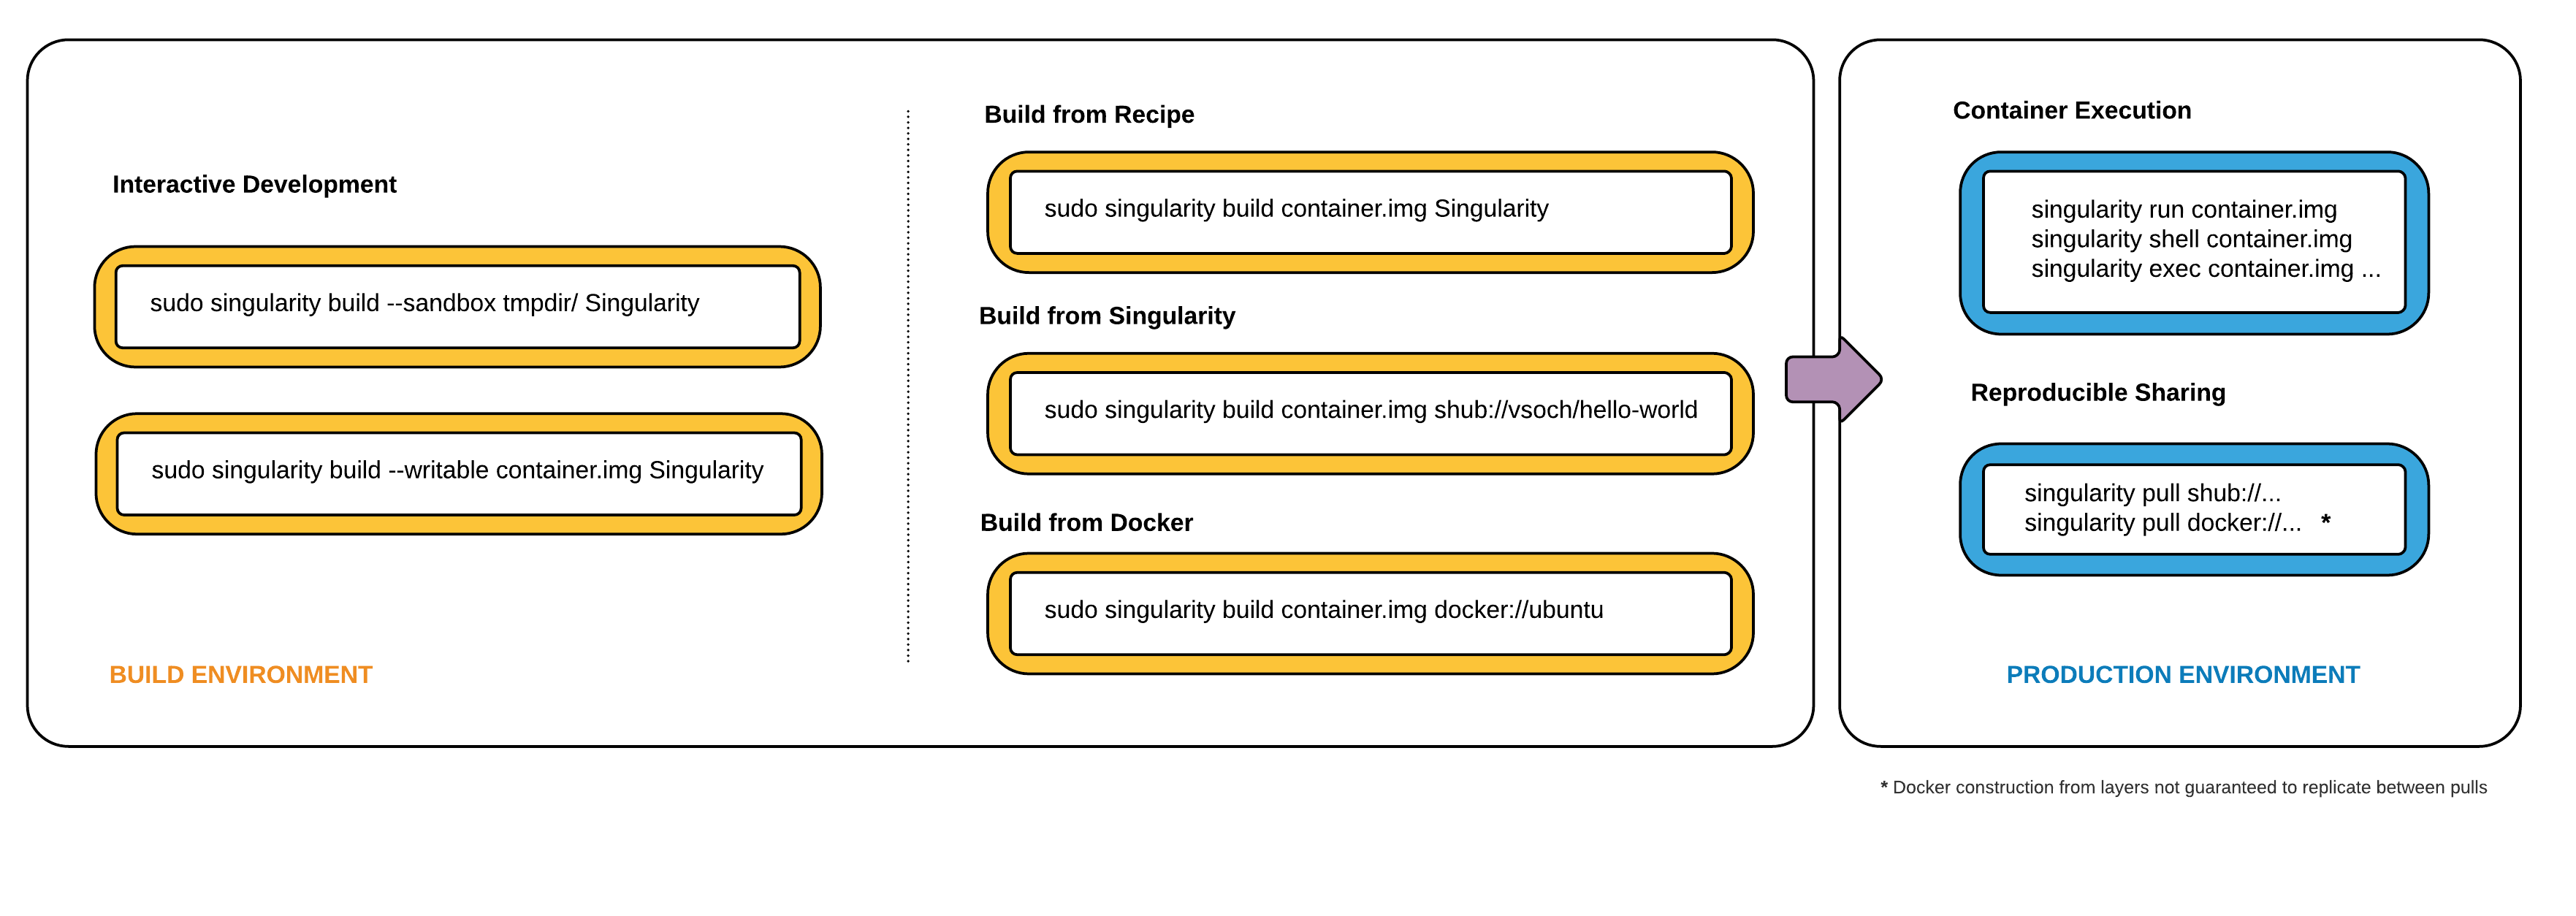
\includegraphics[width=0.5,height=0.5]{flow.png}
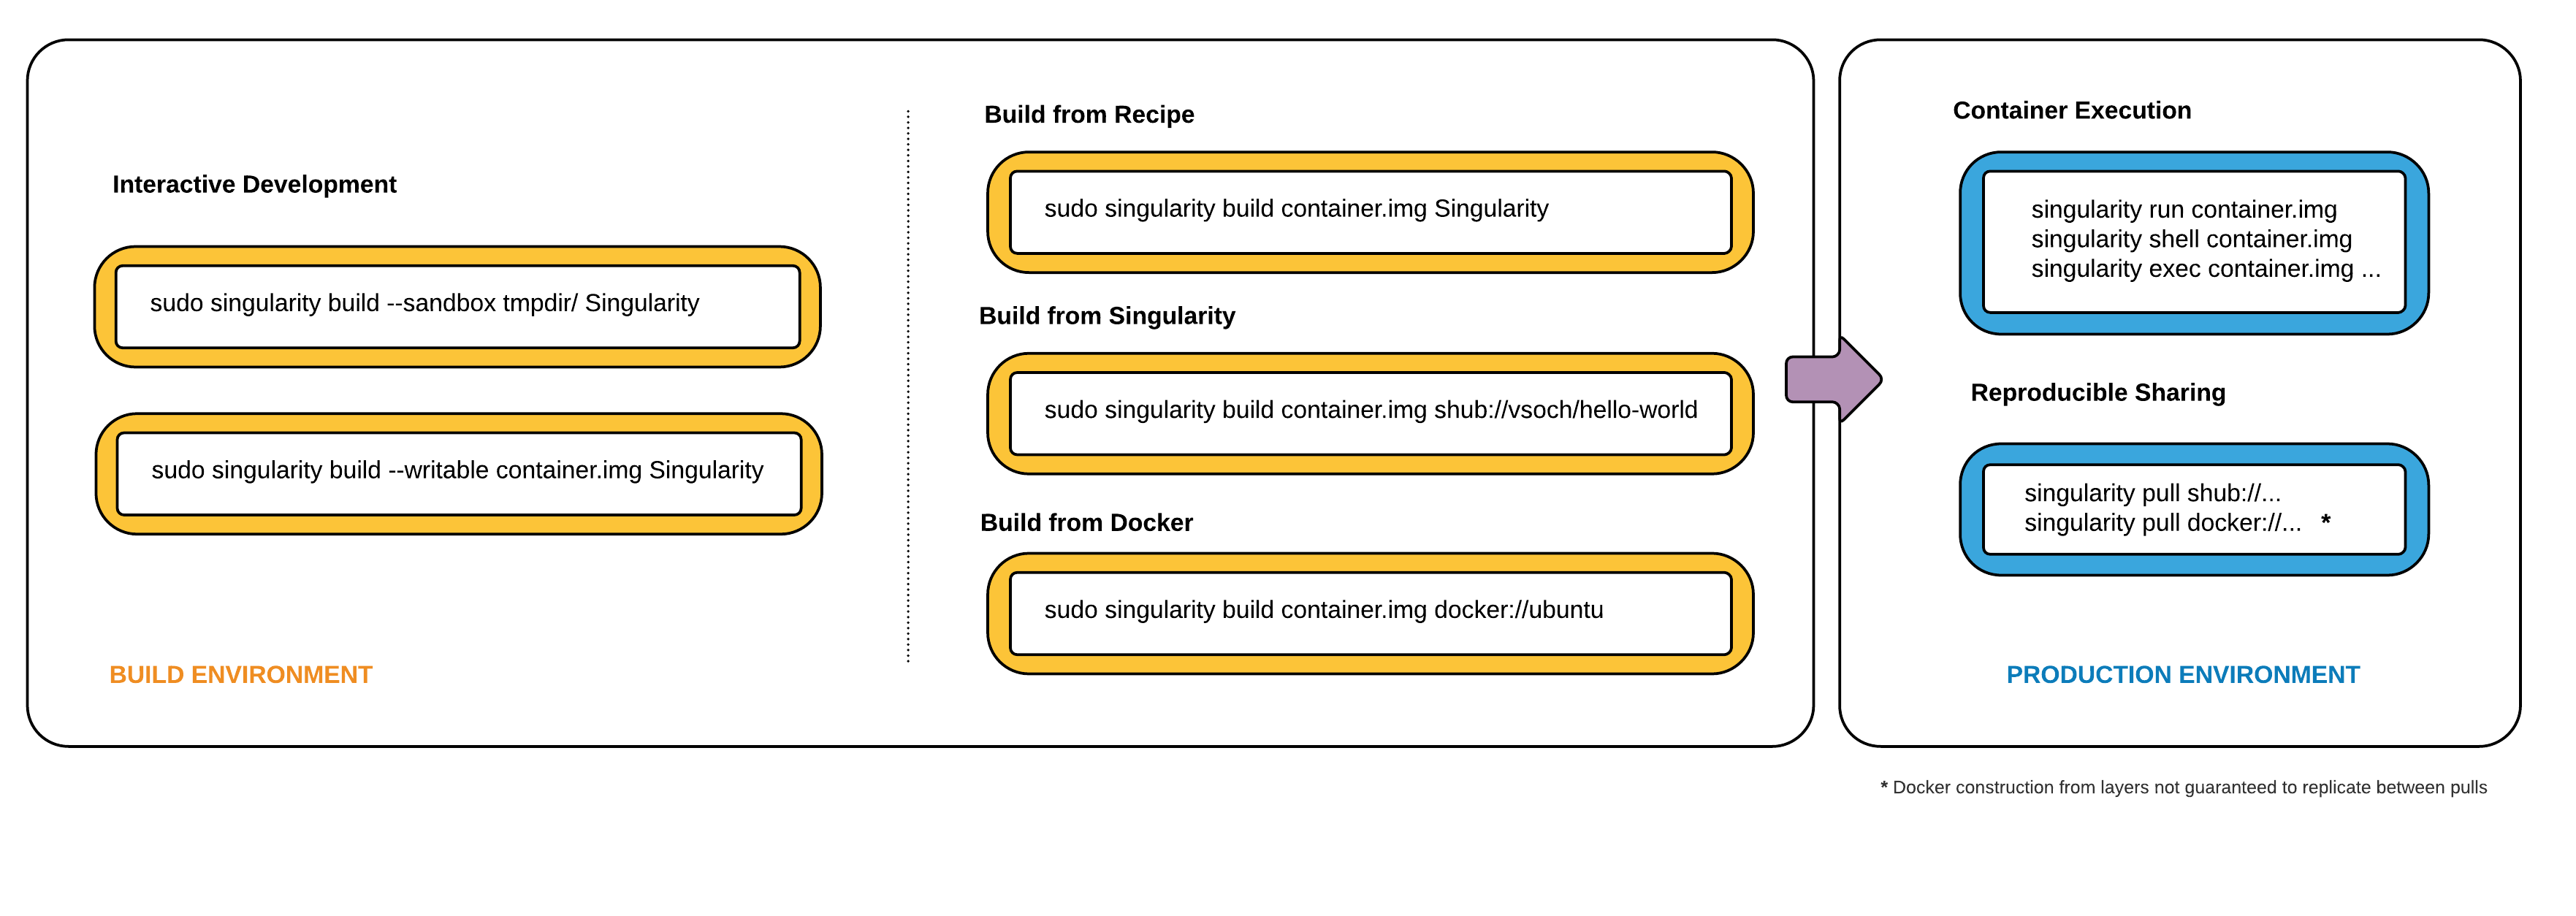
\includegraphics{flow.png}
\caption{Singularity workflow}
\end{figure}

On the left side, you have your build environment: a laptop, workstation, or a server that you control. Here you will (optionally):
\\
\begin{enumerate}
\item develop and test containers using \colorbox{lightgray}{- -sandbox} (build into a writable directory) or  \colorbox{lightgray}{- -writable} (build into a writable ext3 image)
\item build your production containers with a squashfs filesystem.
\end{enumerate}
Once you have the container with the necessary applications, libraries and data inside it can be easily shared to other hosts and executed without requiring root access. A production container should be an immutable object, so if you need to make changes to your container you should go back to your build system with root privileges, rebuild the container with the necessary changes, and then re-upload the container to the production system where you wish to run it.
\subsubsubsection{Singularity Commands}
How do the commands work? Here is where to look for more information:
\\[0.1in]
\begin{itemize}
\item \hyperref[sec:build]{{\textcolor{cyan}{build}}}: Build a container on your user endpoint or build environment
\item \hyperref[sec:exec]{{\textcolor{cyan}{exec}}}: Execute a command to your container
\item \hyperref[sec:inspect]{{\textcolor{cyan}{inspect}}}: See labels, run and test scripts, and environment variables
\item \hyperref[sec:pull]{{\textcolor{cyan}{pull}}}: pull an image from Docker or Singularity Hub
\item \hyperref[sec:run]{{\textcolor{cyan}{run}}}: Run your image as an executable
\item \hyperref[sec:shell]{{\textcolor{cyan}{shell}}}: Shell into your image
\end{itemize}


\noindent\textbf{Image Commands}

\begin{itemize}
\item \hyperref[sec:imageimport]{{\textcolor{cyan}{image.import}}}: import layers or other file content to your image
\item \hyperref[sec:imageexport]{{\textcolor{cyan}{image.export}}}: export the contents of the image to tar or stream
\item \hyperref[sec:imagecreate]{{\textcolor{cyan}{image.create}}}: create a new image, using the old ext3 filesystem
\item \hyperref[sec:imageexpand]{{\textcolor{cyan}{image.expand}}}: increase the size of your image (old ext3)
\end{itemize}

\noindent\textbf{Instance Commands}
\\[0.2in]
\hfill Instances were added in 2.4. This list is brief, and likely to expand with further development.
\begin{itemize}
\item \hyperref[sec:instances]{{\textcolor{cyan}{instances}}}: Start, stop, and list 
container instances
\end{itemize}
\noindent\textbf{Deprecated Commands} The following commands are deprecated in 2.4 and will be removed in future releases.
\begin{itemize}
\item \hyperref[sec:bootstrap]{{\textcolor{cyan}{bootstrap}}}: Bootstrap a container recipe
\end{itemize}
\subsubsection{Support}

Have a question, or need further information? \href{http://singularity.lbl.gov/support}{Reach out to us}.

\subsection{Installation}
\label{sec:installation}

This document will guide you through the process of installing Singularity from source with the version and location of your choice.
\subsubsection{Before you begin}

If you have an earlier version of Singularity installed, you should remove it before executing the installation commands.
\\[0.1in]
These instructions will build Singularity from source on your system. So you will need to have some development tools installed. If you run into missing dependencies, try installing them like so:\\

\subsubsubsection{Ubuntu}

\begin{lstlisting}[frame=single] 
$ sudo apt-get update && \
    sudo apt-get install \
    python \
    dh-autoreconf \
    build-essential \
    libarchive-dev 
\end{lstlisting}

\subsubsubsection{Centos}

\begin{lstlisting}[frame=single] 
$ sudo yum update && \
    sudo yum groupinstall 'Development Tools' && \
    sudo yum install libarchive-devel
\end{lstlisting}


\subsubsection{Install the master branch}

The following commands will install the latest version of the  \href{https://github.com/singularityware/singularity}{GitHub repo} master branch to \colorbox{lightgray}{/usr/local}.

\begin{lstlisting}[frame=single]  
$ git clone https://github.com/singularityware/singularity.git
$ cd singularity
$ ./autogen.sh
$ ./configure --prefix=/usr/local --sysconfdir=/etc
$ make
$ sudo make install
\end{lstlisting}


Note that the installation prefix is \colorbox{lightgray}{/usr/local} but the configuration directory is \colorbox{lightgray}{/etc}. This ensures that the configuration file \colorbox{lightgray}{singularity.conf} is placed in the standard location.\\

If you omit the \colorbox{lightgray}{-{}-sysconfdir} option , the configuration file will be installed in \colorbox{lightgray}{/usr/local/etc}. If you omit the \colorbox{lightgray}{-{}-prefix} option, Singularity will be installed in the \colorbox{lightgray}{/usr/local} directory hierarchy by default. And if you specify a custom directory with the \colorbox{lightgray}{-{}-prefix} option, all of Singularity’s binaries and the configuration file will be installed within that directory. This last option can be useful if you want to install multiple versions of Singularity, install Singularity on a shared system, or if you want to remove Singularity easily after installing it.
\\

\subsubsection{Install a specific release}

The following commands will install a specific release from 
\href{https://github.com/singularityware/singularity/releases}{GitHub releases} page to \colorbox{lightgray}{/usr/local}.\\[0.1in]

\begin{lstlisting}[frame=single]  
$ VER=2.5.1
$ wget https://github.com/singularityware/singularity/releases/download/$VER/singularity-$VER.tar.gz
$ tar xvf singularity-$VER.tar.gz
$ cd singularity-$VER
$ ./configure --prefix=/usr/local --sysconfdir=/etc
$ make
$ sudo make install

\end{lstlisting}

\subsubsection{Install the development branch}

If you want to test a development branch the routine above should be tweaked slightly:\\

\begin{lstlisting}[frame=single]  
$ git clone https://github.com/singularityware/singularity.git
$ cd singularity
$ git fetch
$ git checkout development
$ ./autogen.sh
$ ./configure --prefix=/usr/local --sysconfdir=/etc
$ make
$ sudo make install
\end{lstlisting}

\subsubsection{Remove an old version}

Let’s say that we installed Singularity to \colorbox{lightgray}{/usr/local}. To remove it completely, you need to hit all of the following:


\begin{lstlisting}[frame=single]  
$ sudo rm -rf /usr/local/libexec/singularity
$ sudo rm -rf /usr/local/etc/singularity
$ sudo rm -rf /usr/local/include/singularity
$ sudo rm -rf /usr/local/lib/singularity
$ sudo rm -rf /usr/local/var/lib/singularity/
$ sudo rm /usr/local/bin/singularity
$ sudo rm /usr/local/bin/run-singularity
$ sudo rm /usr/local/etc/bash_completion.d/singularity 
$ sudo rm /usr/local/man/man1/singularity.1
\end{lstlisting}


If you modified the system configuration directory, remove the \colorbox{lightgray}{singularity.conf} file there as well.\\

If you installed Singularity in a custom directory, you need only remove that directory to uninstall Singularity. For instance if you installed singularity with the \colorbox{lightgray}{-{}-prefix=/some/temp/dir} option argument pair, you can remove Singularity like so:

\begin{lstlisting}[frame=single] 
$ sudo rm -rf /some/temp/dir
\end{lstlisting}

What should you do next? You can check out the \hyperref[sec:quickstart]{{\textcolor{cyan}{quickstart}}}  guide, or learn how to interact with your container via the \hyperref[sec:shell]{{\textcolor{cyan}{shell}}}, \hyperref[sec:exec]{{\textcolor{cyan}{exec}}} , or \hyperref[sec:run]{{\textcolor{cyan}{run}}}  commands. Or click \textbf{next} below to continue reading.

\subsection{Build a Container}
\label{sec:buildcontainer}

\colorbox{lightgray}{build} is the “Swiss army knife” of container creation. You can use it to download and assemble existing containers from external resources like \href{https://singularity-hub.org/}{Singularity Hub} and \href{https://hub.docker.com/}{Docker Hub}. You can use it to convert containers between the various formats supported by Singularity. And you can use it in conjunction with a \hyperref[sec:recipefile]{{\textcolor{cyan}{Singularity recipe}}} file to create a container from scratch and customized it to fit your needs.

\subsubsection{Overview}

The \colorbox{lightgray}{build} command accepts a target as input and produces a container as output.\\

The target defines the method that \colorbox{lightgray}{build} uses to create the container. It can be one of the following:\\

\begin{itemize}
\item URI beginning with \textbf{shub://} to build from Singularity Hub
\item URI beginning with \textbf{docker://} to build from Docker Hub
\item path to a \textbf{existing container} on your local machine
\item path to a \textbf{directory} to build from a sandbox
\item path to an \textbf{archive} in .tar or compressed .tar.gz format
\item path to a \textbf{\hyperref[sec:recipefile]{{\textcolor{cyan}{Singularity recipe file}}}}
\end{itemize}

In addition \colorbox{lightgray}{build} can produce containers in three different formats. Formats types can be specified by passing the following options to build.
\\
\begin{itemize}
\item compressed read-only \textbf{squashfs} file system suitable for production (default)
\item writable \textbf{ext3} file system suitable for interactive development ( \colorbox{lightgray}{-{}-writable} option )
\item writable \textbf{(ch)root directory} called a sandbox for interactive development (\colorbox{lightgray}{-{}-sandbox} option)
\end{itemize}

Because \colorbox{lightgray}{build} can accept an existing container as a target and create a container in any of these three formats you can convert existing containers from one format to another.\\

The following diagram illustrates the targets that can be supplied to \colorbox{lightgray}{build} as inputs and the containers \colorbox{lightgray}{build} can produce as outputs. Green arrows represent operations that can be carried out without root privileges (though the container may not perform properly when run as root). Red arrows represent operations that must be carried out with root privileges.


\begin{figure}[h]
\centering
\hspace*{-0.62in}
%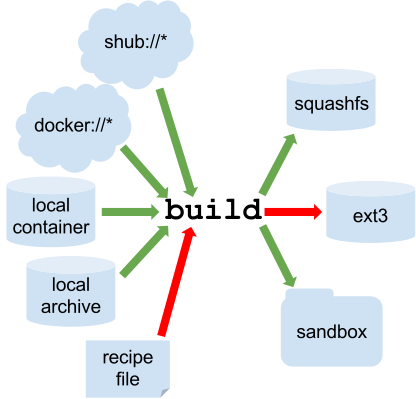
\includegraphics[width=0.5,height=0.5]{build_input_output.png}
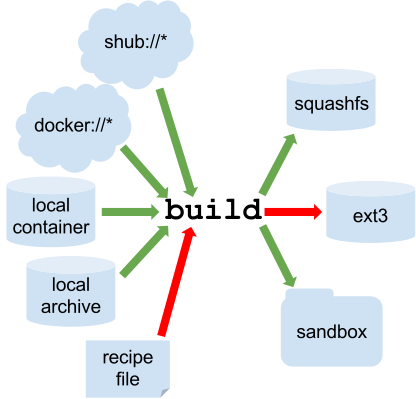
\includegraphics{build_input_output.png}
\caption{Singularity build process}
\end{figure}

\subsubsection{Downloading a existing container from Singularity Hub}
You can use the build command to download a container from Singularity Hub.

\begin{lstlisting}[frame=single]  
$ singularity build lolcow.simg shub://GodloveD/lolcow

\end{lstlisting}

The first argument (\colorbox{lightgray}{lolcow.simg}) specifies a path and name for your container. The second argument \\(\colorbox{lightgray}{shub://GodloveD/lolcow}) gives the Singularity Hub URI from which to download.\\

But default the container will be converted to a compressed, read-only squashfs file. If you want your container in a different format use the \colorbox{lightgray}{-{}-writable} or \colorbox{lightgray}{-{}-sandbox} options.


\subsubsection{Downloading a existing container from Docker Hub}

You can use \colorbox{lightgray}{build} to download layers from Docker Hub and assemble them into Singularity containers.
\begin{lstlisting}[frame=single]  
$ singularity build lolcow.simg docker://godlovedc/lolcow
\end{lstlisting}
\subsubsection{Creating - -writable images and - -sandbox directories}
	\subsubsubsection{- -writable}
	
	If you wanted to create a writable ext3 image similar to those used by Singularity version < 2.4, you could do so with the \colorbox{lightgray}{-{}-writable} option. You must create writable containers as root.
\\[0.1in]
Extending the Singularity Hub example from above:	
\begin{lstlisting}[frame=single]  
$ sudo singularity build --writable lolcow.img shub://GodloveD/lolcow
\end{lstlisting}

	
	The resulting container is writable, but is still mounted as read-only when executed with commands such as \colorbox{lightgray}{run}, \colorbox{lightgray}{exec}, and \colorbox{lightgray}{shell}. To mount the container as read-write when using these commands add the \colorbox{lightgray}{-{}-writable} option to them as well.\\[0.1in]
	To ensure that you have the proper permissions to write to the container as you like, it is also a good idea to make changes as root. For example:
\begin{lstlisting}[frame=single]  
$ sudo singularity shell --writable lolcow.img
\end{lstlisting}	 
	\subsubsubsection{- -sandbox}
	
	If you wanted to create a container within a writable directory (called a sandbox) you could do so with the \colorbox{lightgray}{-{}-sandbox} option. It’s possible to create a sandbox without root privileges, but to ensure proper file permissions it is recommended to do so as root.
	
\begin{lstlisting}[frame=single]  
$ sudo singularity build --sandbox lolcow/ shub://GodloveD/lolcow
\end{lstlisting}	
	
The resulting directory operates just like a container in an image file. You are permitted to make changes and write files within the directory, but those changes will not persist when you are finished using the container. To make your changes persistent, use the \colorbox{lightgray}{-{}-writable} flag when you invoke your container.
\\[0.1in]
Once again, it’s a good idea to do this as root to ensure you have permission to access the files and directories that you want to change.

\begin{lstlisting}[frame=single] 
$ sudo singularity shell --writable lolcow/
\end{lstlisting}
	
\subsubsection{Converting containers from one format to another}

If you already have a container saved locally, you can use it as a target to build a new container. This allows you convert containers from one format to another. For example if you had a squashfs container called \colorbox{lightgray}{production.simg} and wanted to convert it to a writable ext3 container called \colorbox{lightgray}{development.img} you could:


\begin{lstlisting}[frame=single] 
$ sudo singularity build --writable development.img production.simg
\end{lstlisting}

	Similarly, to convert it to a writable directory (a sandbox):\\[0.1in]
	
	
\begin{lstlisting}[frame=single] 
$ singularity build --sandbox development/ production.simg
\end{lstlisting}

If you omit any options you can also convert your sandbox back to a read-only compressed squashfs image suitable for use in a production environment:

\begin{lstlisting}[frame=single] 
$ singularity build production2 development/
\end{lstlisting}

You can convert the three supported container formats using any combination.\\[0.1in]
Use care when converting writable ext3 images or sandbox directories to the default squashfs file format. If changes were made to the writable container before conversion, there is no record of those changes in the Singularity recipe file rendering your container non-reproducible. It is a best practice to build your immutable production containers directly from a Singularity recipe file instead.	
	
\subsubsection{Building containers from Singularity recipe files}

Of course, Singularity recipe files can be used as the target when building a container. For detailed information on writing Singularity recipe files, please see the \hyperref[sec:recipefile]{{\textcolor{cyan}{Container Recipes docs}}}.\\
Let’s say you already have the following container recipe file called \colorbox{lightgray}{Singularity}, and you want to use it to build a container.

\begin{lstlisting}[frame=single] 
Bootstrap: docker
From: ubuntu:16.04

%post
    apt-get -y update
    apt-get -y install fortune cowsay lolcat

%environment
    export LC_ALL=C
    export PATH=/usr/games:$PATH

%runscript
    fortune | cowsay | lolcat
\end{lstlisting}

You can do so with the following command.	

\begin{lstlisting}[frame=single] 
$ sudo singularity build lolcow.simg Singularity 
\end{lstlisting}

The command requires \colorbox{lightgray}{sudo} just as installing software on your local machine requires root privileges.

	\subsubsubsection{- -force}
	You can build into the same container multiple times (though the results may be unpredictable and it is generally better to delete your container and start from scratch).\\[0.1in]
By default if you build into an existing container, the \colorbox{lightgray}{build} command will skip the steps involved in adding a new base. You can override this default with the \colorbox{lightgray}{-{}-force} option requiring that a new base OS is bootstrapped into the existing container. This behavior does not delete the existing OS, it just adds the new OS on top of the existing one.\\[0.1in]
Use care with this option: you may get results that you did not expect.

	\subsubsubsection{- -section}
	
	If you only want to build a single section of your Singularity recipe file use the  \colorbox{lightgray}{-{}-section} option. For instance, if you have edited the \colorbox{lightgray}{\%environment} section of a long Singularity recipe and don’t want to completely re-build the container, you could re-build only the \ \colorbox{lightgray}{\%environment} section like so:
	
\begin{lstlisting}[frame=single] 
$ sudo singularity build --section environment image.simg Singularity
\end{lstlisting}	
	
Under normal build conditions, the Singularity recipe file is saved into a container’s meta-data so that there is a record showing how the container was built. Using the \colorbox{lightgray}{-{}-section} option may render this meta-data useless, so use care if you value reproducibility.

	\subsubsubsection{- -notest}
	
If you don’t want to run the \colorbox{lightgray}{\%test} section during the container build, you can skip it with the \colorbox{lightgray}{-{}-notest} option. For instance, maybe you are building a container intended to run in a production environment with GPUs. But perhaps your local build resource does not have GPUs. You want to include a \colorbox{lightgray}{\%test} section that runs a short validation but you don’t want your build to exit with an error because it cannot find a GPU on your system.

\begin{lstlisting}[frame=single]
$ sudo singularity build GPU.simg --notest Singularity
\end{lstlisting}

	\subsubsubsection{- -checks}
	
	Checks are a new feature (in 2.4) that offer an easy way for an admin to define a security (or any other kind of check) to be run on demand for a Singularity image. They are defined (and run) via different tags.\\[0.1in]

\begin{lstlisting}[frame=single]
CHECKS OPTIONS:
    -c|--checks    enable checks
    -t|--tag       specify a check tag (not default)
    -l|--low       Specify low threshold (all checks, default) 
    -m|--med       Perform medium and high checks
    -h|--high      Perform only checks at level high
\end{lstlisting}	
    
    When you add the \colorbox{lightgray}{-{}-checks} option along with applicable tags to the \colorbox{lightgray}{build} command Singularity will run the desired checks on your container at build time. See \colorbox{lightgray}{singularity check --help} for available tags.
	
\subsubsection{More Build topics}

\begin{itemize}
\item If you want to \textbf{customize the cache location} (where Docker layers are downloaded on your system), specify Docker credentials, or any custom tweaks to your build environment, see \hyperref[sec:buildenv]{{\textcolor{cyan}{build environment}}}.
\item If you want to make internally \textbf{modular containers}, check out the getting started guide \href{https://sci-f.github.io/tutorials}{here}
\item If you want to \textbf{build your containers} on Singularity Hub, (because you don’t have root access on a Linux machine or want to host your container on the cloud) check out \href{https://github.com/singularityhub/singularityhub.github.io/wiki}{this guide}
\end{itemize}


\subsection{Build Environment}
\label{sec:buildenv}

It’s commonly the case that you want to customize your build environment, such as specifying a custom cache directory for layers, or sending your Docker Credentials to the registry endpoint. Here we will discuss those things

\subsubsection{Cache Folders}

To make download of layers for build and \hyperref[sec:pull]{{\textcolor{cyan}{pull}}} faster and less redundant, we use a caching strategy. By default, the Singularity software will create a set of folders in your  \colorbox{lightgray}{\$HOME} directory for docker layers, Singularity Hub images, and Docker metadata, respectively:

\begin{lstlisting}[frame=single] 
$HOME/.singularity
$HOME/.singularity/docker
$HOME/.singularity/shub
$HOME/.singularity/metadata 
\end{lstlisting}

Fear not, you have control to customize this behavior! If you don’t want the cache to be created (and a temporary directory will be used), set \colorbox{lightgray}{SINGULARITY\_DISABLE\_CACHE} to True/yes, or if you want to move it elsewhere, set \colorbox{lightgray}{SINGULARITY\_CACHEDIR} to the full path where you want to cache. Remember that when you run commands as sudo this will use root’s home at \colorbox{lightgray}{/root} and not your user’s home.
\subsubsection{Temporary Folders}
\label{sec:temporaryfolders}
Singularity also uses some temporary directories to build the squashfs filesystem, so this temp space needs to be large enough to hold the entire resulting Singularity image. By default this happens in \colorbox{lightgray}{/tmp} but can be overridden by setting \colorbox{lightgray}{SINGULARITY\_TMPDIR} to the full path where you want the squashfs temp files to be stored. Since images are typically built as root, be sure to set this variable in root’s environment.
\\[0.1in]
If you are building an image on the fly, for example

\begin{lstlisting}[frame=single]
singularity exec docker://busybox /bin/sh 
\end{lstlisting}

by default a temporary runtime directory is created that looks like \colorbox{lightgray}{/tmp/.singularity-runtime.xxxxxxxx}. This can be problematic for some \colorbox{lightgray}{/tmp} directories that are hosted at Jetstream/OpenStack, Azure, and possibly EC2, which are very small. If you need to change the location of this runtime, then \textbf{export} the variable\\ \colorbox{lightgray}{\$SINGULARITY\_LOCALCACHEDIR}.

\begin{lstlisting}[frame=single]
SINGULARITY_LOCALCACHEDIR=/tmp/pancakes
export SINGULARITY_LOCALCACHEDIR
singularity exec docker://busybox /bin/sh
\end{lstlisting}

The above runtime folder would be created under\\[0.1in]
\colorbox{lightgray}{/tmp/pancakes/.singularity-runtime.xxxxxxxx}

\subsubsection{Pull Folder}

For details about customizing the output location of 
\hyperref[sec:pull]{{\textcolor{cyan}{pull}}}, see the 
\hyperref[sec:pull]{{\textcolor{cyan}{pull docs}}}. You have the similar ability to set it to be something different, or to customize the name of the pulled image.


\subsubsection{Environment Variables}

All environmental variables are parsed by Singularity python helper functions, and specifically the file \href{https://github.com/singularityware/singularity/blob/master/libexec/python/defaults.py}{defaults.py} is a gateway between variables defined at runtime, and pre-defined defaults. By way of import from the file, variables set at runtime do not change if re-imported. This was done intentionally to prevent changes during the execution, and could be changed if needed. For all variables, the order of operations works as follows:\\
\begin{enumerate}
\item First preference goes to environment variable set at runtime
\item Second preference goes to default defined in this file
\item Then, if neither is found, null is returned except in the case that \colorbox{lightgray}{required=True}. A \colorbox{lightgray}{required=True} variable not found will system exit with an error.
\item Variables that should not be displayed in debug logger are set with \colorbox{lightgray}{silent=True}, and are only reported to be defined.
\end{enumerate}

For boolean variables, the following are acceptable for True, with any kind of capitalization or not:

\begin{lstlisting}[frame=single]
("yes", "true", "t", "1","y")
\end{lstlisting}

\subsubsection{Cache}

The location and usage of the cache is also determined by environment variables.\\[0.1in]
\textbf{SINGULARITY\_DISABLE\_CACHE} If you want to disable the cache, this means is that the layers are written to a temporary directory. Thus, if you want to disable cache and write to a temporary folder, simply set  \colorbox{lightgray}{SINGULARITY\_DISABLE\_CACHE} to any true/yes value. By default, the cache is not disabled.\\[0.1in]

\textbf{SINGULARITY\_CACHEDIR} Is the base folder for caching layers and singularity hub images. If not defined, it uses default of  \colorbox{lightgray}{\$HOME/.singularity}. If defined, the defined location is used instead. \\If  \colorbox{lightgray}{SINGULARITY\_DISABLE\_CACHE} is set to True, this value is ignored in favor of a temporary directory. For specific sub-types of things to cache, subdirectories are created (by python), including  \colorbox{lightgray}{\$SINGULARITY\_CACHEDIR/docker} for docker layers and  \colorbox{lightgray}{\$SINGULARITY\_CACHEDIR/shub} for Singularity Hub images. If the cache is not created, the Python script creates it.\\[0.1in]

\textbf{SINGULARITY\_PULLFOLDER} While this isn’t relevant for build, since build is close to pull, we will include it here. By default, images are pulled to the present working directory. The user can change this variable to change that.\\[0.1in]

\textbf{SINGULARITY\_TMPDIR} Is the base folder for squashfs image temporary building. If not defined, it uses default of  \colorbox{lightgray}{\$TEMPDIR}. If defined, the defined location is used instead.\\[0.1in]

\textbf{SINGULARITY\_LOCALCACHEDIR} Is the temporary folder (default  \colorbox{lightgray}{/tmp}) to generate runtime folders (containers “on the fly”) typically a  \colorbox{lightgray}{run},  \colorbox{lightgray}{exec}, or  \colorbox{lightgray}{shell} or a  \colorbox{lightgray}{docker://} image. This is different from where downloaded layers are cached ( \colorbox{lightgray}{\$SINGULARITY\_CACHEDIR}) or pulled ( \colorbox{lightgray}{\$SINGULARITY\_PULLFOLDER}) or where a (non on-the-fly build) happens ( \colorbox{lightgray}{\$SINGULARITY\_TMPDIR}). See \hyperref[sec:temporaryfolders]{{\textcolor{cyan}{temporary folders}}} above for an example. You can generally determine the value of this setting by running a command with  \colorbox{lightgray}{-{}-debug}, and seeing the last line “Removing directory:”\\[0.1in]

\begin{lstlisting}[frame=single]
singularity --debug run docker://busybox echo "pizza!"
...
DEBUG   [U=1000,P=960]     s_rmdir()                                 Removing directory: /tmp/.singularity-runtime.oArO0k
\end{lstlisting}

	\subsubsubsection{Defaults}
	
	The following variables have defaults that can be customized by you via environment variables at runtime.

	\paragraph{Docker}\tab{}\\[0.2in]\textbf{DOCKER\_API\_BASE} Set as \colorbox{lightgray}{index.docker.io}, which is the name of the registry. In the first version of Singularity we parsed the Registry argument from the build spec file, however now this is removed because it can be obtained directly from the image name (eg, \colorbox{lightgray}{registry/namespace/repo:tag}). If you don’t specify a registry name for your image, this default is used. If you have trouble with your registry being detected from the image URI, use this variable.\\[0.1in]

\textbf{DOCKER\_API\_VERSION} Is the version of the Docker Registry API currently being used, by default now is \colorbox{lightgray}{v2}.\\[0.1in]

\textbf{DOCKER\_OS} This is exposed via the exported environment variable \colorbox{lightgray}{SINGULARITY\_DOCKER\_OS} and pertains to images that reveal a version 2 manifest with a \href{https://docs.docker.com/registry/spec/manifest-v2-2/#manifest-list}{manifest list}. In the case that the list is present, we must choose an operating system (this variable) and an architecture (below). The default is \colorbox{lightgray}{linux}.\\[0.1in]

\textbf{DOCKER\_ARCHITECTURE} This is exposed via the exported environment variable \\
\colorbox{lightgray}{SINGULARITY\_DOCKER\_ARCHITECTURE} and the same applies as for the \colorbox{lightgray}{DOCKER\_OS} with regards to being used in context of a list of manifests. In the case that the list is present, we must choose an architecture (this variable) and an os (above). The default is \colorbox{lightgray}{amd64}, and other common ones include \colorbox{lightgray}{arm}, \colorbox{lightgray}{arm64}, \colorbox{lightgray}{ppc64le}, \colorbox{lightgray}{386}, and \colorbox{lightgray}{s390x}.\\[0.1in]

\textbf{NAMESPACE} Is the default namespace, \colorbox{lightgray}{library}.

\textbf{RUNSCRIPT\_COMMAND} Is not obtained from the environment, but is a hard coded default ("/bin/bash"). This is the fallback command used in the case that the docker image does not have a CMD or ENTRYPOINT.\\[0.1in]

\textbf{TAG} Is the default tag, \colorbox{lightgray}{latest}.\\[0.1in]

\textbf{SINGULARITY\_NOHTTPS} This is relevant if you want to use a registry that doesn’t have https, and it speaks for itself. If you export the variable \colorbox{lightgray}{SINGULARITY\_NOHTTPS} you can force the software to not use https when interacting with a Docker registry. This use case is typically for use of a local registry.

\paragraph{Singularity Hub}

\textbf{SHUB\_API\_BASE} The default base for the Singularity Hub API, which is\\ \colorbox{lightgray}{https://singularity-hub.org/api}. If you deploy your own registry, you don’t need to change this, you can again specify the registry name in the \colorbox{lightgray}{shub://} URI.

	\subsubsubsection{General}

\textbf{SINGULARITY\_PYTHREADS} The Python modules use threads (workers) to download layer files for Docker, and change permissions. By default, we will use 9 workers, unless the environment variable \colorbox{lightgray}{SINGULARITY\_PYTHREADS} is defined.\\[0.1in]

\textbf{SINGULARITY\_COMMAND\_ASIS} By default, we want to make sure the container running process gets passed forward as the current process, so we want to prefix whatever the Docker command or entrypoint is with \colorbox{lightgray}{exec}. We also want to make sure that following arguments get passed, so we append \colorbox{lightgray}{"\$@"}. Thus, some entrypoint or cmd might look like this:

\begin{lstlisting}[frame=single]  
/usr/bin/python
\end{lstlisting}

and we would parse it into the runscript as:

\begin{lstlisting}[frame=single]  
exec /usr/bin/python "$@"
\end{lstlisting}

However, it might be the case that the user does not want this. For this reason, we have the environmental variable \colorbox{lightgray}{RUNSCRIPT\_COMMAND\_ASIS}. If defined as yes/y/1/True/true, etc., then the runscript will remain as \colorbox{lightgray}{/usr/bin/python}.

\subsection{Container Recipes}
\label{sec:recipefile}

A Singularity Recipe is the driver of a custom build, and the starting point for designing any custom container. It includes specifics about installation software, environment variables, files to add, and container metadata. You can even write a help section, or define modular components in the container called based on the \href{https://sci-f.github.io/}{Scientific Filesystem}.

\subsubsection{Overview}

A Singularity Recipe file is divided into several parts:
\begin{enumerate}
\item \textbf{Header}: The Header describes the core operating system to build within the container. Here you will configure the base operating system features that you need within your container. Examples of this include, what distribution of Linux, what version, what packages must be part of a core install.
\item \textbf{Sections}: The rest of the definition is comprised of sections, sometimes called scriptlets or blobs of data. Each section is defined by a \colorbox{lightgray}{\%} character followed by the name of the particular section. All sections are optional. Sections that are executed at build time are executed with the \colorbox{lightgray}{/bin/sh} interpreter and can accept \colorbox{lightgray}{/bin/sh} options. Similarly, sections that produce scripts to be executed at runtime can accept options intended for \colorbox{lightgray}{/bin/sh}
\end{enumerate}

Please see the \href{https://github.com/singularityware/singularity/tree/master/examples}{examples} directory in the \href{https://github.com/singularityware/singularity}{Singularity source code} for some ideas on how to get started.\\[0.1in]

	\subsubsubsection{Header}
	
	The header is at the top of the file, and tells Singularity the base Operating System that it should use to build the container. It is composed of several keywords. Specifically:
	
	\begin{itemize}
	\item \colorbox{lightgray}{Bootstrap}: references the kind of base you want to use (e.g., docker, debootstrap, shub). For example, a shub bootstrap will pull containers for shub as bases. A Docker bootstrap will pull docker layers to start your image. For a full list see \hyperref[sec:buildcontainer]{{\textcolor{cyan}{build}}} 
	\item \colorbox{lightgray}{From}: is the named container (shub) or reference to layers (Docker) that you want to use (e.g., vsoch/hello-world)
	\end{itemize}
	
Depending on the value assigned to \colorbox{lightgray}{Bootstrap:}, other keywords may also be valid in the header.
\\[0.1in]
For example, a very minimal Singularity Hub build might look like this:

\begin{lstlisting}[frame=single] 
Bootstrap: shub
From: vsoch/hello-world 
\end{lstlisting}

A build that uses a mirror to install Centos-7 might look like this:
	

\begin{lstlisting}[frame=single] 
Bootstrap: yum
OSVersion: 7
MirrorURL: http://mirror.centos.org/centos-%{OSVERSION}/%{OSVERSION}/os/$basearch/
Include: yum
\end{lstlisting}
	
	
	Each build base requires particular details during build time. You can read about them and see examples at the following links:\\[0.1in]
	
	\begin{itemize}
	\item  \href{http://singularity.lbl.gov/build-shub}{shub} (images hosted on Singularity Hub)
	\item  \href{http://singularity.lbl.gov/build-docker-module}{docker} (images hosted on Docker Hub)
	\item  \href{http://singularity.lbl.gov/build-localimage}{localimage} (images saved on your machine)
	\item  \href{http://singularity.lbl.gov/build-yum}{yum} (yum based systems such as CentOS and Scientific Linux)
	\item  \href{http://singularity.lbl.gov/build-debootstrap}{debootstrap} (apt based systems such as Debian and Ubuntu)
	\item  \href{http://singularity.lbl.gov/build-arch}{arch} (Arch Linux)
	\item  \href{http://singularity.lbl.gov/build-busybox}{busybox} (BusyBox)
	\item  \href{http://singularity.lbl.gov/build-zypper}{zypper} (zypper based systems such as Suse and OpenSuse)
	\end{itemize}
	
	
	\subsubsubsection{Sections}
	
	The main content of the bootstrap file is broken into sections. Different sections add different content or execute commands at different times during the build process. Note that if any command fails, the build process will halt.\\[0.1in]
Let’s add each section to our container to see how it works. For each section, we will build the container from the recipe (a file called Singularity) as follows:

\begin{lstlisting}[frame=single] 
$ sudo singularity build roar.simg Singularity
\end{lstlisting}


\paragraph{\%help}
\label{sec:writehelpdocs}
You don’t need to do much programming to add a \colorbox{lightgray}{\%help} section to your container. Just write it into a section:\\[0.1in]

\begin{lstlisting}[frame=single] 
Bootstrap: docker
From: ubuntu

%help
Help me. I'm in the container.
\end{lstlisting}

And it will work when the user asks the container for help.

\begin{lstlisting}[frame=single] 
$ singularity help roar.simg 

Help me. I'm in the container.
\end{lstlisting}
	
\paragraph{\%setup}

Commands in the \%setup section are executed on the host system outside of the container after the base OS has been installed. For versions earlier than 2.3 if you need files during \%post, you should copy files from your host to \$SINGULARITY\_ROOTFS to move them into the container. For \textgreater 2.3 you can add files to the container (added before \%post) using the \%files section. We can see the difference between \%setup and \%post in the following asciicast:
\\[0.2in]
In the above, we see that copying something to \colorbox{lightgray}{\$SINGULARITY\_ROOTFS} during \colorbox{lightgray}{\%setup} was successful to move the file into the container, but copying during \colorbox{lightgray}{\%post} was not. Let’s add a setup to our current container, just writing a file to the root of the image:

\begin{lstlisting}[frame=single]  
Bootstrap: docker
From: ubuntu

%help
Help me. I'm in the container.

%setup
    touch ${SINGULARITY_ROOTFS}/tacos.txt
    touch avocados.txt
\end{lstlisting}

Importantly, notice that the avocados file isn’t relative to \$SINGULARITY\_ROOTFS, so we would expect it not to be in the image. Is tacos there?

\begin{lstlisting}[frame=single]  
$ singularity exec roar.simg ls /
bin   environment  lib	  mnt	root  scif	   sys	      usr
boot  etc	   lib64  opt	run   singularity  **tacos.txt**  var
dev   home	   media  proc	sbin  srv	   tmp
\end{lstlisting}

Yes! And avocados.txt isn’t inside the image, but in our present working directory:

\begin{lstlisting}[frame=single]  
$ ls
avocados.txt   roar.simg   Singularity
\end{lstlisting}

\paragraph{\%files}
		
If you want to copy files from your host system into the container, you should do so using the  \colorbox{lightgray}{\%files} section. Each line is a pair of  \colorbox{lightgray}{\textless source\textgreater}  and  \colorbox{lightgray}{\textless destination \textgreater}, where the source is a path on your host system, and the destination is a path in the container.\\[0.1in]

The \colorbox{lightgray}{\%files} section uses the traditional  \colorbox{lightgray}{cp} command, so the \href{https://linux.die.net/man/1/cp}{same conventions apply}\\[0.1in]

Files are copied \textbf{before} any \colorbox{lightgray}{\%post} or installation procedures for Singularity versions \textgreater 2.3. If you are using a legacy version, files are copied after \colorbox{lightgray}{\%post} so you must do this via \colorbox{lightgray}{\%setup}. Let’s add the avocado.txt into the container, to join tacos.txt.\\[0.1in]

\begin{lstlisting}[frame=single] 
Bootstrap: docker
From: ubuntu

%help
Help me. I'm in the container.

# Both of the below are copied before %post
# 1. This is how to copy files for legacy < 2.3
%setup
    touch ${SINGULARITY_ROOTFS}/tacos.txt
    touch avocados.txt

# 2. This is how to copy files for >= 2.3
%files
    avocados.txt
    avocados.txt /opt 
\end{lstlisting}

Notice that I’m adding the same file to two different places. For the first, I’m adding the single file to the root of the image. For the second, I’m adding it to opt. Does it work?

\begin{lstlisting}[frame=single] 
$ singularity exec roar.simg ls /
 singularity exec roar.simg ls /
**avocados.txt**  dev	   home   media  proc  sbin	    srv        tmp
bin	      environment  lib	  mnt	 root  scif	    sys        usr
boot	      etc	   lib64  opt	 run   singularity  **tacos.txt**  var

$ singularity exec roar.simg ls /opt
**avocados.txt**
 
\end{lstlisting}

We have avocados!

\paragraph{\%labels}

To store metadata with your container, you can add them to the \colorbox{lightgray}{\%labels} section. They will be stored in the file \colorbox{lightgray}{/.singularity.d/labels.json} as metadata within your container. The general format is a \colorbox{lightgray}{LABELNAME} followed by a \colorbox{lightgray}{LABELVALUE}. Labels from Docker bootstraps will be carried forward here. Let’s add to our example:

\begin{lstlisting}[frame=single]  
Bootstrap: docker
From: ubuntu

%help
Help me. I'm in the container.

%setup
    touch ${SINGULARITY_ROOTFS}/tacos.txt
    touch avocados.txt

%files
    avocados.txt
    avocados.txt /opt    

%labels
    Maintainer Vanessasaurus
    Version v1.0
\end{lstlisting}

The easiest way to see labels is to inspect the image:

\begin{lstlisting}[frame=single]  
$ singularity inspect roar.simg
{
    "org.label-schema.usage.singularity.deffile.bootstrap": "docker",
    "MAINTAINER": "Vanessasaurus",
    "org.label-schema.usage.singularity.deffile": "Singularity",
    "org.label-schema.usage": "/.singularity.d/runscript.help",
    "org.label-schema.schema-version": "1.0",
    "VERSION": "v1.0",
    "org.label-schema.usage.singularity.deffile.from": "ubuntu",
    "org.label-schema.build-date": "2017-10-02T17:00:23-07:00",
    "org.label-schema.usage.singularity.runscript.help": "/.singularity.d/runscript.help",
    "org.label-schema.usage.singularity.version": "2.3.9-development.g3dafa39",
    "org.label-schema.build-size": "1760MB"
}
\end{lstlisting}

You’ll notice some other labels that are captured automatically from the build process. You can read more about labels and metadata  \hyperref[sec:envandmetadata]{{\textcolor{cyan}{here}}} .

\paragraph{\%environment}
		
	As of Singularity 2.3, you can add environment variables to your Singularity Recipe in a section called \colorbox{lightgray}{\%environment}. Keep in mind that these environment variables are sourced at runtime and not at build time. This means that if you need the same variables during build time, you should also define them in your \colorbox{lightgray}{\%post} section. Specifically:\\[0.1in]

 \begin{itemize}
 \item \textbf{during build}: the \colorbox{lightgray}{\%environment} section is written to a file in the container’s metadata folder. This file is not sourced.
 \item \textbf{during runtime}: the file written to the container’s metadata folder is sourced.
 \end{itemize}
Since the file is ultimately sourced, you should generally use the same conventions that you might use in a bashrc or profile. In the example below, the variables \colorbox{lightgray}{VADER} \colorbox{lightgray}{LUKE} and \colorbox{lightgray}{SOLO} would not be available during build, but when the container is finished and run:

\begin{lstlisting}[frame=single]  
Bootstrap: docker
From: ubuntu

%help
Help me. I'm in the container.

%setup
    touch ${SINGULARITY_ROOTFS}/tacos.txt
    touch avocados.txt

%files
    avocados.txt
    avocados.txt /opt    

%labels
    Maintainer Vanessasaurus
    Version v1.0

%environment
    VADER=badguy
    LUKE=goodguy
    SOLO=someguy
    export VADER LUKE SOLO
\end{lstlisting}

For the rationale behind this approach and why we do not source the \%environment section at build time, refer to this issue. When the container is finished, you can easily see environment variables also with inspect, and this is done by showing the file produced above:

\begin{lstlisting}[frame=single]  
$ singularity inspect -e roar.simg # Custom environment shell code should follow

    VADER=badguy
    LUKE=goodguy
    SOLO=someguy
    export VADER LUKE SOLO
\end{lstlisting}
    
or in the case of variables generated at build time, you can add environment variables to your container in the \colorbox{lightgray}{\%post} section (see below) using the following syntax: 

\begin{lstlisting}[frame=single] 
%post
    echo 'export JAWA_SEZ=wutini' >> $SINGULARITY_ENVIRONMENT 
\end{lstlisting}

    When we rebuild, is it added to the environment?
    
\begin{lstlisting}[frame=single] 
singularity exec roar.simg env | grep JAWA
JAWA_SEZ=wutini
\end{lstlisting}

Where are all these environment variables going? Inside the container is a metadata folder located at \colorbox{lightgray}{/.singularity.d}, and a subdirectory \colorbox{lightgray}{env} for environment scripts that are sourced. Text in the \colorbox{lightgray}{\%environment} section is appended to a file called \colorbox{lightgray}{/.singularity.d/env/90-environment.sh}. Text redirected to the \colorbox{lightgray}{\$SINGULARITY\_ENVIRONMENT} variable will added to a file called \colorbox{lightgray}{/.singularity.d/env/91-environment.sh}. At runtime, scripts in \colorbox{lightgray}{/.singularity/env} are sourced in order. This means that variables in \colorbox{lightgray}{\$SINGULARITY\_ENVIRONMENT} take precedence over those added via \colorbox{lightgray}{\%environment}. Note that you won’t see these variables in the inspect output, as inspect only shows the contents added from \colorbox{lightgray}{\%environment}.\\[0.1in]

See \hyperref[sec:envandmetadata]{{\textcolor{cyan}{Environment and Metadata}}} for more information about the \colorbox{lightgray}{\%labels} and \colorbox{lightgray}{\%environment} sections.


		\paragraph{\%post}
		
		Commands in the \colorbox{lightgray}{\%post} section are executed within the container after the base OS has been installed at build time. This is where the meat of your setup will live, including making directories, and installing software and libraries. We will jump from our simple use case to show a more realistic scientific container. Here we are installing yum, openMPI, and other dependencies for a Centos7 bootstrap:
		
\begin{lstlisting}[frame=single]  
%post
    echo "Installing Development Tools YUM group"
    yum -y groupinstall "Development Tools"
    echo "Installing OpenMPI into container..."

    # Here we are at the base, /, of the container
    git clone https://github.com/open-mpi/ompi.git

    # Now at /ompi
    cd ompi
    ./autogen.pl
    ./configure --prefix=/usr/local
    make
    make install

    /usr/local/bin/mpicc examples/ring_c.c -o /usr/bin/mpi_ring
\end{lstlisting}		
		
		You cannot copy files from the host to your container in this section, but you can of course download with commands like \colorbox{lightgray}{git clone} and \colorbox{lightgray}{wget} and \colorbox{lightgray}{curl}.


		\paragraph{\%runscript}
		\label{sec:runscript}
		
The \colorbox{lightgray}{\%runscript} is another scriptlet, but it does not get executed during bootstrapping. Instead it gets persisted within the container to a file (or symlink for later versions) called \colorbox{lightgray}{/singularity} which is the execution driver when the container image is run (either via the \colorbox{lightgray}{singularity run} command or via executing the container directly).\\[0.1in]

When the  \colorbox{lightgray}{\%runscript} is executed, all options are passed along to the executing script at runtime, this means that you can (and should) manage argument processing from within your runscript. Here is an example of how to do that, adding to our work in progress:

\begin{lstlisting}[frame=single]  
Bootstrap: docker
From: ubuntu

%help
Help me. I'm in the container.

%setup
    touch ${SINGULARITY_ROOTFS}/tacos.txt
    touch avocados.txt

%files
    avocados.txt
    avocados.txt /opt    

%labels
    Maintainer Vanessasaurus
    Version v1.0

%environment
    VADER=badguy
    LUKE=goodguy
    SOLO=someguy
    export VADER LUKE SOLO


%post
    echo 'export JAWA_SEZ=wutini' >> $SINGULARITY_ENVIRONMENT

%runscript
    echo "Rooooar!"
    echo "Arguments received: $*"
    exec echo "$@"
\end{lstlisting}
  
  In this particular runscript, the arguments are printed as a single string (\colorbox{lightgray}{\$*}) and then they are passed to echo via a quoted array (\colorbox{lightgray}{"\$@"}) which ensures that all of the arguments are properly parsed by the executed command. Using the \colorbox{lightgray}{exec} command is like handing off the calling process to the one in the container. The final command (the echo) replaces the current entry in the process table (which originally was the call to Singularity). This makes it so the runscript shell process ceases to exist, and the only process running inside this container is the called echo command. This could easily be another program like python, or an analysis script. Running it, it works as expected:
  
\begin{lstlisting}[frame=single] 
$ singularity run roar.simg 
Rooooar!
Arguments received: 

$ singularity run roar.simg one two
Rooooar!
Arguments received: one two
one two
\end{lstlisting}
		
\paragraph{\%test}
You may choose to add a\colorbox{lightgray}{ \%test} section to your definition file. This section will be run at the very end of the build process and will give you a chance to validate the container during the bootstrap process. You can also execute this scriptlet through the container itself, such that you can always test the validity of the container itself as you transport it to different hosts. Extending on the above Open MPI \colorbox{lightgray}{\%post}, consider this real world example:

\begin{lstlisting}[frame=single] 
%test
    /usr/local/bin/mpirun --allow-run-as-root /usr/bin/mpi_test
\end{lstlisting}


This is a simple Open MPI test to ensure that the MPI is build properly and communicates between processes as it should.\\[0.1in]

If you want to build without running tests (for example, if the test needs to be done in a different environment), you can do so with the \colorbox{lightgray}{ --notest} argument:\\[0.1in]


\begin{lstlisting}[frame=single] 
$ sudo singularity build --notest mpirun.simg Singularity
\end{lstlisting}

This argument is useful in cases where you need hardware that is available during runtime, but is not available on the host that is building the image.

\subsubsection{Apps}

What if you want to build a single container with two or three different apps that each have their own runscripts and custom environments? In some circumstances, it may be redundant to build different containers for each app with almost equivalent dependencies.\\[0.1in]

Starting in Singularity 2.4 all of the above commands can also be used in the context of internal modules called \hyperref[sec:scifapps]{{\textcolor{cyan}{apps}}}  based on the \href{https://sci-f.github.io/}{Standard Container Integration Format}. For details on apps, see the \hyperref[sec:scifapps]{{\textcolor{cyan}{apps}}} documentation. For a quick rundown of adding an app to your container, here is an example runscript:

\begin{lstlisting}[frame=single] 
Bootstrap: docker
From: ubuntu

%environment
    VADER=badguy
    LUKE=goodguy
    SOLO=someguy
    export VADER LUKE SOLO

%labels
   Maintainer Vanessasaur

##############################
# foo
##############################

%apprun foo
    exec echo "RUNNING FOO"

%applabels foo
   BESTAPP=FOO
   export BESTAPP

%appinstall foo
   touch foo.exec

%appenv foo
    SOFTWARE=foo
    export SOFTWARE

%apphelp foo
    This is the help for foo.

%appfiles foo
   avocados.txt


##############################
# bar
##############################

%apphelp bar
    This is the help for bar.

%applabels bar
   BESTAPP=BAR
   export BESTAPP

%appinstall bar
    touch bar.exec

%appenv bar
    SOFTWARE=bar
    export SOFTWARE
\end{lstlisting}

Importantly, note that the apps can exist alongside any and all of the primary sections (e.g. \colorbox{lightgray}{\%post} or \colorbox{lightgray}{\%runscript}), and the new \colorbox{lightgray}{\%appinstall} section is the equivalent of \%post but for an app. The title sections (\colorbox{lightgray}{\#\#\#\#\#\#}) aren’t necessary or required, they are just comments to show you the different apps. The ordering isn’t important either, you can have any mixture of sections anywhere in the file after the header. The primary difference is now the container can perform any of it’s primary functions in the context of an app:\\[0.1in]

\textbf{What apps are installed in the container?}

\begin{lstlisting}[frame=single]  
$ singularity apps roar.simg 
bar
foo
\end{lstlisting}

\textbf{Help me with bar!}

\begin{lstlisting}[frame=single]  
$ singularity help --app bar roar.simg
This is the help for bar.
\end{lstlisting}

\textbf{Run foo}
\begin{lstlisting}[frame=single]  
singularity run --app foo roar.simg 
RUNNING FOO
\end{lstlisting}


\textbf{Show me the custom environments}\\[0.1in]

Remember how we defined the same environment variable, SOFTWARE for each of foo and bar? We can execute a command to search the list of active environment variables with grep to see if the variable changes depending on the app we specify:

\begin{lstlisting}[frame=single]  
$ singularity exec --app foo roar.simg env | grep SOFTWARE
SOFTWARE=foo
$ singularity exec --app bar roar.simg env | grep SOFTWARE
SOFTWARE=bar
\end{lstlisting}

\subsubsection{Examples}

For more examples, for real world scientific recipes we recommend you look at other containers on  \href{https://singularity-hub.org/}{Singularity Hub}. For examples of different bases, look at the examples folder for the most up-to-date examples. For apps, including snippets and tutorial with more walk throughs, see \href{https://sci-f.github.io/}{SCI-F Apps Home}.\\[0.1in]

\subsubsection{Best Practices for Build Recipes}

When crafting your recipe, it is best to consider the following:

\begin{enumerate}
\item 
To make your container internally modular, use \hyperref[sec:scifapps]{{\textcolor{cyan}{SCI-F apps}}}. Shared dependencies (between app modules) can go under \colorbox{lightgray}{\%post}.
\item
For global installs to \colorbox{lightgray}{\%post}, install packages, programs, data, and files into operating system locations (e.g. not \colorbox{lightgray}{/home}, \colorbox{lightgray}{/tmp}, or any other directories that might get commonly binded on).
\item Make your container speak for itself. If your runscript doesn’t spit out help, write a \colorbox{lightgray}{\%help} or\colorbox{lightgray}{\%post} or \colorbox{lightgray}{\%apphelp} section. A good container tells the user how to interact with it.
\item If you require any special environment variables to be defined, add them the \colorbox{lightgray}{\%environment} and \colorbox{lightgray}{\%appenv} sections of the build recipe.
\item Files should never be owned by actual users, they should always be owned by a system account (UID less than 500).
\item Ensure that the container’s \colorbox{lightgray}{/etc/passwd}, \colorbox{lightgray}{/etc/group}, \colorbox{lightgray}{/etc/shadow}, and no other sensitive files have anything but the bare essentials within them.
\item It is encouraged to build containers from a recipe instead of a sandbox that has been manually changed. This ensures greatest possibility of reproducibility and mitigates the black box effect.
\end{enumerate}

Are you a recipe pro and now ready to build? Take a look at the  \hyperref[sec:buildcontainer]{{\textcolor{cyan}{build}}} documentation.

\subsection{Singularity Flow}

This document describes a suggested “best-practices” workflow for building, running, and managing your containers.\\[0.1in]
There are generally two ways to get images. You either want to pull an image file as is, or (more likely) build your own custom image. We will start with talking about build, and the many different use cases it affords.


\label{sec:singularityflow}
\subsubsection{Building Images}

If you read the \hyperref[sec:quickstart]{{\textcolor{cyan}{quick start}}}, you probably remember that building images from a Docker base does not require a \hyperref[sec:recipefile]{{\textcolor{cyan}{Singularity recipe}}}. However, if you do want to build and customize your image, you can create a \hyperref[sec:recipefile]{{\textcolor{cyan}{Singularity recipe}}} text file, which is a simple text file that describes how the container should be made.\\[0.1in]

	\subsubsubsection{The Singularity Flow}

	The diagram below is a visual depiction of how you can use Singularity to build images. The high level idea is that we have two environments:
	
	\begin{itemize}
	\item a \textbf{build} environment (where you have sudo privileges) to test and build your container
	\item a \textbf{production} environment where you run your container
\end{itemize}

\begin{figure}[h]
\centering
%{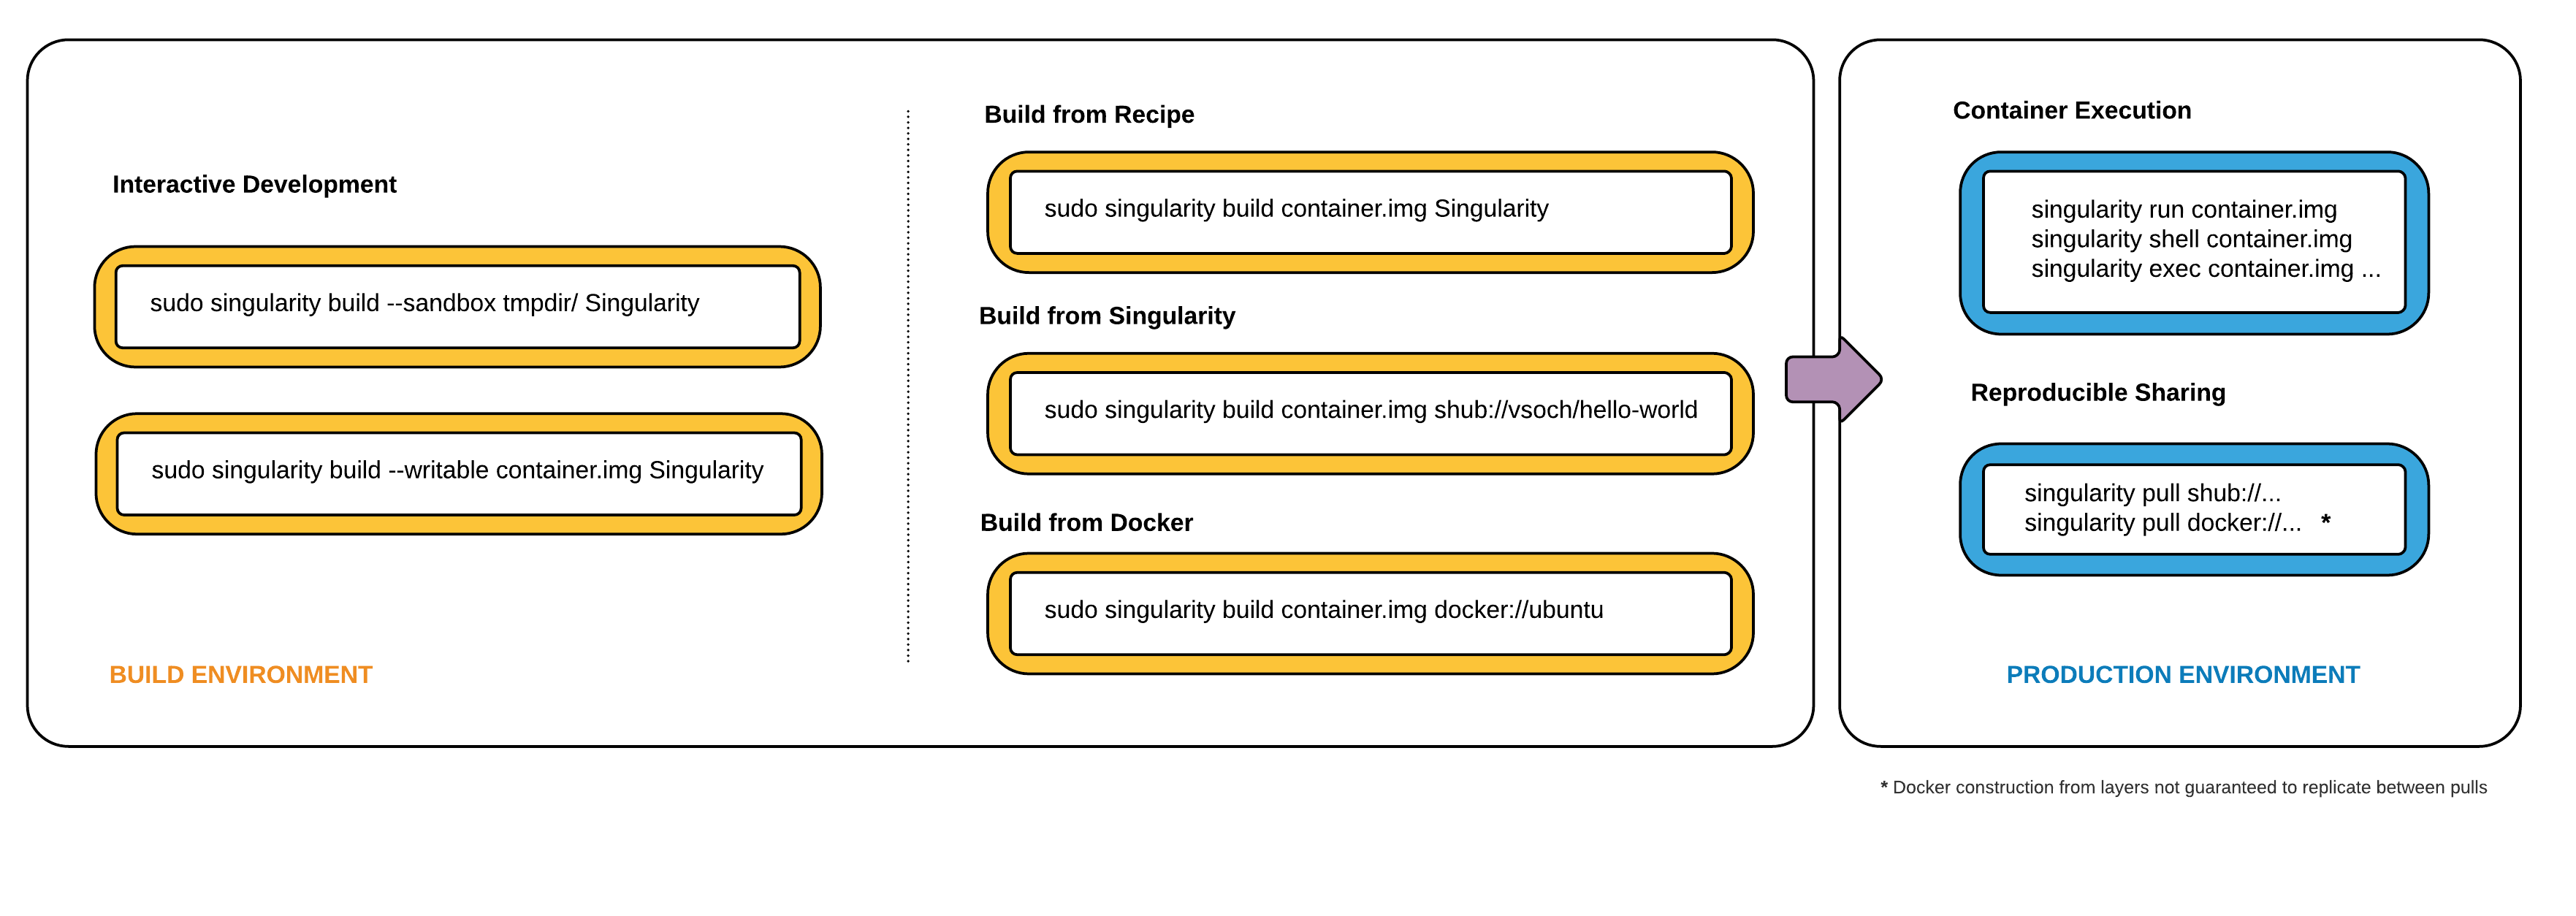
\includegraphics[width=0.5,height=0.5]{flow.png}}
{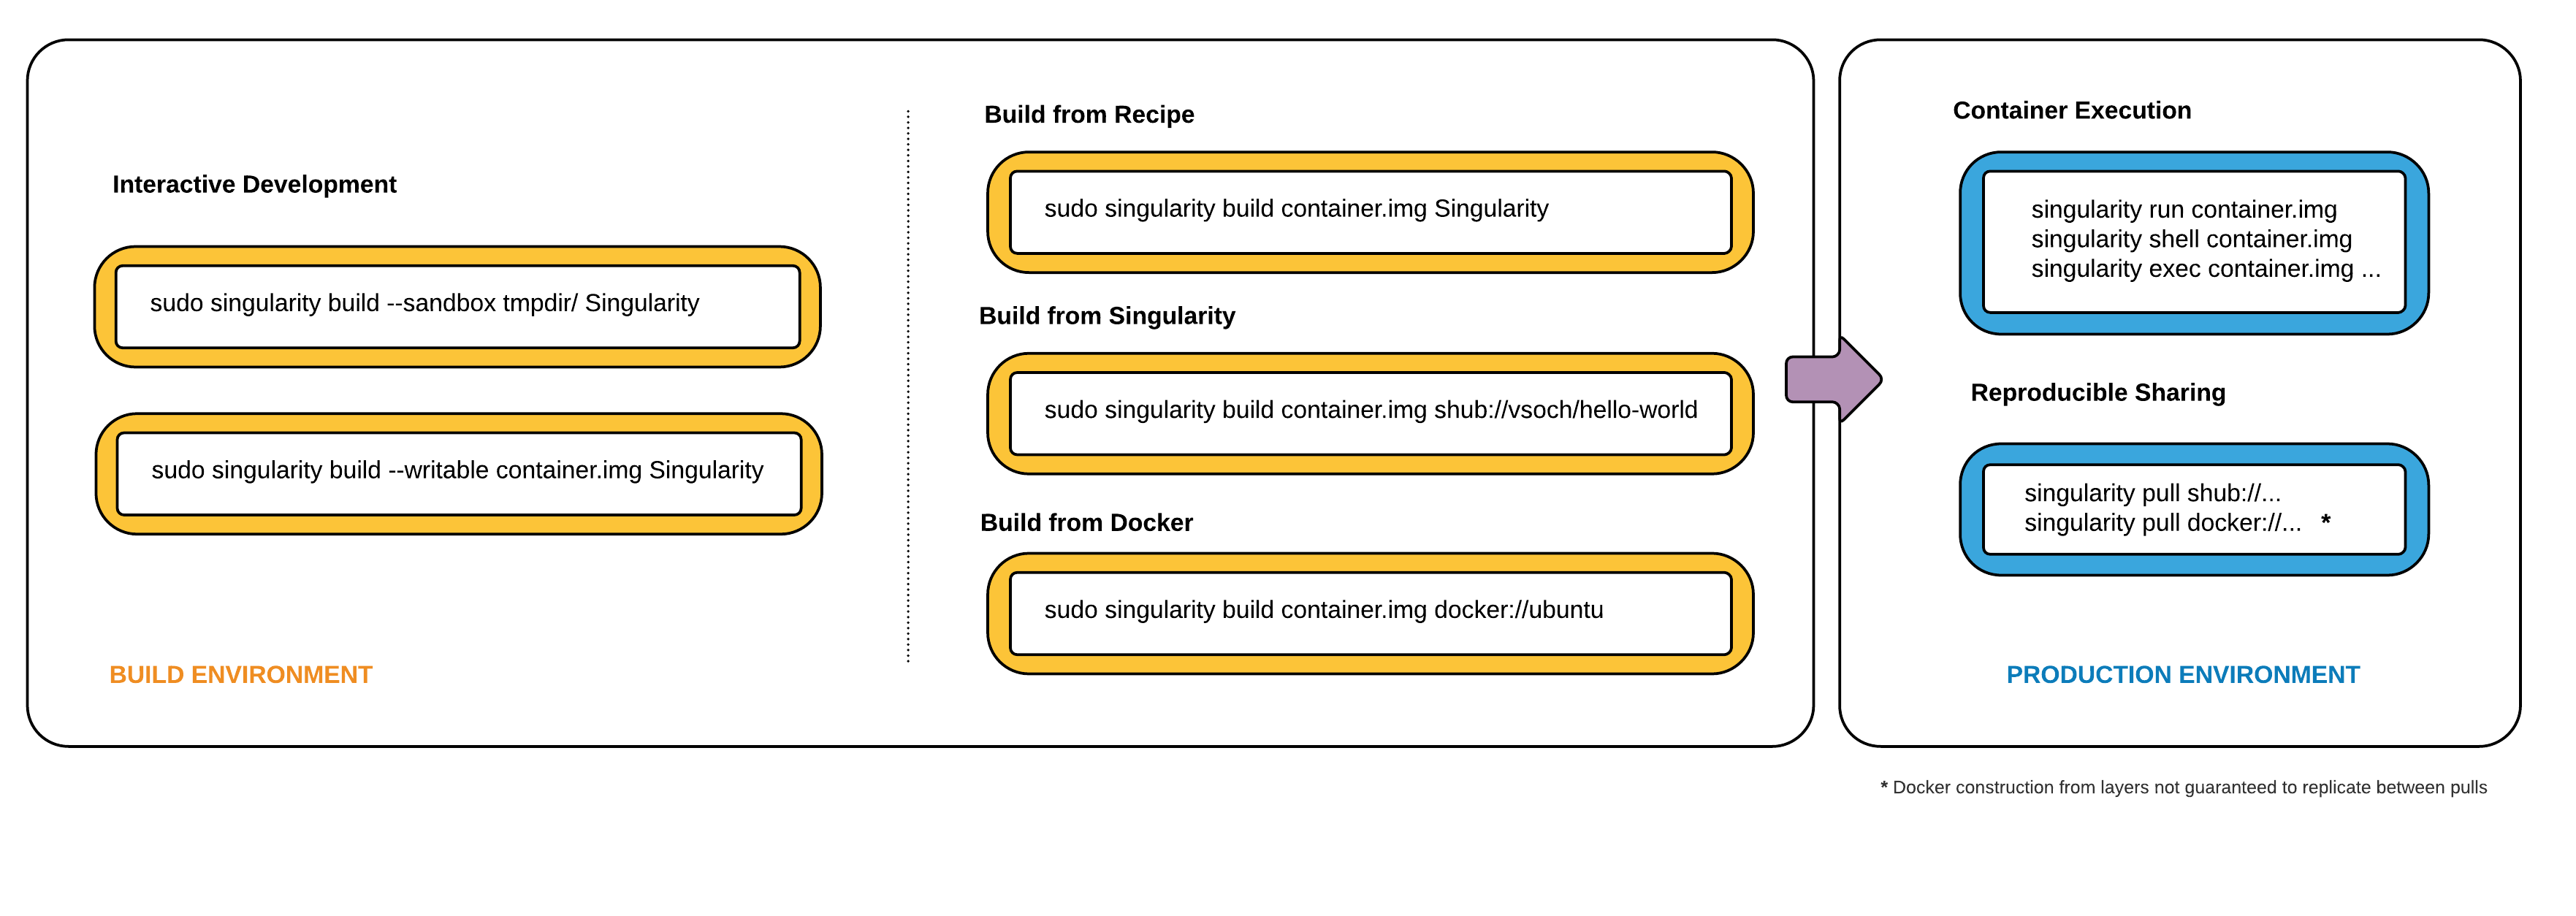
\includegraphics{flow.png}}
\caption{Singularity workflow}
\end{figure}

Singularity production images are immutable. This is a feature added as of Singularity 2.4, and it ensures a higher level of reproducibility and verification of images. To read more about the details, check out the \hyperref[sec:buildcontainer]{{\textcolor{cyan}{build}}} docs. However, immutability is not so great when you are testing, debugging, or otherwise want to quickly change your image. We will proceed by describing a typical workflow of developing first, building a final image, and using it in production.

\subsubsubsection{Development Commands}
	If you want a writable image or folder for developing, you have two options:
\begin{itemize}
\item build into a directory that has writable permissions using the \colorbox{lightgray}{-{}-sandbox} option
\item build into an ext3 image file, that has writable permissions with the \colorbox{lightgray}{-{}-writable} option
\end{itemize}


In both cases you will need to execute your container with the \colorbox{lightgray}{-{}-writable} option at runtime for your changes to be persistent.

		\paragraph{Sandbox Folder}
		
		To build into a folder (we call this a “sandbox”) just ask for it:\\
	
\begin{lstlisting}[frame=single]  
$ sudo singularity build --sandbox ubuntu/ docker://ubuntu
Docker image path: index.docker.io/library/ubuntu:latest
Cache folder set to /root/.singularity/docker
Importing: base Singularity environment
Importing: /root/.singularity/docker/sha256:9fb6c798fa41e509b58bccc5c29654c3ff4648b608f5daa67c1aab6a7d02c118.tar.gz
Importing: /root/.singularity/docker/sha256:3b61febd4aefe982e0cb9c696d415137384d1a01052b50a85aae46439e15e49a.tar.gz
Importing: /root/.singularity/docker/sha256:9d99b9777eb02b8943c0e72d7a7baec5c782f8fd976825c9d3fb48b3101aacc2.tar.gz
Importing: /root/.singularity/docker/sha256:d010c8cf75d7eb5d2504d5ffa0d19696e8d745a457dd8d28ec6dd41d3763617e.tar.gz
Importing: /root/.singularity/docker/sha256:7fac07fb303e0589b9c23e6f49d5dc1ff9d6f3c8c88cabe768b430bdb47f03a9.tar.gz
Importing: /root/.singularity/metadata/sha256:22e289880847a9a2f32c62c237d2f7e3f4eae7259bf1d5c7ec7ffa19c1a483c8.tar.gz
Building image from sandbox: ubuntu/
Singularity container built: ubuntu/
\end{lstlisting}

We now have a folder with the entire ubuntu OS, plus some Singularity metadata, plopped in our present working directory.\\[0.1in]

\begin{lstlisting}[frame=single] 
 $ tree -L 1 ubuntu
ubuntu
├── bin
├── boot
├── dev
├── environment -> .singularity.d/env/90-environment.sh
├── etc
├── home
├── lib
├── lib64
├── media
├── mnt
├── opt
├── proc
├── root
├── run
├── sbin
├── singularity -> .singularity.d/runscript
├── srv
├── sys
├── tmp
├── usr
└── var
\end{lstlisting}

And you can shell into it just like a normal container.

\begin{lstlisting}[frame=single]  
$ singularity shell ubuntu
Singularity: Invoking an interactive shell within container...

Singularity ubuntu:~/Desktop> touch /hello.txt
touch: cannot touch '/hello.txt': Permission denied
\end{lstlisting}

		You can make changes to the container (assuming you have the proper permissions to do so) but those changes will disappear as soon as you exit. To make your changes persistent across sessions, use the \colorbox{lightgray}{-{}-writable} option. It’s also a good practice to shell into your container as root to ensure you have permissions to write where you like.\\
		
\begin{lstlisting}[frame=single]  
$ sudo singularity shell ubuntu
Singularity: Invoking an interactive shell within container...

Singularity ubuntu:/home/vanessa/Desktop> touch /hello.txt

\end{lstlisting}		
	
		\paragraph{Writable Image}
		
		If you prefer to work with a writable image file rather than a directory, you can perform a similar development build and specify the \colorbox{lightgray}{-{}-writable} option. This will produce an image that is writable with an ext3 file system. Unlike the sandbox, it is a single image file.

\begin{lstlisting}[frame=single]  

$ sudo singularity build --writable ubuntu.img docker://ubuntu
Docker image path: index.docker.io/library/ubuntu:latest
Cache folder set to /root/.singularity/docker
Importing: base Singularity environment
Importing: /root/.singularity/docker/sha256:9fb6c798fa41e509b58bccc5c29654c3ff4648b608f5daa67c1aab6a7d02c118.tar.gz
Importing: /root/.singularity/docker/sha256:3b61febd4aefe982e0cb9c696d415137384d1a01052b50a85aae46439e15e49a.tar.gz
Importing: /root/.singularity/docker/sha256:9d99b9777eb02b8943c0e72d7a7baec5c782f8fd976825c9d3fb48b3101aacc2.tar.gz
Importing: /root/.singularity/docker/sha256:d010c8cf75d7eb5d2504d5ffa0d19696e8d745a457dd8d28ec6dd41d3763617e.tar.gz
Importing: /root/.singularity/docker/sha256:7fac07fb303e0589b9c23e6f49d5dc1ff9d6f3c8c88cabe768b430bdb47f03a9.tar.gz
Importing: /root/.singularity/metadata/sha256:22e289880847a9a2f32c62c237d2f7e3f4eae7259bf1d5c7ec7ffa19c1a483c8.tar.gz
Building image from sandbox: /tmp/.singularity-build.VCHPpP
Creating empty Singularity writable container 130MB
Creating empty 162MiB image file: ubuntu.img
Formatting image with ext3 file system
Image is done: ubuntu.img
Building Singularity image...
Cleaning up...
Singularity container built: ubuntu.img

\end{lstlisting}

You can use this image with commands like \colorbox{lightgray}{shell}, \colorbox{lightgray}{exec}, \colorbox{lightgray}{run}, and if you want to change the image you must use the \colorbox{lightgray}{-{}-writable} flag. As before, it’s a good idea to issue these commands as root to ensure you have the proper permissions to write.

\begin{lstlisting}[frame=single]
$ sudo singularity shell --writable ubuntu.img  
\end{lstlisting}
	
\begin{quote}
Development Tip! When building containers, it often is the case that you will have a lot of testing of installation commands, and if building a production image, one error will stop the entire build. If you interactively write the build recipe with one of these writable containers, you can debug as you go, and then build the production (squashfs) container without worrying that it will error and need to be started again.
\end{quote}		
		
	\subsubsubsection{Production Commands}
	
	Let’s set the scene - we just finished building our perfect hello world container. It does a fantastic hello-world analysis, and we have written a paper on it! We now want to build an immutable container - meaning that if someone obtained our container and tried to change it, they could not. They could easily use the same recipe that you used (it is provided as metadata inside the container), or convert your container to one of the writable formats above using \colorbox{lightgray}{build}. So your work can still be extended.

		\paragraph{Recommended Production Build}
		
		What we want for production is a build into a  \href{https://en.wikipedia.org/wiki/SquashFS}{squashfs image} . Squashfs is a read only, and compressed filesystem, and well suited for confident archive and re-use of your hello-world. To build a production image, just remove the extra options:
		
\begin{lstlisting}[frame=single] 
sudo singularity build ubuntu.simg docker://ubuntu
Docker image path: index.docker.io/library/ubuntu:latest
Cache folder set to /root/.singularity/docker
Importing: base Singularity environment
Importing: /root/.singularity/docker/sha256:9fb6c798fa41e509b58bccc5c29654c3ff4648b608f5daa67c1aab6a7d02c118.tar.gz
Importing: /root/.singularity/docker/sha256:3b61febd4aefe982e0cb9c696d415137384d1a01052b50a85aae46439e15e49a.tar.gz
Importing: /root/.singularity/docker/sha256:9d99b9777eb02b8943c0e72d7a7baec5c782f8fd976825c9d3fb48b3101aacc2.tar.gz
Importing: /root/.singularity/docker/sha256:d010c8cf75d7eb5d2504d5ffa0d19696e8d745a457dd8d28ec6dd41d3763617e.tar.gz
Importing: /root/.singularity/docker/sha256:7fac07fb303e0589b9c23e6f49d5dc1ff9d6f3c8c88cabe768b430bdb47f03a9.tar.gz
Importing: /root/.singularity/metadata/sha256:22e289880847a9a2f32c62c237d2f7e3f4eae7259bf1d5c7ec7ffa19c1a483c8.tar.gz
Building Singularity image...
Cleaning up...
Singularity container built: ubuntu.simg 
\end{lstlisting}
		\paragraph{Production Build from Sandbox}
		
		We understand that it might be wanted to build a Singularity (squashfs) from a previous development image. While we advocate for the first approach, we support this use case. To do this, given our folder called “ubuntu/” we made above:
		
\begin{lstlisting}[frame=single]
sudo singularity build ubuntu.simg ubuntu/  
\end{lstlisting}		

It could be the case that a cluster maintains a “working” base of container folders (with writable) and then builds and provides production containers to its users.\\[0.1in]

If you want to go through this entire process without having singularity installed locally, or without leaving your cluster, you can build images using \href{https://github.com/singularityhub/singularityhub.github.io/wiki}{singularity hub}.
		
\subsection{Bind Paths and Mounts}
\label{sec:bindpaths}

If \href{http://singularity.lbl.gov/docs-config#user-bind-control-boolean-defaultyes}{enabled by the system administrator}, Singularity allows you to map directories on your host system to directories within your container using bind mounts. This allows you to read and write data on the host system with ease.

\subsubsection{Overview}

When Singularity ‘swaps’ the host operating system for the one inside your container, the host file systems becomes inaccessible. But you may want to read and write files on the host system from within the container. To enable this functionality, Singularity will bind directories back in via two primary methods: system-defined bind points and conditional user-defined bind points.

	\subsubsubsection{System-defined bind points}
	
	The system administrator has the ability to define what bind points will be included automatically inside each container. The bind paths are locations on the host’s root file system which should also be visible within the container. Some of the bind paths are automatically derived (e.g. a user’s home directory) and some are statically defined (e.g. bind path in the Singularity configuration file). In the default configuration, the directories \colorbox{lightgray}{\$HOME}, \colorbox{lightgray}{/tmp}, \colorbox{lightgray}{/proc}, \colorbox{lightgray}{/sys}, and \colorbox{lightgray}{/dev} are among the system-defined bind points.


	\subsubsubsection{User-defined bind points}
	
	If the system administrator has \href{http://singularity.lbl.gov/docs-config#user-bind-control-boolean-defaultyes}{enabled user control of binds}, you will be able to request your own bind points within your container.
	\\[0.1in]
	To \textit{mount} a bind path inside the container, a \textbf{bind point} must be defined within the container. The bind point is a directory within the container that Singularity can use to bind a directory on the host system. This means that if you want to bind to a point within the container such as \colorbox{lightgray}{/global}, that directory must already exist within the container.	\\[0.1in]
	It is, however, possible that the system administrator has enabled a Singularity feature called \href{http://singularity.lbl.gov/docs-config#enable-overlay-boolean-defaultno}{overlay in the Singularity configuration file}. This will cause the bind points to be created on an as-needed basis in an overlay file system so that the underlying container is not modified. But because the overlay feature is not always enabled or is unavailable in the kernels of some older host systems, it may be necessary for container standards to exist to ensure portability from host to host.\\[0.1in]

\paragraph{Specifying Bind Paths}
		
Many of the Singularity commands such as \colorbox{lightgray}{run}, \colorbox{lightgray}{exec}, and \colorbox{lightgray}{shell} take the \colorbox{lightgray}{-{}-bind}/\colorbox{lightgray}{-B} command-line option to specify bind paths, in addition to the \colorbox{lightgray}{SINGULARITY\_BINDPATH} environment variable. This option’s argument is a comma-delimited string of bind path specifications in the format \colorbox{lightgray}{src[:dest[:opts]]}, where \colorbox{lightgray}{src} and \colorbox{lightgray}{dest} are outside and inside paths. If \colorbox{lightgray}{dest} is not given, it is set equal to \colorbox{lightgray}{src}. Mount options (\colorbox{lightgray}{opts}) may be specified as \colorbox{lightgray}{ro} (read-only) or \colorbox{lightgray}{rw} (read/write, which is the default). The \colorbox{lightgray}{-{}-bind/-B} option can be specified multiple times, or a comma-delimited string of bind path specifications can be used.\\[0.1in]

Here’s an example of using the \colorbox{lightgray}{-B} option and binding \colorbox{lightgray}{/tmp} on the host to \colorbox{lightgray}{/scratch} in the container (\colorbox{lightgray}{/scratch} does not need to already exist in the container if file system overlay is enabled):	

\begin{lstlisting}[frame=single]  
$ singularity shell -B /tmp:/scratch /tmp/Centos7-ompi.img
Singularity: Invoking an interactive shell within container...

Singularity.Centos7-ompi.img> ls /scratch
ssh-7vywtVeOez  systemd-private-cd84c81dda754fe4a7a593647d5a5765-ntpd.service-12nMO4
\end{lstlisting}


You can bind multiple directories in a single command with this syntax:\\

\begin{lstlisting}[frame=single]
$ singularity shell -B /opt,/data:/mnt /tmp/Centos7-ompi.img
\end{lstlisting}


This will bind \colorbox{lightgray}{/opt} on the host to \colorbox{lightgray}{/opt} in the container and \colorbox{lightgray}{/data} on the host to \colorbox{lightgray}{/mnt} in the container. Using the environment variable instead of the command line argument, this would be:


\begin{lstlisting}[frame=single]
$ export SINGULARITY_BINDPATH="/opt,/data:/mnt"
$ singularity shell /tmp/Centos7-ompi.img
\end{lstlisting}


Using the environment variable \colorbox{lightgray}{\$SINGULARITY\_BINDPATH}, you can bind directories even when you are running your container as an executable file with a runscript. If you bind many directories into your Singularity containers and they don’t change, you could even benefit by setting this variable in your \colorbox{lightgray}{.bashrc} file.

		\paragraph{Binding with Overlay}
		
		If a bind path is requested and the bind point does not exist within the container, a warning message will be displayed and Singularity will continue trying to start the container. For example:
		
\begin{lstlisting}[frame=single] 
$ singularity shell --bind /global /tmp/Centos7-ompi.img
WARNING: Non existent bind point (directory) in container: '/global'
Singularity: Invoking an interactive shell within container...

Singularity.Centos7-ompi.img>
\end{lstlisting}		
		
		
Even though \colorbox{lightgray}{/global} did not exist inside the container, the shell command printed a warning but continued on. If overlay is available and enabled, you will find that we no longer get the error and \colorbox{lightgray}{/global} is created and accessible as expected:

\begin{lstlisting}[frame=single]  
$ singularity shell --bind /global /tmp/Centos7-ompi.img
Singularity: Invoking an interactive shell within container...

Singularity.Centos7-ompi.img>
\end{lstlisting}

In this case, Singularity dynamically created the necessary bind point in your container. Without overlay, you would have needed to manually create the \colorbox{lightgray}{/global} directory inside your container.

\subsection{Persistent Overlays}

Persistent overlay images are new to version 2.4! This feature allows you to overlay a writable file system on an immutable read-only container for the illusion of read-write access.

\subsubsection{Overview}
A persistent overlay is an image that “sits on top” of your compressed, immutable squashfs container. When you install new software or create and modify files the overlay image stores the changes.\\[0.1in]

In Singularity versions 2.4 and later an overlay file system is automatically added to your squashfs or sandbox container when it is mounted. This means you can install new software and create and modify files even though your container is read-only. But your changes will disappear as soon as you exit the container.\\[0.1in]

If you want your changes to persist in your container across uses, you can create a writable image to use as a persistent overlay. Then you can specify that you want to use the image as an overlay at runtime with the  \colorbox{lightgray}{-{}-overlay} option.\\[0.1in]

You can use a persistent overlays with the following commands:

\begin{itemize}
\item  \colorbox{lightgray}{run}
\item  \colorbox{lightgray}{exec}
\item  \colorbox{lightgray}{shell}
\item  \colorbox{lightgray}{instance.start}
\end{itemize}

\subsubsection{Usage}

To use a persistent overlay, you must first have a container.

\begin{lstlisting}[frame=single]  
$ singularity build ubuntu.simg shub://GodloveD/ubuntu
\end{lstlisting}

Then you must create a writable, ext3 image. We can do so with the \colorbox{lightgray}{image.create} command:

\begin{lstlisting}[frame=single]  
$ singularity image.create my-overlay.img
\end{lstlisting}

Now you can use this overlay image with your container. Note that it is not necessary to be root to use an overlay partition, but this will ensure that we have write privileges where we want them.

\begin{lstlisting}[frame=single]  
$ sudo singularity shell --overlay my-overlay.img ubuntu.simg
Singularity ubuntu.simg:~> touch /foo
Singularity ubuntu.simg:~> apt-get install -y vim
Singularity ubuntu.simg:~> which vim
/usr/bin/vim
Singularity ubuntu.simg:~> exit
\end{lstlisting}

You will find that your changes persist across sessions as though you were using a writable container.\\[0.1in]

\begin{lstlisting}[frame=single] 
$ sudo singularity shell --overlay my-overlay.img ubuntu.simg
Singularity ubuntu.simg:~> ls /foo
/foo
Singularity ubuntu.simg:~> which vim
/usr/bin/vim
Singularity ubuntu.simg:~> exit
\end{lstlisting}


If you mount your container without the \colorbox{lightgray}{-{}-overlay} option, your changes will be gone.

\begin{lstlisting}[frame=single]  
$ sudo singularity shell ubuntu.simg
Singularity ubuntu.simg:~> ls /foo
ls: cannot access 'foo': No such file or directory
Singularity ubuntu.simg:~> which vim
Singularity ubuntu.simg:~> exit
\end{lstlisting}

\subsection{Running Services}

Singularity 2.4 introduces the ability to run “container instances”, allowing you to run services (e.g. Nginx, MySQL, etc…) using Singularity. A container instance, simply put, is a persistent and isolated version of the container image that runs in the background.

\subsubsection{Why container instances?}
\label{sec:instances}
Let’s say I want to run a web server. With nginx, that is pretty simple, I install nginx and start the service:

\begin{lstlisting}[frame=single]
apt-get update && apt-get install -y nginx
service nginx start
\end{lstlisting}

With older versions of Singularity, if you were to do something like this, from inside the container you would happily see the service start, and the web server running! But then if you were to log out of the container what would happen?\\[0.1in]
Orphan process within unreachable namespaces!\\[0.1in]
You would lose control of the process. It would still be running, but you couldn’t easily kill or interface with it. This is a called an orphan process. Singularity versions less than 2.4 were not designed to handle running services properly.

\subsubsection{Container Instances in Singularity}

With Singularity 2.4 and the addition of container instances, the ability to cleanly, reliably, and safely run services in a container is here. First, let’s put some commands that we want our instance to execute into a script. Let’s call it a \colorbox{lightgray}{startscript}. This fits into a definition file like so:

\begin{lstlisting}[frame=single]  
%startscript

service nginx start
\end{lstlisting}

Now let’s say we build a container with that startscript into an image called \colorbox{lightgray}{nginx.img} and we want to run an nginx service. All we need to do is start the instance with the \colorbox{lightgray}{\hyperref[sec:instancestart]{{\textcolor{cyan}{instance.start}}}} command, and the startscript will run inside the container automatically:

\begin{lstlisting}[frame=single]  
              [command]        [image]    [name of instance]
$ singularity instance.start   nginx.img  web
\end{lstlisting}

When we run that command, Singularity creates an isolated environment for the container instances’ processes/services to live inside. We can confirm that this command started an instance by running the instance.list command like so:

\begin{lstlisting}[frame=single] 
$ singularity instance.list
INSTANCE NAME    PID      CONTAINER IMAGE
web              790      /home/mibauer/nginx.img
\end{lstlisting}

If we want to run multiple instances from the same image, it’s as simple as running the command multiple times. The instance names are an identifier used to uniquely describe an instance, so they cannot be repeated.

\begin{lstlisting}[frame=single] 
$ singularity instance.start   nginx.img  web1
$ singularity instance.start   nginx.img  web2
$ singularity instance.start   nginx.img  web3
\end{lstlisting}

And again to confirm that the instances are running as we expected:

\begin{lstlisting}[frame=single]  
$ singularity instance.list
INSTANCE NAME    PID      CONTAINER IMAGE
web1             790      /home/mibauer/nginx.img
web2             791      /home/mibauer/nginx.img
web3             792      /home/mibauer/nginx.img
\end{lstlisting}

If the service you want to run in your instance requires a bind mount, then you must pass the \colorbox{lightgray}{-B} option when calling \colorbox{lightgray}{instance.start}. For example, if you wish to capture the output of the \colorbox{lightgray}{web1} container instance which is placed at \colorbox{lightgray}{/output/} inside the container you could do:

\begin{lstlisting}[frame=single]  
$ singularity instance.start -B output/dir/outside/:/output/ nginx.img  web1
\end{lstlisting}

If you want to poke around inside of your instance, you can do a normal \colorbox{lightgray}{singularity shell} command, but give it the instance URI:

\begin{lstlisting}[frame=single] 
$ singularity shell instance://web1
Singularity: Invoking an interactive shell within container...

Singularity pdf_server.img:~/>  
\end{lstlisting}

Similarly, you can use the \colorbox{lightgray}{singularity run/exec} commands on instances:

\begin{lstlisting}[frame=single]  
$ singularity run instance://web1
$ singularity exec instance://web1 ps -ef

\end{lstlisting}

When using \colorbox{lightgray}{run} with an instance URI, the \colorbox{lightgray}{runscript} will be executed inside of the instance. Similarly with \colorbox{lightgray}{exec}, it will execute the given command in the instance.

When you are finished with your instance you can clean it up with the \colorbox{lightgray}{\hyperref[sec:instancestop]{{\textcolor{cyan}{instance.stop}}}} command like so:

\begin{lstlisting}[frame=single]  
$ singularity instance.stop web1
\end{lstlisting}

If you have multiple instances running and you want to stop all of them, you can do so with a wildcard or the -a flag:\\[0.1in]


\begin{lstlisting}[frame=single]  
$ singularity instance.stop \*
$ singularity instance.stop -a
\end{lstlisting}

Note that you must escape the wildcard with a backslash like this \* to pass it properly.

\subsubsection{Nginx "Hello-world" in Singularity}

Let’s take a look at setting up a sample nginx web server using instances in Singularity. First we will just create a basic definition file:

\begin{lstlisting}[frame=single]  
Bootstrap: docker
From: nginx
Includecmd: no

%startscript
	nginx
\end{lstlisting}

All this does is download the official nginx Docker container, convert it to a Singularity image, and tell it to run nginx when you start the instance. Since we’re running a web server, we’re going to run the following commands as root.

\begin{lstlisting}[frame=single] 
# singularity build nginx.img Singularity
# singularity instance.start nginx.img web1 
\end{lstlisting}

Just like that we’ve downloaded, built, and ran an nginx Singularity image. And to confirm that it’s correctly running:

\begin{lstlisting}[frame=single]  
$ curl localhost
127.0.0.1 - - [06/Oct/2017:21:46:43 +0000] "GET / HTTP/1.1" 200 612 "-" "curl/7.47.0" "-"
<!DOCTYPE html>
<html>
<head>
<title>Welcome to nginx!</title>
<style>
    body {
        width: 35em;
        margin: 0 auto;
        font-family: Tahoma, Verdana, Arial, sans-serif;
    }
</style>
</head>
<body>
<h1>Welcome to nginx!</h1>
<p>If you see this page, the nginx web server is successfully installed and
working. Further configuration is required.</p>

<p>For online documentation and support please refer to
<a href="http://nginx.org/">nginx.org</a>.<br/>
Commercial support is available at
<a href="http://nginx.com/">nginx.com</a>.</p>

<p><em>Thank you for using nginx.</em></p>
</body>
</html>

\end{lstlisting}

\subsubsection{Putting all together}

In this section, we will demonstrate an example of packaging a service into a container and running it. The service we will be packaging is an API server that converts a web page into a PDF, and can be found \href{https://github.com/alvarcarto/url-to-pdf-api}{here}. The final example can be found \href{https://github.com/bauerm97/instance-example}{here on GitHub}, and \href{https://singularity-hub.org/collections/bauerm97/instance-example/}{here on SingularityHub}. If you wish to just download the final image directly from Singularity Hub, simply run \colorbox{lightgray}{singularity pull shub://bauerm97/instance-example}.

	\paragraph{Building the image}

To begin, we need to build the image. When looking at the GitHub page of the \colorbox{lightgray}{url-to-pdf-api}, we can see that it is a Node 8 server that uses headless Chromium called \href{https://github.com/GoogleChrome/puppeteer}{Puppeteer}. Let’s first choose a base from which to build our container, in this case I used the docker image \colorbox{lightgray}{node:8} which comes pre-installed with Node 8:

\begin{lstlisting}[frame=single] 
Bootstrap: docker
From: node:8
Includecmd: no
\end{lstlisting}

Puppeteer also requires a few dependencies to be manually installed in addition to Node 8, so we can add those into the \colorbox{lightgray}{post} section as well as the installation script for the \colorbox{lightgray}{ url-to-pdf-api}:\\[0.1in]

\begin{lstlisting}[frame=single] 
%post
     apt-get update
     apt-get install -yq gconf-service libasound2 libatk1.0-0 libc6 libcairo2 libcups2 \
     libdbus-1-3 libexpat1 libfontconfig1 libgcc1 libgconf-2-4 libgdk-pixbuf2.0-0 \
     libglib2.0-0 libgtk-3-0 libnspr4 libpango-1.0-0 libpangocairo-1.0-0 libstdc++6 \
     libx11-6 libx11-xcb1 libxcb1 libxcomposite1 libxcursor1 libxdamage1 libxext6 \
     libxfixes3 libxi6 libxrandr2 libxrender1 libxss1 libxtst6 ca-certificates \
     fonts-liberation libappindicator1 libnss3 lsb-release xdg-utils wget curl
     rm -r /var/lib/apt/lists/*
     cd /
     git clone https://github.com/alvarcarto/url-to-pdf-api.git pdf_server
     cd pdf_server
     npm install
     chmod -R 0755 . 
\end{lstlisting}
And now we need to define what happens when we start an instance of the container. In this situation, we want to run the commands that starts up the url-to-pdf-api server:   
 
\begin{lstlisting}[frame=single]  
%startscript
    cd /pdf_server
    # Use nohup and /dev/null to completely detach server process from terminal
    nohup npm start > /dev/null 2>&1 < /dev/null &
\end{lstlisting}

    Also, the \colorbox{lightgray}{url-to-pdf-api} server requires some \colorbox{lightgray}{environment} variables be set, which we can do in the environment section:
    
\begin{lstlisting}[frame=single] 
%environment
    NODE_ENV=development
    PORT=8000
    ALLOW_HTTP=true
    URL=localhost
    export NODE_ENV PORT ALLOW_HTTP URL
\end{lstlisting}
    
    Now we can build the definition file into an image! Simply run \colorbox{lightgray}{build} and the image will be ready to go:
    
\begin{lstlisting}[frame=single]  
$ sudo singularity build url-to-pdf-api.img Singularity
\end{lstlisting}    
  
	\paragraph{Running the Server}
	
	Now that we have an image, we are ready to start an instance and run the server:
	
\begin{lstlisting}[frame=single] 
$ singularity instance.start url-to-pdf-api.img pdf 
\end{lstlisting}

	We can confirm it’s working by sending the server an http request using curl:
\begin{lstlisting}[frame=single]  
$ curl -o google.pdf localhost:8000/api/render?url=http://google.com
  % Total    % Received % Xferd  Average Speed   Time    Time     Time  Current
                                 Dload  Upload   Total   Spent    Left  Speed
100 51664  100 51664    0     0  12443      0  0:00:04  0:00:04 --:--:-- 12446
\end{lstlisting}
	
If you shell into the instance, you can see the running processes:

\begin{lstlisting}[frame=single]
$ singularity shell instance://pdf 
Singularity: Invoking an interactive shell within container...

Singularity pdf_server.img:~/bauerm97/instance-example> ps auxf
USER       PID %CPU %MEM    VSZ   RSS TTY      STAT START   TIME COMMAND
node        87  0.2  0.0  20364  3384 pts/0    S    16:16   0:00 /bin/bash --norc
node        88  0.0  0.0  17496  2144 pts/0    R+   16:16   0:00  \_ ps auxf
node         1  0.0  0.0  13968  1904 ?        Ss   16:10   0:00 singularity-instance: mibauer [pdf]
node         3  0.1  0.4 997452 40364 ?        Sl   16:10   0:00 npm                          
node        13  0.0  0.0   4340   724 ?        S    16:10   0:00  \_ sh -c nodemon --watch ./src -e j
node        14  0.0  0.4 1184492 37008 ?       Sl   16:10   0:00      \_ node /scif/apps/pdf_server/p
node        26  0.0  0.0   4340   804 ?        S    16:10   0:00          \_ sh -c node src/index.js
node        27  0.2  0.5 906108 43424 ?        Sl   16:10   0:00              \_ node src/index.js
Singularity pdf_server.img:~/bauerm97/instance-example> ls
LICENSE  README.md  Singularity  out  pdf_server.img
Singularity pdf_server.img:~/bauerm97/instance-example> exit  
\end{lstlisting}

	\paragraph{Making it Pretty}
	
Now that we have confirmation that the server is working, let’s make it a little cleaner. It’s difficult to remember the exact curl command and URL syntax each time you want to request a PDF, so let’s automate that. To do that, we’re going to be using Standard Container Integration Format (SCIF) apps, which are integrated directly into singularity. If you haven’t already, check out the \hyperref[sec:scifapps]{{\textcolor{cyan}{Singularity app documentation}}} to come up to speed.\\[0.1in]
First off, we’re going to move the installation of the url-to-pdf-api into an app, so that there is a designated spot to place output files. To do that, we want to add a section to our definition file to build the server:

\begin{lstlisting}[frame=single] 
%appinstall pdf_server
    git clone https://github.com/alvarcarto/url-to-pdf-api.git pdf_server
    cd pdf_server
    npm install
    chmod -R 0755 . 
\end{lstlisting}

    And update our \colorbox{lightgray}{startscript} to point to the app location:
    
\begin{lstlisting}[frame=single] 
%startscript
    cd "${APPROOT_pdf_server}/pdf_server"
    # Use nohup and /dev/null to completely detach server process from terminal
    nohup npm start > /dev/null 2>&1 < /dev/null & 
\end{lstlisting}
    Now we want to define the pdf\_client app, which we will run to send the requests to the server:
    
\begin{lstlisting}[frame=single]  
%apprun pdf_client
    if [ -z "${1:-}" ]; then
        echo "Usage: singularity run --app pdf <instance://name> <URL> [output file]"
        exit 1
    fi
    curl -o "${SINGULARITY_APPDATA}/output/${2:-output.pdf}" "${URL}:${PORT}/api/render?url=${1}"
\end{lstlisting}
    
    As you can see, the \colorbox{lightgray}{pdf\_client} app checks to make sure that the user provides at least one argument. Now that we have an output directory in the container, we need to expose it to the host using a bind mount. Once we’ve rebuilt the container, make a new directory callout \colorbox{lightgray}{out} for the generated PDF’s to go. Now we simply start the instance like so:
    
\begin{lstlisting}[frame=single] 
$ singularity instance.start -B out/:/scif/data/pdf_client/output/ url-to-pdf-api.img pdf 
\end{lstlisting}
And to request a pdf simply do:

\begin{lstlisting}[frame=single]
$ singularity run --app pdf_client instance://pdf http://google.com google.pdf  
\end{lstlisting}

And to confirm that it worked:

\begin{lstlisting}[frame=single]  
$ ls out/
google.pdf
\end{lstlisting}

When you are finished, use the instance.stop command to close all running instances.

\begin{lstlisting}[frame=single] 
$ singularity instance.stop \* 
\end{lstlisting}
    
\subsubsection{Important Notes}
\begin{itemize}
\item The instances are linked with your user. So if you start an instance with sudo, that is going to go under root, and you will need to call \colorbox{lightgray}{sudo singularity instance.list} in order to see it.
\end{itemize}

\subsection{Container Checks}

New to Singularity 2.4 is the ability to run container “checks” on demand. Checks can be anything from a filter for sensitive information, to an analysis of installed binaries. A few default checks are installed with Singularity and others can be added by the administrator. Users can perform checks at build time or on demand:\\[0.1in]

Perform all default checks, these are the same

\begin{lstlisting}[frame=single]  
$ singularity check ubuntu.img
$ singularity check --tag default ubuntu.img
\end{lstlisting}

Perform checks with tag “clean”

\begin{lstlisting}[frame=single]
$ singularity check --tag clean ubuntu.img  
\end{lstlisting}

\subsubsection{Tags and Organization}

Currently, checks are organized by tag and security level. If you know a specific tag that you want to use, for example “docker” deploys checks for containers with Docker imported layers, you can specify the tag:

\begin{lstlisting}[frame=single]  
USAGE

    -t/--tag       tag to filter checks. default is "default"                      
                      Available: default, security, docker, clean


EXAMPLE

$ singularity check --tag docker ubuntu.img
\end{lstlisting}

If you want to run checks associated with a different security level, you can specify with \colorbox{lightgray}{-{}-low}, \colorbox{lightgray}{-{}-med}, or \colorbox{lightgray}{-{}-high}:

\begin{lstlisting}[frame=single]
USAGE: singularity [...] check [exec options...] <container path>

This command will run security checks for an image.
Note that some checks require sudo.

    -l/--low       Specify low threshold (all checks, default) 
    -m/--med       Perform medium and high checks
    -h/--high      Perform only checks at level high
  
\end{lstlisting}

    Note that some checks will require sudo, and you will be alerted if this is the case and you didn’t use it. Finally, if you want to run all default checks, just don’t specify a tag or level.

\subsubsection{What checks are available?}

Currently, you can view all installable checks \href{https://github.com/singularityware/singularity/blob/development/libexec/helpers/check.sh#L49}{here}, and we anticipate adding an ability to view tags that are available, along with your own custom checks. You should also ask your administration if new checks have been added not supported by Singularity. If you want to request adding a new check, please \href{https://github.com/singularityware/singularity/issues}{tell us!}.

\subsection{Environment and Metadata}
\label{sec:envandmetadata}

Singularity containers support environment variables and labels that you can add to your container during the build process. This page details general information about defining environments and labels. If you are looking for specific environment variables for build time, see build environment.

\subsubsection{Environment}

If you build a container from Singularity Hub or Docker Hub, the environment will be included with the container at build time. You can also define custom environment variables in your Recipe file like so:

\begin{lstlisting}[frame=single]  
Bootstrap: shub
From: vsoch/hello-world

%environment
    VARIABLE_NAME=VARIABLE_VALUE
    export VARIABLE_NAME
\end{lstlisting}

You may need to add environment variables to your container during the \%post section. For instance, maybe you will not know the appropriate value of a variable until you have installed some software.\\[0.1in]

To add variables to the environment during \%post you can use the \$SINGULARITY\_ENVIRONMENT variable with the following syntax:

\begin{lstlisting}[frame=single]  
%post
    echo 'export VARIABLE_NAME=VARIABLE_VALUE' >>$SINGULARITY_ENVIRONMENT
\end{lstlisting}

Text in the \colorbox{lightgray}{\%environment} section will be appended to the file\colorbox{lightgray}{ /.singularity.d/env/90-environment.sh} while text redirected to \colorbox{lightgray}{\$SINGULARITY\_ENVIRONMENT} will end up in the file /.singularity.d/env/91-environment.sh.\\[0.1in]

Because files in \colorbox{lightgray}{/.singularity.d/env} are sourced in alpha-numerical order, this means that variables added using \colorbox{lightgray}{\$SINGULARITY\_ENVIRONMENT} take precedence over those added via the \colorbox{lightgray}{\%environment} section.\\[0.1in]

Need to define a variable at runtime? You can set variables inside the container by prefixing them with “SINGULARITYENV\_”. They will be transposed automatically and the prefix will be stripped. For example, let’s say we want to set the variable \colorbox{lightgray}{HELLO} to have value \colorbox{lightgray}{WORLD}. We can do that as follows:

\begin{lstlisting}[frame=single] 
$ SINGULARITYENV_HELLO=WORLD singularity exec --cleanenv centos7.img env
HELLO=WORLD
LD_LIBRARY_PATH=:/usr/local/lib:/usr/local/lib64
SINGULARITY_NAME=test.img
PATH=/usr/local/sbin:/usr/local/bin:/usr/sbin:/usr/bin:/sbin:/bin
PWD=/home/gmk/git/singularity
LANG=en_US.UTF-8
SHLVL=0
SINGULARITY_INIT=1
SINGULARITY_CONTAINER=test.img 
\end{lstlisting}

Notice the \colorbox{lightgray}{-{}-cleanenv} in the example above? That argument specifies that we want to remove the host environment from the container. If we remove the \colorbox{lightgray}{-{}-cleanenv}, we will still pass forward \colorbox{lightgray}{HELLO=WORLD}, and the list shown above, but we will also pass forward all the other environment variables from the host.
\\[0.1in]

If you need to change the \$PATH of your container at runtime there are a few environmental variables you can use:
\\[0.1in]

\begin{itemize}
\item \colorbox{lightgray}{SINGULARITYENV\_PREPEND\_PATH=/good/stuff/at/beginning} to prepend directories to the beginning of the \colorbox{lightgray}{\$PATH}
\item \colorbox{lightgray}{SINGULARITYENV\_APPEND\_PATH=/good/stuff/at/end} to append directories to the end of the \colorbox{lightgray}{\$PATH}
\item \colorbox{lightgray}{SINGULARITYENV\_PATH=/a/new/path} to override the \colorbox{lightgray}{\$PATH} within the container
\end{itemize}

\subsubsection{Labels}

Your container stores metadata about it’s build, along with Docker labels, and custom labels that you define during build in a \colorbox{lightgray}{\%labels} section. For containers that are generated with Singularity version 2.4 and later, labels are represented using the \href{http://label-schema.org/rc1/}{rc1 Label Schema}. For example:\\[0.1in]

\begin{lstlisting}[frame=single]  
$ singularity inspect dino.img
{
    "org.label-schema.usage.singularity.deffile.bootstrap": "docker",
    "MAINTAINER": "Vanessasaurus",
    "org.label-schema.usage.singularity.deffile": "Singularity.help",
    "org.label-schema.usage": "/.singularity.d/runscript.help",
    "org.label-schema.schema-version": "1.0",
    "org.label-schema.usage.singularity.deffile.from": "ubuntu:latest",
    "org.label-schema.build-date": "2017-07-28T22:59:17-04:00",
    "org.label-schema.usage.singularity.runscript.help": "/.singularity.d/runscript.help",
    "org.label-schema.usage.singularity.version": "2.3.1-add/label-schema.g00f040f",
    "org.label-schema.build-size": "715MB"
}
\end{lstlisting}


You will notice that the one label doesn’t belong to the label schema,  \colorbox{lightgray}{MAINTAINER}. This was a user provided label during bootstrap. Finally, for Singularity versions >= 2.4, the image build size is added as a label,  \colorbox{lightgray}{org.label-schema.build-size}, and the label schema is used throughout. For versions earlier than 2.4, containers did not use the label schema, and looked like this:

\begin{lstlisting}[frame=single] 
singularity exec centos7.img cat /.singularity.d/labels.json
{ "name": 
      "CentOS Base Image", 
       "build-date": "20170315", 
       "vendor": "CentOS", 
       "license": "GPLv2"
}
\end{lstlisting}

You can add custom labels to your container in a bootstrap file:

\begin{lstlisting}[frame=single] 
Bootstrap: docker
From: ubuntu: latest

%labels

AUTHOR Vanessasaur 
\end{lstlisting}

The \colorbox{lightgray}{inspect} command is useful for viewing labels and other container meta-data.

\subsubsection{Container Metadata}

Inside of the container, metadata is stored in the\colorbox{lightgray}{ /.singularity.d} directory. You probably shouldn’t edit any of these files directly but it may be helpful to know where they are and what they do:

\begin{lstlisting}[frame=single]  
/.singularity.d/
├── actions
│   ├── exec
│   ├── run
│   ├── shell
│   ├── start
│   └── test
├── env
│   ├── 01-base.sh
│   ├── 90-environment.sh
│   ├── 95-apps.sh
│   └── 99-base.sh
├── labels.json
├── libs
├── runscript
├── Singularity
└── startscript
\end{lstlisting}

\begin{itemize}
\item \textbf{actions}: This directory contains helper scripts to allow the container to carry out the action commands.
\item \textbf{env}: All *.sh files in this directory are sourced in alpha-numeric order when the container is initiated. For legacy purposes there is a symbolic link called \colorbox{lightgray}{/environment} that points to \colorbox{lightgray}{/.singularity.d/env/90-environment.sh}.
\item \textbf{labels.json}: The json file that stores a containers labels described above.
\item \textbf{libs}: At runtime the user may request some host-system libraries to be mapped into the container (with the \colorbox{lightgray}{-{}-nv} option for example). If so, this is their destination.
\item \textbf{runscript}: The commands in this file will be executed when the container is invoked with the \colorbox{lightgray}{run} command or called as an executable. For legacy purposes there is a symbolic link called \colorbox{lightgray}{/singularity} that points to this file
\item \textbf{Singularity}: This is the Recipe file that was used to generate the container. If more than 1 Recipe file was used to generate the container additional Singularity files will appear in numeric order in a sub-directory called \colorbox{lightgray}{bootstrap\_history}
\item \textbf{startscript}: The commands in this file will be executed when the container is invoked with the \colorbox{lightgray}{instance.start} command.
\end{itemize}

\subsection{Reproducible SCI-F Apps}
\label{sec:scifapps}
\subsubsection{Why do we need SCI-F?}

The Scientific Filesystem (SCIF) provides internal modularity of containers, and it makes it easy for the creator to give the container implied metadata about software. For example, installing a set of libraries, defining environment variables, or adding labels that belong to app \colorbox{lightgray}{foo} makes a strong assertion that those dependencies belong to \colorbox{lightgray}{foo}. When I run foo, I can be confident that the container is running in this context, meaning with \colorbox{lightgray}{foo's} custom environment, and with \colorbox{lightgray}{foo’s} libraries and executables on the path. This is drastically different from serving many executables in a single container, because there is no way to know which are associated with which of the container’s intended functions. This documentation will walk through some rationale, background, and examples of the SCIF integration for Singularity containers. For other examples (and a client that works across container technologies) see the the \href{https://sci-f.github.io/}{scientific filesystem}. This page will primarily cover the native Singularity SCIF integration.\\[0.1in]

To start, let’s take a look at this series of steps to install dependencies for software foo and bar.

\begin{lstlisting}[frame=single] 
%post

# install dependencies 1
# install software A (foo)
# install software B (bar)
# install software C (foo)
# install software D (bar) 
\end{lstlisting}

The creator may know that A and C were installed for \colorbox{lightgray}{foo} and B and D for \colorbox{lightgray}{bar}, but down the road, when someone discovers the container, if they can find the software at all, the intention of the container creator would be lost. As many are now, containers without any form of internal organization and predictability are black boxes. We don’t know if some software installed to \colorbox{lightgray}{/opt}, or to \colorbox{lightgray}{/usr/local/bin}, or to their custom favorite folder \colorbox{lightgray}{/code}. We could assume that the creator added important software to the path and look in these locations, but that approach is still akin to fishing in a swamp. We might only hope that the container’s main function, the Singularity runscript, is enough to make the container perform as intended.

	\subsubsubsection{Mixed up Modules}
	If your container truly runs one script, the traditional model of a runscript fits well. Even in the case of having two functions like \colorbox{lightgray}{foo} and \colorbox{lightgray}{bar} you probably have something like this.\\[0.1in]
	
\begin{lstlisting}[frame=single]
%runscript

if some logic to choose foo:
   check arguments for foo
   run foo
else if some logic to choose bar:
   run bar  
\end{lstlisting}

and maybe your environment looks like this:
\begin{lstlisting}[frame=single]  
%environment
    BEST_GUY=foo
    export BEST_GUY
\end{lstlisting}
but what if you run into this issue, with foo and bar?\\[0.1in]
\begin{lstlisting}[frame=single]  
%environment
    BEST_GUY=foo
    BEST_GUY=bar
    export BEST_GUY
\end{lstlisting}
    
    You obviously can’t have them at separate times. You’d have to source some custom environment file (that you make on your own) and it gets hard easily with issues of using shell and sourcing. We don’t know who the best guy is! You probably get the general idea. Without internal organization and modularity: \\[0.1in]
    \begin{itemize}
    \item  You have to do a lot of manual work to expose the different software to the user via a custom runscript (and be a generally decent programmer).
    \item All software must share the same metadata, environment, and labels.
    \end{itemize}
    
    Under these conditions, containers are at best block boxes with unclear delineation between software provided, and only one context of running anything. The container creator shouldn’t need to spend inordinate amounts of time writing custom runscripts to support multiple functions and inputs. Each of \colorbox{lightgray}{foo} and \colorbox{lightgray}{bar} should be easy to define, and have its own runscript, environment, labels, tests and help section.
  
	\subsubsubsection{Container Transparency}
	SCI-F Apps make \colorbox{lightgray}{foo} and \colorbox{lightgray}{bar} transparent, and solve this problem of mixed up modules. Our simple issue of mixed up modules could be solved if we could do this:
	
\begin{lstlisting}[frame=single] 
Bootstrap:docker
From: ubuntu:16.04

%appenv foo
    BEST_GUY=foo
    export BEST_GUY

%appenv bar
    BEST_GUY=bar
    export BEST_GUY

%apprun foo
    echo The best guy is $BEST_GUY

%apprun bar
    echo The best guy is $BEST_GUY
\end{lstlisting}	

Generate the container

\begin{lstlisting}[frame=single]  
$ sudo singularity build foobar.simg Singularity
\end{lstlisting}

and run it in the context of \colorbox{lightgray}{foo} and then \colorbox{lightgray}{bar} 

\begin{lstlisting}[frame=single] 
$ singularity run --app bar foobar.simg
The best guy is bar
$ singularity run --app foo foobar.simg 
The best guy is foo 
\end{lstlisting}

Using SCI-F apps, a user can easily discover both \colorbox{lightgray}{foo} and \colorbox{lightgray}{bar} without knowing anything about the container:

\begin{lstlisting}[frame=single] 
singularity apps foobar.simg
bar
foo 
\end{lstlisting}

and inspect each one:\\[0.1in]	

\begin{lstlisting}[frame=single]
singularity inspect --app foo  foobar.simg 
{
    "SCIF_APP_NAME": "foo",
    "SCIF_APP_SIZE": "1MB"
}  
\end{lstlisting}
		\subsubsubsection{Container Modularity}
		What is going on, under the hood? Just a simple, clean organization that is tied to a set of sections in the build recipe relevant to each app. For example, I can specify custom install procedures (and they are relevant to each app’s specific base defined under \colorbox{lightgray}{/scif/apps}), labels, tests, and help sections. Before I tell you about the sections, I’ll briefly show you what the organization looks like, for each app:
		
\begin{lstlisting}[frame=single] 
/scif/apps/

     foo/
        bin/
        lib/
        scif/
            runscript.help
            runscript
            env/
                01-base.sh 
                90-environment.sh

     bar/

     ....
\end{lstlisting}	
			
		If you are familiar with Singularity, the above will look very familiar. It mirrors the Singularity (main container) metadata folder, except instead of \colorbox{lightgray}{.singularity.d} we have \colorbox{lightgray}{scif}. The name and base \colorbox{lightgray}{scif} is chosen intentionally to be something short, and likely to be unique. On the level of organization and metadata, these internal apps are like little containers! Are you worried that you need to remember all this path nonsense? Don’t worry, you don’t. You can just use environment variables in your runscripts, etc. Here we are looking at the environment active for lolcat:
		
\begin{lstlisting}[frame=single]  
singularity exec --app foo foobar.simg env | grep foo

\end{lstlisting}		
		
		Let’s talk about the output of the above in sections, you will notice some interesting things! First, notice that the app’s \colorbox{lightgray}{bin} has been added to the path, and it’s \colorbox{lightgray}{lib} added to the \colorbox{lightgray}{LD\_LIBRARY\_PATH}. This means that anything you drop in either will automatically be added. You don’t need to make these folders either, they are created for you.
		
\begin{lstlisting}[frame=single]  
LD_LIBRARY_PATH=/scif/apps/foo/lib::/.singularity.d/libs
PATH=/scif/apps/foo/bin:/scif/apps/foo:/usr/local/sbin:/usr/local/bin:/usr/sbin:/usr/bin:/sbin:/bin
\end{lstlisting}
Next, notice that we have environment variables relevant to the active app’s (foo) data and metadata. They look like this:
\begin{lstlisting}[frame=single]  
SCIF_APPOUTPUT=/scif/data/foo/output
SCIF_APPDATA=/scif/data/foo
SCIF_APPINPUT=/scif/data/foo/input
SCIF_APPMETA=/scif/apps/foo/scif
SCIF_APPROOT=/scif/apps/foo
SCIF_APPNAME=foo
\end{lstlisting}

		We also have foo’s environment variables defined under \colorbox{lightgray}{\%appenv foo}, and importantly, we don’t see bar’s.
\begin{lstlisting}[frame=single]  
BEST_GUY=foo
\end{lstlisting}		
		
Also provided are more global paths for data and apps:

\begin{lstlisting}[frame=single]  
SCIF_APPS=/scif/apps
SCIF_DATA=/scif/data
\end{lstlisting}

Importantly, each app has its own modular location. When you do an \colorbox{lightgray}{\%appinstall foo}, the commands are all done in context of that base. The bin and lib are also automatically generated. So what would be a super simple app? Just add a script and name it:\\[0.1in]
	
\begin{lstlisting}[frame=single]
%appfiles foo
    runfoo.sh   bin/runfoo.sh  
\end{lstlisting}
	
and then maybe for install I’d make it executable
	
\begin{lstlisting}[frame=single]  
%appinstall foo
    chmod u+x bin/runfoo.sh
\end{lstlisting}
	
   You don’t even need files! You could just do this.
\begin{lstlisting}[frame=single]  
%appinstall foo
    echo 'echo "Hello Foo."' >> bin/runfoo.sh
    chmod u+x bin/runfoo.sh
\end{lstlisting}
   
We can summarize these observations about using apps:

\begin{itemize}
\item the specific environment (\colorbox{lightgray}{\%appenv foo}) is active because\colorbox{lightgray}{BEST\_APP} is foo
\item the lib folder in foo’s base is added to the LD\_LIBRARY\_PATH
\item the bin folder is added to the path
\item locations for input, output, and general data are exposed. It’s up to you how you use these, but you can predictably know that a well made app will look for inputs and outputs in it’s specific folder.
\item environment variables are provided for the app’s root, it’s data, and it’s name

\end{itemize}


	\subsubsubsection{Sections}
	
	Finding the section \colorbox{lightgray}{\%appinstall}, \colorbox{lightgray}{\%apphelp}, or \colorbox{lightgray}{\%apprun} is indication of an application command. The following string is parsed as the name of the application, and this folder is created, in lowercase, under \colorbox{lightgray}{/scif/apps} if it doesn’t exist. A singularity metadata folder, .singularity.d, equivalent to the container’s main folder, is generated inside the application. An application thus is like a smaller image inside of it’s parent.\\[0.1in]
	
	
	Specifically, SCI-F defines the following new sections for the build recipe, where each is optional for 0 or more apps:\\[0.1in]
	
\textbf{\%appinstall} corresponds to executing commands within the folder to install the application. These commands would previously belong in \%post, but are now attributable to the application.\\[0.1in]

\textbf{\%apphelp} is written as a file called runscript.help in the application’s metadata folder, where the Singularity software knows where to find it. If no help section is provided, the software simply will alert the user and show the files provided for inspection.\\[0.1in]

\textbf{\%apprun} is also written as a file called runscript.exec in the application’s metadata folder, and again looked for when the user asks to run the software. If not found, the container should default to shelling into that location.\\[0.1in]

\textbf{\%applabels} will write a labels.json in the application’s metadata folder, allowing for application specific labels.\\[0.1in]

\textbf{\%appenv} will write an environment file in the application’s base folder, allowing for definition of application specific environment variables.\\[0.1in]

\textbf{\%apptest} will run tests specific to the application, with present working directory assumed to be the software module’s folder\\[0.1in]

\textbf{\%appfiles} will add files to the app’s base at \colorbox{lightgray}{/scif/apps/\textless{app}\textgreater}

	\subsubsubsection{Interaction}
	I didn’t show you the complete output of a \colorbox{lightgray}{grep} to the environment when running foo in the first example - because the remainder of variables are more fit for a discussion about app interaction. Essentially, when any app is active, we also have named variable that can explicitly reference the environment file, labels file, runscript, \colorbox{lightgray}{lib} and \colorbox{lightgray}{bin} folders for all app’s in the container. For our above Singularity Recipe, we would also find:
	
\begin{lstlisting}[frame=single]
SCIF_APPDATA_bar=/scif/data/bar
SCIF_APPRUN_bar=/scif/apps/bar/scif/runscript
SCIF_APPROOT_bar=/scif/apps/bar
SCIF_APPLIB_bar=/scif/apps/bar/lib
SCIF_APPMETA_bar=/scif/apps/bar/scif
SCIF_APPBIN_bar=/scif/apps/bar/bin
SCIF_APPENV_bar=/scif/apps/bar/scif/env/90-environment.sh
SCIF_APPLABELS_bar=/scif/apps/bar/scif/labels.json

SCIF_APPENV_foo=/scif/apps/foo/scif/env/90-environment.sh
SCIF_APPLABELS_foo=/scif/apps/foo/scif/labels.json
SCIF_APPDATA_foo=/scif/data/foo
SCIF_APPRUN_foo=/scif/apps/foo/scif/runscript
SCIF_APPROOT_foo=/scif/apps/foo
SCIF_APPLIB_foo=/scif/apps/foo/lib
SCIF_APPMETA_foo=/scif/apps/foo/scif
SCIF_APPBIN_foo=/scif/apps/foo/bin  
\end{lstlisting}	
	
	
This is really great because it means that we can have apps interact with one another internally. For example, let’s modify the recipe a bit:

\begin{lstlisting}[frame=single] 
Bootstrap:docker
From: ubuntu:16.04

%appenv cow
    ANIMAL=COW
    NOISE=moo
    export ANIMAL NOISE

%appenv bird
    NOISE=tweet
    ANIMAL=BIRD
    export ANIMAL

%apprun moo
    echo The ${ANIMAL} goes ${NOISE}

%appenv moo
    . ${APPENV_cow} 
\end{lstlisting}

In the above example, we have three apps. One for a cow, one for a bird, and a third that depends on the cow. We can’t define global functions or environment variables (in \colorbox{lightgray}{\%post} or \colorbox{lightgray}{\%environment}, respectively) because they would interfere with the third app, bird, that has equivalently named variables. What we do then, is source the environment for “cow” in the environment for “moo” and the result is what we would want:

\begin{lstlisting}[frame=single]  
$ singularity run --app moo /tmp/one.simg
The COW goes moo
\end{lstlisting}

The same is true for each of the labels, environment, runscript, bin, and lib. The following variables are available to you, for each app in the container, whenever any app is being run:\\[0.1in]

\begin{itemize}
\item **SCIF\_APPBIN\_**: the path to the bin folder, if you want to add an app that isn't active to your `PATH`
\item **SCIF\_APPLIB\_**: the path to the lib folder, if you want to add an app that isn't active to your `LD\_LIBRARY\_PATH`
\item **SCIF\_APPRUN\_**: the app's runscript (so you can call it from elsewhere)
\item **SCIF\_APPMETA\_**: the path to the metadata folder for the app
\item **SCIF\_APPENV\_**: the path to the primary environment file (for sourcing) if it exists
\item **SCIF\_APPROOT\_**: the app's install folder
\item **SCIF\_APPDATA\_**: the app's data folder
\item **SCIF\_APPLABELS\_**: The path to the label.json in the metadata folder, if it exists
\end{itemize}

Singularity containers are already reproducible in that they package dependencies. This basic format adds to that by making the software inside of them modular, predictable, and programmatically accessible. We can say confidently that some set of steps, labels, or variables in the runscript is associated with a particular action of the container. We can better reveal how dependencies relate to each step in a scientific workflow. Making containers is not easy. When a scientist starts to write a recipe for his set of tools, he probably doesn’t know where to put it, perhaps that a help file should exist, or that metadata about the software should be served by the container. If container generation software made it easy to organize and capture container content automatically, we would easily meet these goals of internal modularity and consistency, and generate containers that easily integrate with external hosts, data, and other containers. These are essential components for (ultimately) optimizing the way we develop, understand, and execute our scientific containers.

\subsubsection{Cowsay Container}

Now let’s go through the tutorial to build our \href{https://github.com/singularityware/singularity/blob/development/examples/apps/Singularity.cowsay}{cowsay container}.\\[0.1in]

\textbf{Important!} This tutorial is for Singularity 2.4.\\[0.1in]

When you’ve installed 2.4, download the recipe, and save it to your present working directory. By the way, credit for anything and everything lolcat and cowsay goes to \href{https://www.github.com/GodLoveD}{\@GodLoveD}! Here is the recipe:

\begin{lstlisting}[frame=single]  
wget https://raw.githubusercontent.com/singularityware/singularity/master/examples/apps/Singularity.cowsay
sudo singularity build moo.simg Singularity.cowsay
\end{lstlisting}

What apps are installed?

\begin{lstlisting}[frame=single] 
singularity apps moo.simg
cowsay
fortune
lolcat 
\end{lstlisting}

Ask for help for a specific app!

\begin{lstlisting}[frame=single]
singularity help --app fortune moo.simg
fortune is the best app  
\end{lstlisting}

Ask for help for all apps, without knowing in advance what they are: \\[0.1in]

\begin{lstlisting}[frame=single]
for app in $(singularity apps moo.simg)
   do
     singularity help --app $app moo.simg
done
cowsay is the best app
fortune is the best app
lolcat is the best app  
\end{lstlisting}

Run a particular app\\[0.1in]

\begin{lstlisting}[frame=single]  
singularity run --app fortune moo.simg
	My dear People.
	My dear Bagginses and Boffins, and my dear Tooks and Brandybucks,
and Grubbs, and Chubbs, and Burrowses, and Hornblowers, and Bolgers,
Bracegirdles, Goodbodies, Brockhouses and Proudfoots.  Also my good
Sackville Bagginses that I welcome back at last to Bag End.  Today is my
one hundred and eleventh birthday: I am eleventy-one today!"
		-- J. R. R. Tolkien
\end{lstlisting}

Advanced running - pipe the output of fortune into lolcat, and make a fortune that is beautifully colored!\\[0.1in]

\begin{lstlisting}[frame=single]
singularity run --app fortune moo.simg | singularity run --app lolcat moo.simg
You will be surrounded by luxury.  
\end{lstlisting}

This one might be easier to see - pipe the same fortune into the cowsay app:

\begin{lstlisting}[frame=single]  
singularity run --app fortune moo.simg | singularity run --app cowsay moo.simg
 ________________________________________
/ Executive ability is prominent in your \
\ make-up.                               /
 ----------------------------------------
        \   ^__^
         \  (oo)\_______
            (__)\       )\/\
                ||----w |
                ||     ||
\end{lstlisting}

        and the final shabang - do the same, but make it colored. Let’s even get lazy and use an environment variable for the command:
        
\begin{lstlisting}[frame=single]
CMD="singularity run --app"
$CMD fortune moo.simg | $CMD cowsay moo.simg | $CMD lolcat moo.simg
 _________________________________________
/ Ships are safe in harbor, but they were \
\ never meant to stay there.              /
 -----------------------------------------
        \   ^__^
         \  (oo)\_______
            (__)\       )\/\
                ||----w |
                ||     ||
\end{lstlisting}      
      
 Yes, you need to watch the asciinema to see the colors. Finally, inspect an app:
 
\begin{lstlisting}[frame=single] 
singularity inspect --app fortune moo.simg 
{
    "SCIF_APP_NAME": "fortune",
    "SCIF_APP_SIZE": "1MB"
} 
\end{lstlisting} 

If you want to see the full specification or create your own Scientific Filesystem integration (doesn’t have to be Singularity, or Docker, or containers!) see the \href{https://sci-f.github.io/}{full documentation}.\\[0.1in]

If you haven’t yet, \href{https://asciinema.org/a/139153?speed=3}{take a look at these examples} with the asciinema!


\subsection{Singularity and Docker}

Singularity is good friends with Docker. The reason is because the developers use and really like using Docker, and scientists have already put much resources into creating Docker images. Thus, one of our early goals was to support Docker. What can you do?

\begin{itemize}
\item You don’t need Docker installed
\item You can shell into a Singularity-ized Docker image
\item You can run a Docker image instantly as a Singularity image
\item You can pull a Docker image (without sudo)
\item You can build images with bases from assembled Docker layers that include environment, guts, and labels
\end{itemize}

\subsubsection{TLDR (Too Long Didn't Read}
You can shell, import, run, and exec.

\begin{lstlisting}[frame=single]
singularity shell docker://ubuntu:latest
singularity run docker://ubuntu:latest
singularity exec docker://ubuntu:latest echo "Hello Dinosaur!"

singularity pull docker://ubuntu:latest
singularity build ubuntu.img docker://ubuntu:latest
  
\end{lstlisting}
   

\subsubsection{Import a Docker image into a Singularity Image}

The core of a Docker image is basically a compressed set of files, a set of  \colorbox{lightgray}{.tar.gz} that (if you look in your \href{http://stackoverflow.com/questions/19234831/where-are-docker-images-stored-on-the-host-machine}{Docker image folder} on your host machine, you will see. The Docker Registry, which you probably interact with via \href{https://hub.docker.com/}{Docker Hub}, serves these layers. These are the layers that you see downloading when you interact with the docker daemon. We are going to use these same layers for Singularity!


\subsubsection{Quick Start: The Docker Registry}

The Docker engine communicates with the Docker Hub via the \href{https://docs.docker.com/engine/reference/api/docker_remote_api/}{Docker Remote API}, and guess what, we can too! The easiest thing to do is create an image, and then pipe a Docker image directly into it from the Docker Registry. You don’t need Docker installed on your machine, but you will need a working internet connection. Let’s create an ubuntu operating system, from Docker. We will pull, then build:\\[0.1in]

\begin{lstlisting}[frame=single] 
singularity pull docker://ubuntu
WARNING: pull for Docker Hub is not guaranteed to produce the
WARNING: same image on repeated pull. Use Singularity Registry
WARNING: (shub://) to pull exactly equivalent images.
Docker image path: index.docker.io/library/ubuntu:latest
Cache folder set to /home/vanessa/.singularity/docker
[5/5] |===================================| 100.0% 
Importing: base Singularity environment
Importing: /home/vanessa/.singularity/docker/sha256:9fb6c798fa41e509b58bccc5c29654c3ff4648b608f5daa67c1aab6a7d02c118.tar.gz
Importing: /home/vanessa/.singularity/docker/sha256:3b61febd4aefe982e0cb9c696d415137384d1a01052b50a85aae46439e15e49a.tar.gz
Importing: /home/vanessa/.singularity/docker/sha256:9d99b9777eb02b8943c0e72d7a7baec5c782f8fd976825c9d3fb48b3101aacc2.tar.gz
Importing: /home/vanessa/.singularity/docker/sha256:d010c8cf75d7eb5d2504d5ffa0d19696e8d745a457dd8d28ec6dd41d3763617e.tar.gz
Importing: /home/vanessa/.singularity/docker/sha256:7fac07fb303e0589b9c23e6f49d5dc1ff9d6f3c8c88cabe768b430bdb47f03a9.tar.gz
Importing: /home/vanessa/.singularity/metadata/sha256:77cece4ce6ef220f66747bb02205a00d9ca5ad0c0a6eea1760d34c744ef7b231.tar.gz
WARNING: Building container as an unprivileged user. If you run this container as root
WARNING: it may be missing some functionality.
Building Singularity image...
Cleaning up...
Singularity container built: ./ubuntu.img 
\end{lstlisting}

The warnings mean well - it is to tell you that you are creating the image on the fly from layers, and if one of those layers changes, you won’t produce the same image next time.

\subsubsection{The Build Specification file, Singularity}

Just like Docker has the Dockerfile, Singularity has a file called Singularity that (currently) applications like Singularity Hub know to sniff for. For reproducibility of your containers, our strong recommendation is that you build from these files. Any command that you issue to change a container sandbox (building with \colorbox{lightgray}{-{}-sandbox}) or to a build with \colorbox{lightgray}{-{}-writable} is by default not recorded, and your container loses its reproducibility. So let’s talk about how to make these files! First, let’s look at the absolute minimum requirement:

\begin{lstlisting}[frame=single]  
Bootstrap: docker
From: ubuntu
\end{lstlisting}

We would save this content to a file called Singularity and then issue the following commands to bootstrap the image from the file 

\begin{lstlisting}[frame=single] 
sudo singularity build ubuntu.img Singularity
\end{lstlisting}

Do you want to specify a particular tag? or version? You can just add that to the docker uri:

\begin{lstlisting}[frame=single] 
Bootstrap: docker
From: ubuntu:latest 
\end{lstlisting}

Note that the default is \colorbox{lightgray}{latest}. If you want to customize the Registry or Namespace, just add those to the header:

\begin{lstlisting}[frame=single] 
Bootstrap: docker
From: ubuntu
Registry: pancakes.registry.index.io
Namespace: blue/berry/cream
\end{lstlisting}

The power of build comes with the other stuff that you can do! This means running specific install commands, specifying your containers runscript (what it does when you execute it), adding files, labels, and customizing the environment. Here is a full Singularity file:

\begin{lstlisting}[frame=single] 
Bootstrap: docker
From: tensorflow/tensorflow:latest

%runscript
 
    exec /usr/bin/python "$@"

%post

    echo "Post install stuffs!"

%files

/home/vanessa/Desktop/analysis.py /tmp/analysis.py
relative_path.py /tmp/analysis2.py

%environment
TOPSECRET=pancakes
HELLO=WORLD
export HELLO TOPSECRET

%labels

AUTHOR Vanessasaur 
\end{lstlisting}

In the example above, I am overriding any Dockerfile \colorbox{lightgray}{ENTRYPOINT} or \colorbox{lightgray}{CMD} because I have defined a \colorbox{lightgray}{\%runscript}. If I want the Dockerfile \colorbox{lightgray}{ENTRYPOINT} to take preference, I would remove the \colorbox{lightgray}{\%runscript} section. If I want to use \colorbox{lightgray}{CMD} instead of \colorbox{lightgray}{ENTRYPOINT}, I would again remove the runscript, and add IncludeCmd to the header:

\begin{lstlisting}[frame=single]  
Bootstrap: docker
From: tensorflow/tensorflow:latest
IncludeCmd: yes

%post

    echo "Post install stuffs!"
\end{lstlisting}

Did you know that you can commit this Singularity file to a GitHub repo and it will automatically build for you when you push to \href{https://singularity-hub.org/}{Singularity Hub}?. This will ensure maximum reproducibility of your work.

\subsubsection{How does the runscript work?}

Docker has two commands in the  \colorbox{lightgray}{Dockerfile} that have something to do with execution,  \colorbox{lightgray}{CMD} and  \colorbox{lightgray}{ENTRYPOINT}. The differences are subtle, but the best description I’ve found is the following:\\[0.1in]

\begin{quote}
A \colorbox{lightgray}{CMD} is to provide defaults for an executing container.
\end{quote}
and\\[0.1in]

\begin{quote}
An \colorbox{lightgray}{ENTRYPOINT} helps you to configure a container that you can run as an executable.
\end{quote}

Given the definition, the \colorbox{lightgray}{ENTRYPOINT} is most appropriate for the Singularity \colorbox{lightgray}{\%runscript}, and so using the default bootstrap (whether from a \colorbox{lightgray}{docker://} endpoint or a \colorbox{lightgray}{Singularity} spec file) will set the \colorbox{lightgray}{ENTRYPOINT} variable as the runscript. You can change this behavior by specifying \colorbox{lightgray}{IncludeCmd: yes} in the Spec file (see below). If you provide any sort of \colorbox{lightgray}{\%runscript} in your Spec file, this overrides anything provided in Docker. In summary, the order of operations is as follows:

\begin{enumerate}
\item If a \colorbox{lightgray}{\%runscript} is specified in the Singularity spec file, this takes prevalence over all
\item If no \colorbox{lightgray}{\%runscript} is specified, or if the \colorbox{lightgray}{import} command is used as in the example above, the \colorbox{lightgray}{ENTRYPOINT} is used as runscript.
\item If no \colorbox{lightgray}{\%runscript} is specified, but the user has a \colorbox{lightgray}{Singularity} spec with \colorbox{lightgray}{IncludeCmd}, then the Docker \colorbox{lightgray}{CMD} is used.
\item If no \colorbox{lightgray}{\%runscript} is specified, and there is no \colorbox{lightgray}{CMD} or \colorbox{lightgray}{ENTRYPOINT}, the image’s default execution action is to run the bash shell.
\end{enumerate}


\subsubsection{How do I specify my Docker image?}

In the example above, you probably saw that we referenced the docker image first with the uri \colorbox{lightgray}{docker://} and that is important to tell Singularity that it will be pulling Docker layers. To ask for ubuntu, we asked for \colorbox{lightgray}{docker://ubuntu}. This uri that we give to Singularity is going to be very important to choose the following Docker metadata items:

\begin{itemize}
\item registry (e.g., “index.docker.io”)
\item namespace (e.g., “library”)
\item repository (e.g., “ubuntu”)
\item tag (e.g., “latest”) OR version (e.g., "@sha256:1234…)
\end{itemize}

When we put those things together, it looks like this:

\begin{lstlisting}[frame=single] 
docker://<registry>/<namespace>/<repo_name>:<repo_tag>
\end{lstlisting}

By default, the minimum requirement is that you specify a repository name (eg, ubuntu) and it will default to the following:

\begin{lstlisting}[frame=single]
docker://index.docker.io/library/ubuntu:latest
\end{lstlisting}

If you provide a version instead of a tag, that will be used instead:

\begin{lstlisting}[frame=single]
docker://index.docker.io/library/ubuntu@sha256:1235...
\end{lstlisting}


You can have one or the other, both are considered a “digest” in Docker speak.\\[0.1in]

If you want to change any of those fields and are having trouble with the uri, you can also just state them explicitly:

\begin{lstlisting}[frame=single]
Bootstrap: docker
From: ubuntu
Registry: index.docker.io
Namespace: library
\end{lstlisting}

\subsubsection{Custom Authentication}

For both import and build using a build spec file, by default we use the Docker Registry \colorbox{lightgray}{index.docker.io}. Singularity first tries the call without a token, and then asks for one with pull permissions if the request is defined. However, it may be the case that you want to provide a custom token for a private registry. You have two options. You can either provide a \colorbox{lightgray}{Username} and \colorbox{lightgray}{Password} in the build specification file (if stored locally and there is no need to share), or (in the case of doing an import or needing to secure the credentials) you can export these variables to environmental variables. We provide instructions for each of these cases:\\[0.1in]

	\subsubsubsection{Authentication in the Singularity Build File}
	
	You can simply specify your additional authentication parameters in the header with the labels \colorbox{lightgray}{Username} and \colorbox{lightgray}{Password}:
	
	
\begin{lstlisting}[frame=single]
Username: vanessa
Password: [password]
\end{lstlisting}

Again, this can be in addition to specification of a custom registry with the Registry parameter.\\[0.1in]
	
	\subsubsubsection{Authentication in the Environment}
	You can export your username, and password for Singularity as follows:
	
\begin{lstlisting}[frame=single]
export SINGULARITY_DOCKER_USERNAME=vanessasaur
export SINGULARITY_DOCKER_PASSWORD=rawwwwwr
\end{lstlisting}

	
	\subsubsubsection{Testing Authentication}
	
	If you are having trouble, you can test your token by obtaining it on the command line and putting it into an environmental variable, \colorbox{lightgray}{CREDENTIAL}:
	
\begin{lstlisting}[frame=single]
CREDENTIAL=$(echo -n vanessa:[password] | base64)
TOKEN=$(http 'https://auth.docker.io/token?service=registry.docker.io&scope=repository:vanessa/code-samples:pull' Authorization:"Basic $CREDENTIAL" | jq -r '.token')
\end{lstlisting}
	
	
This should place the token in the environmental variable \colorbox{lightgray}{TOKEN}. To test that your token is valid, you can do the following

\begin{lstlisting}[frame=single]
http https://index.docker.io/v2/vanessa/code-samples/tags/list Authorization:"Bearer $TOKEN"
\end{lstlisting}

	
The above call should return the tags list as expected. And of course you should change the repo name to be one that actually exists that you have credentials for.

\subsubsection{Best Practices}
While most docker images can import and run without a hitch, there are some special cases for which things can go wrong. Here is a general list of suggested practices, and if you discover a new one in your building ventures please \href{https://www.github.com/singularityware/singularityware.github.io/issues}{let us know}.

	\subsubsubsection{Installation to Root}
	
	When using Docker, you typically run as root, meaning that root’s home at \colorbox{lightgray}{/root} is where things will install given a specification of home. This is fine when you stay in Docker, or if the content at \colorbox{lightgray}{/root} doesn’t need any kind of write access, but generally can lead to a lot of bugs because it is, after all, root’s home. This leads us to best practice \#1.\\[0.1in]
	\begin{quote}
	Don’t install anything to root’s home, \colorbox{lightgray}{/root}.
	\end{quote}
	
	\subsubsubsection{Library Configurations}
	
	The command \href{https://codeyarns.com/2014/01/14/how-to-add-library-directory-to-ldconfig-cache/}{ldconfig} is used to update the shared library cache. If you have software that requires symbolic linking of libraries and you do the installation without updating the cache, then the Singularity image (in read only) will likely give you an error that the library is not found. If you look in the image, the library will exist but the symbolic link will not. This leads us to best practice \#2:\\[0.1in]
	\begin{quote}
	Update the library cache at the end of your Dockerfile with a call to ldconfig.


	\end{quote}
	
	\subsubsubsection{Don't install to \$HOME ot \$TMP}
	We can assume that the most common Singularity use case has the \$USER home being automatically mounted to \colorbox{lightgray}{\$HOME}, and \colorbox{lightgray}{\$TMP} also mounted. Thus, given the potential for some kind of conflict or missing files, for best practice \#3 we suggest the following:\\[0.1in]
	\begin{quote}
		Don’t put container valuables in \colorbox{lightgray}{\$TMP} or \colorbox{lightgray}{\$HOME}
	\end{quote}
	Have any more best practices? Please \href{https://www.github.com/singularityware/singularityware.github.io/issues}{let us know}!

\subsubsection{Troubleshooting}

Why won’t my image build work? If you can’t find an answer on this site, please \href{https://www.github.com/singularityware/singularity/issues}{ping us an issue}. If you’ve found an answer and you’d like to see it on the site for others to benefit from, then post to us \href{https://www.github.com/singularityware/singularityware.github.io/issues}{here}.

\subsection{Troubleshooting} 
A little bit of help.

\subsubsection{No space left on device}

Sometimes when you are building an image, Singularity tells you that it runs out of space on the device:\\[0.1in]

\begin{lstlisting}[frame=single]
sudo singularity build fatty.simg Singularity
IOError: [Errno 28] No space left on device
ABORT: Aborting with RETVAL=255
\end{lstlisting}

The issue here is that during build of a squashfs image, Singularity is using the \colorbox{lightgray}{\$TMPDIR}. If your \colorbox{lightgray}{\$TMPDIR} is overflowing (or the mount is very small!) then you would see this error. As a test, you can try building a sandbox. If this is the issue, then the sandbox should work.

\begin{lstlisting}[frame=single]
sudo singularity build --sandbox [fatty] Singularity

\end{lstlisting}

\textbf{Solution}\\

You simply need to set the \colorbox{lightgray}{\$SINGULARITY\_CACHEDIR} to a different location that you have more room.

\subsubsection{Segfault on Bootstrap of Centos Image}
If you are bootstrapping a centos 6 docker image from a debian host, you might hit a segfault:\\[0.1in]

\begin{lstlisting}[frame=single]
$ singularity shell docker://centos:6 
Docker image path: index.docker.io/library/centos:6
Cache folder set to /home/jbdenis/.singularity/docker
Creating container runtime...
Singularity: Invoking an interactive shell within container...

Segmentation fault
\end{lstlisting}
The fix is on your host, you need to pass the variable \colorbox{lightgray}{vsyscall=emulate} to the kernel, meaning in the file \colorbox{lightgray}{/etc/default/grub} (note, this file is debian specific), add the following:

\begin{lstlisting}[frame=single]
GRUB_CMDLINE_LINUX_DEFAULT="vsyscall=emulate"
\end{lstlisting}

and then update grub and reboot:

\begin{lstlisting}[frame=single]
update-grub && reboot
\end{lstlisting}

Please note that this change might have \href{https://git.kernel.org/pub/scm/linux/kernel/git/torvalds/linux.git/tree/Documentation/admin-guide/kernel-parameters.txt?h=v4.13-rc3#n4387}{security implications} that you should be aware of. For more information, see the \href{https://github.com/singularityware/singularity/issues/845}{original issue}.

\subsubsection{How to use Singularity with GRSecurity enabled kernerls}
To run Singularity on a GRSecurity enabled kernel, you must disable several security features:\\[0.1in]

\begin{lstlisting}[frame=single]
$ sudo sysctl -w kernel.grsecurity.chroot_caps=0
$ sudo sysctl -w kernel.grsecurity.chroot_deny_mount=0
$ sudo sysctl -w kernel.grsecurity.chroot_deny_chmod=0
$ sudo sysctl -w kernel.grsecurity.chroot_deny_fchdir=0
\end{lstlisting}


\subsubsection{The container isn't working on a different host!}

Singularity by default mounts your home directory. While this is great for seamless communication between your host and the container, it can introduce issues if you have software modules installed at \colorbox{lightgray}{\$HOME}. For example, we had a user \href{https://github.com/singularityware/singularity/issues/476}{run into this issue}.\\

\textbf{Solution 1: Specify the home to mount}\\[0.1in]
A first thing to try is to point to some “sanitized home,” which is the purpose of the -H or --home option. For example, here we are creating a home directory under /tmp/homie, and then telling the container to mount it as home:

\begin{lstlisting}[frame=single]
rm -rf /tmp/homie && mkdir -p /tmp/homie && \
singularity exec -H /tmp/homie analysis.img /bin/bash
\end{lstlisting}

\textbf{Solution 2: Specify the executable to use}\\[0.1in]
It may be the issue that there is an executable in your host environment (eg, python) that is being called in preference to the containers. To avoid this, in your runscript (the \colorbox{lightgray}{\%runscript} section of the bootstrap file) you should specify the path to the executable exactly. This means:\\[0.1in]

\begin{lstlisting}[frame=single]
%runscript

# This specifies the python in the container
exec /usr/bin/python "$@"

# This may pick up a different one
exec python "$@"
\end{lstlisting}

This same idea would be useful if you are issuing the command to the container using \colorbox{lightgray}{exec}. Thanks to \href{https://github.com/yarikoptic}{yarikoptic} for the suggestions on this issue.

\subsubsection{Invalid Argument or Unknown Option}
When I try mounting my container with the \colorbox{lightgray}{-B} or \colorbox{lightgray}{-{}-bind} option I receive an unknown option or Invalid argument error.\\[0.1in]

Make sure that you are using the most recent Singularity release to mount your container to the host system, and that the \colorbox{lightgray}{-{}-bind} argument is placed after the execution command. An example might look like this:

\begin{lstlisting}[frame=single]
$ singularity run -B $PWD:/data my_container.img
\end{lstlisting}

Also, make sure you are using an up-to-date Singularity to bootstrap your container. Some features (such as \colorbox{lightgray}{-{}-bind}) will not work in earlier versions.

\subsubsection{Error running Singularity with sudo}
This fix solves the following error when Singularity is installed into the default compiled prefix of /usr/local:

\begin{lstlisting}[frame=single]
$ sudo singularity instance.start container.img daemon1
sudo: singularity: command not found
\end{lstlisting}


The cause of the problem is that  \colorbox{lightgray}{sudo} sanitizes the PATH environment variable and does not include /usr/local/bin in the default search path. Considering this program path is by default owned by root, it is reasonable to extend the default sudo PATH to include this directory.\\[0.1in]

To add /usr/local/bin to the default sudo search path, run the program visudo which will edit the sudoers file, and search for the string ‘secure\_path’. Once found, append :/usr/local/bin to that line so it looks like this:

\begin{lstlisting}[frame=single]
Defaults    secure_path = /sbin:/bin:/usr/sbin:/usr/bin:/usr/local/bin
\end{lstlisting}

\subsubsection{How to resolve "Too many levels of symbolic links" error}
Running singularity failed with “Too many levels of symbolic links” error\\[0.1in]

\begin{lstlisting}[frame=single]
$ singularity run -B /apps container.img
ERROR : There was an error binding the path /apps: Too many levels of symbolic links
ABORT : Retval = 255
\end{lstlisting}

You got this error because /apps directory is an autofs mount point. You can fix it by editing singularity.conf and adding the following directive with corresponding path:

\begin{lstlisting}[frame=single]
autofs bug path = /apps
\end{lstlisting}
\section{Commands}

\subsection{Command Usage}
\label{sec:commandlineinterface}

\subsubsection{The Singularity command}

Singularity uses a primary command wrapper called \colorbox{lightgray}{singularity}. When you run \colorbox{lightgray}{singularity} without any options or arguments it will dump the high level usage syntax.\\[0.1in]

The general usage form is:

\begin{lstlisting}[frame=single]
$ singularity (opts1) [subcommand] (opts2) ...
\end{lstlisting}

If you type singularity without any arguments, you will see a high level help for all arguments. The main options include:
\\[0.1in]

\textbf{Container Actions}\\[0.1in]

\begin{itemize}
\item \hyperref[sec:build]{{\textcolor{cyan}{build}}}: Build a container on your user endpoint or build environment
\item \hyperref[sec:exec]{{\textcolor{cyan}{exec}}}: Execute a command to your container
\item \hyperref[sec:inspect]{{\textcolor{cyan}{inspect}}}: See labels, run and test scripts, and environment variables
\item \hyperref[sec:pull]{{\textcolor{cyan}{pull}}}: pull an image from Docker or Singularity Hub
\item \hyperref[sec:run]{{\textcolor{cyan}{run}}}: Run your image as an executable
\item  \hyperref[sec:shell]{{\textcolor{cyan}{shell}}}: Shell into your image
\end{itemize}

\textbf{Image Commands}\\[0.1in]

\begin{itemize}
\item \hyperref[sec:imageimport]{{\textcolor{cyan}{image.import}}}: import layers or other file content to your image
\item \hyperref[sec:imageexport]{{\textcolor{cyan}{image.export}}}: export the contents of the image to tar or stream
\item \hyperref[sec:imagecreate]{{\textcolor{cyan}{image.create}}}: create a new image, using the old ext3 filesystem
\item \hyperref[sec:imageexpand]{{\textcolor{cyan}{image.expand}}}: increase the size of your image (old ext3)
\end{itemize}

\textbf{Instance Commands}\\[0.1in]

Instances were added in 2.4. This list is brief, and likely to expand with further development.\\[0.1in]

\begin{itemize}
 \item \hyperref[sec:instances]{{\textcolor{cyan}{instances}}}: Start, stop, and list container instances
\end{itemize}

\textbf{Deprecated Commands}\\[0.1in]

The following commands are deprecated in 2.4 and will be removed in future releases.\\[0.1in]

\begin{itemize}
 \item \hyperref[sec:bootstrap]{{\textcolor{cyan}{bootstrap}}}: Bootstrap a container recipe
\end{itemize}

For the full usage, \hyperref[sec:commandsusage]{{\textcolor{cyan}{see the bottom of this page}}}

	\subsubsubsection{Options and argument processing}

	Because of the nature of how Singularity cascades commands and sub-commands, argument processing is done with a mandatory order. \textbf{This means that where you place arguments is important!} In the above usage example,  \colorbox{lightgray}{opts1} are the global Singularity run-time options. These options are always applicable no matter what subcommand you select (e.g.  \colorbox{lightgray}{-{}-verbose} or  \colorbox{lightgray}{-{}-debug}). But subcommand specific options must be passed after the relevant subcommand.\\[0.1in]

To further clarify this example, the  \colorbox{lightgray}{exec} Singularity subcommand will execute a program within the container and pass the arguments passed to the program. So to mitigate any argument clashes, Singularity must not interpret or interfere with any of the command arguments or options that are not relevant for that particular function.

	\subsubsubsection{Singularity Help}
	
	Singularity comes with some internal documentation by using the \colorbox{lightgray}{help} subcommand followed by the subcommand you want more information about. For example:
	
\begin{lstlisting}[frame=single]
$ singularity help create
CREATE OPTIONS:
    -s/--size   Specify a size for an operation in MiB, i.e. 1024*1024B
                (default 768MiB)
    -F/--force  Overwrite an image file if it exists

EXAMPLES:

    $ singularity create /tmp/Debian.img
    $ singularity create -s 4096 /tmp/Debian.img

For additional help, please visit our public documentation pages which are
found at:

    http://singularity.lbl.gov/
\end{lstlisting}	
	
\subsubsection{Commands Usage}
\label{sec:commandsusage}

\begin{lstlisting}[frame=single]
USAGE: singularity [global options...] <command> [command options...] ...

GLOBAL OPTIONS:
    -d|--debug    Print debugging information
    -h|--help     Display usage summary
    -s|--silent   Only print errors
    -q|--quiet    Suppress all normal output
       --version  Show application version
    -v|--verbose  Increase verbosity +1
    -x|--sh-debug Print shell wrapper debugging information

GENERAL COMMANDS:
    help       Show additional help for a command or container                  
    selftest   Run some self tests for singularity install                      

CONTAINER USAGE COMMANDS:
    exec       Execute a command within container                               
    run        Launch a runscript within container                              
    shell      Run a Bourne shell within container                              
    test       Launch a testscript within container                             

CONTAINER MANAGEMENT COMMANDS:
    apps       List available apps within a container                           
    bootstrap  *Deprecated* use build instead                                   
    build      Build a new Singularity container                                
    check      Perform container lint checks                                    
    inspect    Display a container's metadata                                   
    mount      Mount a Singularity container image                              
    pull       Pull a Singularity/Docker container to $PWD                      

COMMAND GROUPS:
    image      Container image command group                                    
    instance   Persistent instance command group                                


CONTAINER USAGE OPTIONS:
    see singularity help <command>

For any additional help or support visit the Singularity
website: http://singularity.lbl.gov/
\end{lstlisting}

\subsubsection{Support}

Have a question, or need further information? \href{http://singularity.lbl.gov/support}{Reach out to us}.

\subsection{build}
\label{sec:build}

Use \colorbox{lightgray}{build} to download and assemble existing containers, convert containers from one format to another, or build a container from a \hyperref[sec:recipefile]{{\textcolor{cyan}{Singularity recipe}}}. 

\subsubsection{Overview}

The \colorbox{lightgray}{build} command accepts a target as input and produces a container as output. The target can be a Singularity Hub or Docker Hub URI, a path to an existing container, or a path to a Singularity Recipe file. The output container can be in squashfs, ext3, or directory format.\\[0.1in]

For a complete list of \colorbox{lightgray}{build} options type \colorbox{lightgray}{singularity help build}. For more info on building containers see \hyperref[sec:buildcontainer]{{\textcolor{cyan}{Build a Container}}}.

\subsubsection{Examples}
\subsubsubsection{Download an existing container from Singularity Hub or Docker Hub}
\begin{lstlisting}[frame=single]
$ singularity build lolcow.simg shub://GodloveD/lolcow
$ singularity build lolcow.simg docker://godlovedc/lolcow
\end{lstlisting}	
\subsubsubsection{Create - -writable images and - -sandbox directories}
\begin{lstlisting}[frame=single]
$ sudo singularity build --writable lolcow.img shub://GodloveD/lolcow
$ sudo singularity build --sandbox lolcow/ shub://GodloveD/lolcow
\end{lstlisting}
\subsubsubsection{Convert containers from one format to another}
	
You can convert the three supported container formats using any combination.
\begin{lstlisting}[frame=single]
$ sudo singularity build --writable development.img production.simg
$ singularity build --sandbox development/ production.simg
$ singularity build production2 development/
\end{lstlisting}
	

\subsubsubsection{Build a container from a Singularity recipe}
	
Given a Singularity Recipe called \colorbox{lightgray}{Singularity}:
	
\begin{lstlisting}[frame=single]
$ sudo singularity build lolcow.simg Singularity 
\end{lstlisting}

\subsection{exec}
\label{sec:exec}

The \colorbox{lightgray}{exec} Singularity sub-command allows you to spawn an arbitrary command within your container image as if it were running directly on the host system. All standard IO, pipes, and file systems are accessible via the command being exec’ed within the container. Note that this exec is different from the Docker exec, as it does not require a container to be “running” before using it.


\subsubsection{Examples}

\subsubsubsection{Printing the OS release inside the container}
\begin{lstlisting}[frame=single]
$ singularity exec container.img cat /etc/os-release
PRETTY_NAME="Debian GNU/Linux 8 (jessie)"
NAME="Debian GNU/Linux"
VERSION_ID="8"
VERSION="8 (jessie)"
ID=debian
HOME_URL="http://www.debian.org/"
SUPPORT_URL="http://www.debian.org/support"
BUG_REPORT_URL="https://bugs.debian.org/"
$ 
\end{lstlisting}
	
\subsubsubsection{Printing the OS release for a running instance}
	
Use the \colorbox{lightgray}{instance://\textless{instance name}\textgreater} syntax like so:
\begin{lstlisting}[frame=single]
$ singularity exec instance://my-instance cat /etc/os-release
\end{lstlisting}

	\subsubsubsection{Runtime Flags}
	
	If you are interested in containing an environment or filesystem locations, we highly recommend that you look at the  \colorbox{lightgray}{singularity run help} and our documentation on \href{http://singularity.lbl.gov/action-flags}{flags} to better customize this command.
	
	
	\subsubsubsection{Special Characters}
	
	And properly passing along special characters to the program within the container.
\begin{lstlisting}[frame=single]
$ singularity exec container.img echo -ne "hello\nworld\n\n"
hello
world
$ 
\end{lstlisting}	

And a demonstration using pipes:\\[0.1in]

\begin{lstlisting}[frame=single]
$ cat debian.def | singularity exec container.img grep 'MirrorURL'
MirrorURL "http://ftp.us.debian.org/debian/"
$ 
\end{lstlisting}

	\subsubsubsection{A Python example}
	Starting with the file \colorbox{lightgray}{hello.py} in the current directory with the contents of:
	
\begin{lstlisting}[frame=single]
#!/usr/bin/python

import sys
print("Hello World: The Python version is %s.%s.%s" % sys.version_info[:3])
\end{lstlisting}
	
Because our home directory is automatically bound into the container, and we are running this from our home directory, we can easily execute that script using the Python within the container:

\begin{lstlisting}[frame=single]
$ singularity exec /tmp/Centos7-ompi.img /usr/bin/python hello.py 
Hello World: The Python version is 2.7.5
\end{lstlisting}

We can also pipe that script through the container and into the Python binary which exists inside the container using the following command:

\begin{lstlisting}[frame=single]
$ cat hello.py | singularity exec /tmp/Centos7-ompi.img /usr/bin/python 
Hello World: The Python version is 2.7.5
\end{lstlisting}


For demonstration purposes, let’s also try to use the latest Python container which exists in DockerHub to run this script:

\begin{lstlisting}[frame=single]
$ singularity exec docker://python:latest /usr/local/bin/python hello.py
library/python:latest
Downloading layer: sha256:a3ed95caeb02ffe68cdd9fd84406680ae93d633cb16422d00e8a7c22955b46d4
Downloading layer: sha256:fbd06356349dd9fb6af91f98c398c0c5d05730a9996bbf88ff2f2067d59c70c4
Downloading layer: sha256:644eaeceac9ff6195008c1e20dd693346c35b0b65b9a90b3bcba18ea4bcef071
Downloading layer: sha256:a3ed95caeb02ffe68cdd9fd84406680ae93d633cb16422d00e8a7c22955b46d4
Downloading layer: sha256:a3ed95caeb02ffe68cdd9fd84406680ae93d633cb16422d00e8a7c22955b46d4
Downloading layer: sha256:a3ed95caeb02ffe68cdd9fd84406680ae93d633cb16422d00e8a7c22955b46d4
Downloading layer: sha256:766692404ca72f4e31e248eb82f8eca6b2fcc15b22930ec50e3804cc3efe0aba
Downloading layer: sha256:a3ed95caeb02ffe68cdd9fd84406680ae93d633cb16422d00e8a7c22955b46d4
Downloading layer: sha256:a3ed95caeb02ffe68cdd9fd84406680ae93d633cb16422d00e8a7c22955b46d4
Downloading layer: sha256:6a3d69edbe90ef916e1ecd8d197f056de873ed08bcfd55a1cd0b43588f3dbb9a
Downloading layer: sha256:ff18e19c2db42055e6f34323700737bde3c819b413997cddace2c1b7180d7efd
Downloading layer: sha256:7b9457ec39de00bc70af1c9631b9ae6ede5a3ab715e6492c0a2641868ec1deda
Downloading layer: sha256:a3ed95caeb02ffe68cdd9fd84406680ae93d633cb16422d00e8a7c22955b46d4
Downloading layer: sha256:6a5a5368e0c2d3e5909184fa28ddfd56072e7ff3ee9a945876f7eee5896ef5bb
Hello World: The Python version is 3.5.2
\end{lstlisting}
	
	\subsubsubsection{A GPU example}
	
	If your host system has an NVIDIA GPU card and a driver installed you can leverage the card with the \colorbox{lightgray}{-{}-nv} option. (This example requires a fairly recent version of the NVIDIA driver on the host system to run the latest version of TensorFlow.
	
\begin{lstlisting}[frame=single]
$ git clone https://github.com/tensorflow/models.git
$ singularity exec --nv docker://tensorflow/tensorflow:latest-gpu \
    python ./models/tutorials/image/mnist/convolutional.py
Docker image path: index.docker.io/tensorflow/tensorflow:latest-gpu
Cache folder set to /home/david/.singularity/docker
[19/19] |===================================| 100.0%
Creating container runtime...
Extracting data/train-images-idx3-ubyte.gz
Extracting data/train-labels-idx1-ubyte.gz
Extracting data/t10k-images-idx3-ubyte.gz
Extracting data/t10k-labels-idx1-ubyte.gz
2017-08-18 20:33:59.677580: W tensorflow/core/platform/cpu_feature_guard.cc:45] The TensorFlow library wasn't compiled to use SSE4.1 instructions, but these are available on your machine and could speed up CPU computations.
2017-08-18 20:33:59.677620: W tensorflow/core/platform/cpu_feature_guard.cc:45] The TensorFlow library wasn't compiled to use SSE4.2 instructions, but these are available on your machine and could speed up CPU computations.
2017-08-18 20:34:00.148531: I tensorflow/stream_executor/cuda/cuda_gpu_executor.cc:893] successful NUMA node read from SysFS had negative value (-1), but there must be at least one NUMA node, so returning NUMA node zero
2017-08-18 20:34:00.148926: I tensorflow/core/common_runtime/gpu/gpu_device.cc:955] Found device 0 with properties:
name: GeForce GTX 760 (192-bit)
major: 3 minor: 0 memoryClockRate (GHz) 0.8885
pciBusID 0000:03:00.0
Total memory: 2.95GiB
Free memory: 2.92GiB
2017-08-18 20:34:00.148954: I tensorflow/core/common_runtime/gpu/gpu_device.cc:976] DMA: 0
2017-08-18 20:34:00.148965: I tensorflow/core/common_runtime/gpu/gpu_device.cc:986] 0:   Y
2017-08-18 20:34:00.148979: I tensorflow/core/common_runtime/gpu/gpu_device.cc:1045] Creating TensorFlow device (/gpu:0) -> (device: 0, name: GeForce GTX 760 (192-bit), pci bus id: 0000:03:00.0)
Initialized!
Step 0 (epoch 0.00), 21.7 ms
Minibatch loss: 8.334, learning rate: 0.010000
Minibatch error: 85.9%
Validation error: 84.6%
Step 100 (epoch 0.12), 20.9 ms
Minibatch loss: 3.235, learning rate: 0.010000
Minibatch error: 4.7%
Validation error: 7.8%
Step 200 (epoch 0.23), 20.5 ms
Minibatch loss: 3.363, learning rate: 0.010000
Minibatch error: 9.4%
Validation error: 4.2%
[...snip...]
Step 8500 (epoch 9.89), 20.5 ms
Minibatch loss: 1.602, learning rate: 0.006302
Minibatch error: 0.0%
Validation error: 0.9%
Test error: 0.8%
\end{lstlisting}


\subsection{inspect}
\label{sec:inspect}

How can you sniff an image? We have provided the inspect command for you to easily see the runscript, test script, environment, help, and metadata labels.\\[0.1in]

This command is essential for making containers understandable by other tools and applications.

\subsubsection{JSON Api Standard}

For any inspect command, by adding --json you can be assured to get a JSON API standardized response, for example:

\begin{lstlisting}[frame=single]
singularity inspect -l --json ubuntu.img
{
    "data": {
        "attributes": {
            "labels": {
                "SINGULARITY_DEFFILE_BOOTSTRAP": "docker",
                "SINGULARITY_DEFFILE": "Singularity",
                "SINGULARITY_BOOTSTRAP_VERSION": "2.2.99",
                "SINGULARITY_DEFFILE_FROM": "ubuntu:latest"
            }
        },
        "type": "container"
    }
}
\end{lstlisting}

\subsubsection{Inspect Flags}

The default, if run without any arguments, will show you the container labels file

\begin{lstlisting}[frame=single]
$ singularity inspect ubuntu.img
{
    "SINGULARITY_DEFFILE_BOOTSTRAP": "docker",
    "SINGULARITY_DEFFILE": "Singularity",
    "SINGULARITY_BOOTSTRAP_VERSION": "2.2.99",
    "SINGULARITY_DEFFILE_FROM": "ubuntu:latest"
}
\end{lstlisting}

and as outlined in the usage, you can specify to see any combination of \colorbox{lightgray}{-{}-labels}, \colorbox{lightgray}{-{}-environment}, \colorbox{lightgray}{-{}-runscript}, \colorbox{lightgray}{-{}-test}, and \colorbox{lightgray}{-{}-deffile}. The quick command to see everything, in json format, would be:

\begin{lstlisting}[frame=single]
$ singularity inspect -l -r -d -t -e -j -hf ubuntu.img
{
    "data": {
        "attributes": {
            "test": null,
            "help": "This is how you run the image!\n",
            "environment": "# Custom environment shell code should follow\n\n",
            "labels": {
                "SINGULARITY_DEFFILE_BOOTSTRAP": "docker",
                "SINGULARITY_DEFFILE": "Singularity",
                "SINGULARITY_BOOTSTRAP_VERSION": "2.2.99",
                "SINGULARITY_DEFFILE_FROM": "ubuntu:latest"
            },
            "deffile": "Bootstrap:docker\nFrom:ubuntu:latest\n",
            "runscript": "#!/bin/sh\n\nexec /bin/bash \"$@\""
        },
        "type": "container"
    }
}
\end{lstlisting}

	\subsubsubsection{Labels}
	
	The default, if run without any arguments, will show you the container labels file (located at \colorbox{lightgray}{/.singularity.d/labels.json} in the container. These labels are the ones that you define in the\colorbox{lightgray}{ \%labels} section of your bootstrap file, along with any Docker \colorbox{lightgray}{LABEL} that came with an image that you imported, and other metadata about the bootstrap. For example, here we are inspecting labels for \colorbox{lightgray}{ ubuntu.img}

\begin{lstlisting}[frame=single]
$ singularity inspect ubuntu.img
{
    "SINGULARITY_DEFFILE_BOOTSTRAP": "docker",
    "SINGULARITY_DEFFILE": "Singularity",
    "SINGULARITY_BOOTSTRAP_VERSION": "2.2.99",
    "SINGULARITY_DEFFILE_FROM": "ubuntu:latest"
}
\end{lstlisting}

This is the equivalent of both of:\\[0.1in]	
\begin{lstlisting}[frame=single]
$ singularity inspect -l ubuntu.img
$ singularity inspect --labels ubuntu.img
\end{lstlisting}
	
	\subsubsubsection{Runscript}
	
	The commands \colorbox{lightgray}{-{}-runscript} or \colorbox{lightgray}{-r} will show you the runscript, which also can be shown in \colorbox{lightgray}{-{}-json}:
	
\begin{lstlisting}[frame=single]
$ singularity inspect -r -j ubuntu.img{
    "data": {
        "attributes": {
            "runscript": "#!/bin/sh\n\nexec /bin/bash \"$@\""
        },
        "type": "container"
    }
}
\end{lstlisting}	
or in a human friendly, readable print to the screen:

\begin{lstlisting}[frame=single]
$ singularity inspect -r ubuntu.img

##runscript
#!/bin/sh

exec /bin/bash "$@"

\end{lstlisting}

	\subsubsubsection{Help}
	
	The commands \colorbox{lightgray}{-{}-helpfile} or \colorbox{lightgray}{-hf} will show you the runscript helpfile, if it exists. With \colorbox{lightgray}{-{}-json} you can also see it as such:\\[0.1in]
	
\begin{lstlisting}[frame=single]
singularity inspect -hf -j dino.img
{
    "data": {
        "attributes": {
            "help": "\n\n\nHi there! This is my image help section.\n\nUsage:\n\nboobeep doo doo\n\n --arg/a arrrrg I'm a pirate!\n --boo/b eeeeeuzzz where is the honey?\n\n\n"
        },
        "type": "container"
    }
}
\end{lstlisting}

	or in a human friendly, readable print to the screen, don’t use \colorbox{lightgray}{-j} or \colorbox{lightgray}{-{}-json}:
	
\begin{lstlisting}[frame=single]
$ singularity inspect -hf dino.img


Hi there! This is my image help section.

Usage:

boobeep doo doo

 --arg/a arrrrg I'm a pirate!
 --boo/b eeeeeuzzz where is the honey?
\end{lstlisting}
	\subsubsubsection{Environment}

	The commands \colorbox{lightgray}{-{}-environment} and \colorbox{lightgray}{-e} will show you the container’s environment, again specified by the \colorbox{lightgray}{\%environment} section of a bootstrap file, and other ENV labels that might have come from a Docker import. You can again choose to see \colorbox{lightgray}{-{}-json}:
	
\begin{lstlisting}[frame=single]
$ singularity inspect -e --json ubuntu.img
{
    "data": {
        "attributes": {
            "environment": "# Custom environment shell code should follow\n\n"
        },
        "type": "container"
    }
}

\end{lstlisting}	
	
or human friendly:

\begin{lstlisting}[frame=single]
$ singularity inspect -e ubuntu.img

##environment
# Custom environment shell code should follow
\end{lstlisting}

The container in the example above did not have any custom environment variables set.

	\subsubsubsection{Test}
	
	The equivalent  \colorbox{lightgray}{-{}-test} or  \colorbox{lightgray}{-t} commands will print any test defined for the container, which comes from the  \colorbox{lightgray}{\%test} section of the bootstrap specification Singularity file. Again, we can ask for  \colorbox{lightgray}{-{}-json} or human friendly (default):\\[0.1in]
	
\begin{lstlisting}[frame=single]
$ singularity --inspect -t --json ubuntu.img
{
    "data": {
        "attributes": {
            "test": null
        },
        "type": "container"
    }
}

$ singularity inspect -t  ubuntu.img
{
    "status": 404,
    "detail": "This container does not have any tests defined",
    "title": "Tests Undefined"
}
\end{lstlisting}
	
	\subsubsubsection{Deffile}
	Want to know where your container came from? You can see the entire Singularity definition file, if the container was created with a bootstrap, by using \colorbox{lightgray}{-{}-deffile} or \colorbox{lightgray}{-d}:
	
\begin{lstlisting}[frame=single]
$ singularity inspect -d  ubuntu.img

##deffile
Bootstrap:docker
From:ubuntu:latest
\end{lstlisting}	
	
or with \colorbox{lightgray}{-{}-json} output.

\begin{lstlisting}[frame=single]
$ singularity inspect -d --json ubuntu.img
{
    "data": {
        "attributes": {
            "deffile": "Bootstrap:docker\nFrom:ubuntu:latest\n"
        },
        "type": "container"
    }
}

\end{lstlisting}

The goal of these commands is to bring more transparency to containers, and to help better integrate them into common workflows by having them expose their guts to the world! If you have feedback for how we can improve or amend this, \href{https://github.com/singularityware/singularity/issues}{please let us know}!


\subsection{pull}
\label{sec:pull}

Singularity \colorbox{lightgray}{pull} is the command that you would want to use to communicate with a container registry. The command does exactly as it says - there exists an image external to my host, and I want to pull it here. We currently support pull for both \href{https://hub.docker.com/}{Docker} and \href{https://singularity-hub.org/}{Singularity Hub images}, and will review usage for both.\\[0.1in]


	\subsubsection{Singularity Hub}
	
	Singularity differs from Docker in that we serve entire images, as opposed to layers. This means that pulling a Singularity Hub means downloading the entire (compressed) container file, and then having it extract on your local machine. The basic command is the following:
\begin{lstlisting}[frame=single]
singularity pull shub://vsoch/hello-world
Progress |===================================| 100.0% 
Done. Container is at: ./vsoch-hello-world-master.img
\end{lstlisting}	
	
		\subsubsubsection{How do tags work?}
		
		On Singularity Hub, a \colorbox{lightgray}{tag} coincide with a branch. So if you have a repo called \colorbox{lightgray}{vsoch/hello-world}, by default the file called \colorbox{lightgray}{Singularity} (your build recipe file) will be looked for in the base of the master branch. The command that we issued above would be equivalent to doing:
\begin{lstlisting}[frame=single]
singularity pull shub://vsoch/hello-world:master
\end{lstlisting}
		
		To enable other branches to build, they must be turned on in your collection (more details are available in the \href{https://singularity-hub.org/faq}{Singularity Hub docs}). If you then put another Singularity file in a branch called development, you would pull it as follows:
\begin{lstlisting}[frame=single]
singularity pull shub://vsoch/hello-world:development
\end{lstlisting}

The term latest in Singularity Hub will pull, across all of your branches, the most recent image. If development is more recent than master, it would be pulled, for example.

		
		\subsubsubsection{Image Names}
		
		As you can see, since we didn’t specify anything special, the default naming convention is to use the username, reponame, and the branch (tag). You have three options for changing this:

\begin{lstlisting}[frame=single]
PULL OPTIONS:
    -n/--name   Specify a custom container name (first priority)
    -C/--commit Name container based on GitHub commit (second priority)
    -H/--hash   Name container based on file hash (second priority)
\end{lstlisting}
		
\subsubsubsection{Custom Name}
\begin{lstlisting}[frame=single]
singularity pull --name meatballs.img shub://vsoch/hello-world
Progress |===================================| 100.0% 
Done. Container is at: ./meatballs.img

\end{lstlisting}
		\subsubsubsection{Name by commit}
		
		Each container build on Singularity Hub is associated with the GitHub commit of the repo that was used to build it. You can specify to name your container based on the commit with the \colorbox{lightgray}{-{}-commit} flag, if, for example, you want to match containers to their build files:
		
\begin{lstlisting}[frame=single]
singularity pull --commit shub://vsoch/hello-world
Progress |===================================| 100.0% 
Done. Container is at: ./4187993b8b44cbfa51c7e38e6b527918fcdf0470.img
\end{lstlisting}
		
		\subsubsubsection{Name by hash}
		
		If you prefer the hash of the file itself, you can do that too.
		
\begin{lstlisting}[frame=single]
singularity pull --hash shub://vsoch/hello-world
Progress |===================================| 100.0% 
Done. Container is at: ./4db5b0723cfd378e332fa4806dd79e31.img
\end{lstlisting}

		\subsubsubsection{Pull to different folder}
		For any of the above, if you want to specify a different folder for your image, you can define the variable \colorbox{lightgray}{SINGULARITY\_PULLFOLDER}. By default, we will first check if you have the \colorbox{lightgray}{SINGULARITY\_CACHEDIR} defined, and pull images there. If not, we look for \colorbox{lightgray}{SINGULARITY\_PULLFOLDER}. If neither of these are defined, the image is pulled to the present working directory, as we showed above. Here is an example of pulling to \colorbox{lightgray}{/tmp}.\\[0.1in]

\begin{lstlisting}[frame=single]
SINGULARITY_PULLFOLDER=/tmp
singularity pull shub://vsoch/hello-world
Progress |===================================| 100.0% 
Done. Container is at: /tmp/vsoch-hello-world-master.img
\end{lstlisting}

		\subsubsubsection{Pull by commit}
		
		You can also pull different versions of your container by using their commit id (\colorbox{lightgray}{version}).\\[0.1in]
\begin{lstlisting}[frame=single]
singularity pull shub://vsoch/hello-world@42e1f04ed80217895f8c960bdde6bef4d34fab59
Progress |===================================| 100.0%
Done. Container is at: ./vsoch-hello-world-master.img
\end{lstlisting}

In this example, the first build of this container will be pulled.
		
	\subsubsection{Docker}
	Docker pull is similar (on the surface) to a Singularity Hub pull, and we would do the following:
	
\begin{lstlisting}[frame=single]
singularity pull docker://ubuntu
Initializing Singularity image subsystem
Opening image file: ubuntu.img
Creating 223MiB image
Binding image to loop
Creating file system within image
Image is done: ubuntu.img
Docker image path: index.docker.io/library/ubuntu:latest
Cache folder set to /home/vanessa/.singularity/docker
Importing: base Singularity environment
Importing: /home/vanessa/.singularity/docker/sha256:b6f892c0043b37bd1834a4a1b7d68fe6421c6acbc7e7e63a4527e1d379f92c1b.tar.gz
Importing: /home/vanessa/.singularity/docker/sha256:55010f332b047687e081a9639fac04918552c144bc2da4edb3422ce8efcc1fb1.tar.gz
Importing: /home/vanessa/.singularity/docker/sha256:2955fb827c947b782af190a759805d229cfebc75978dba2d01b4a59e6a333845.tar.gz
Importing: /home/vanessa/.singularity/docker/sha256:3deef3fcbd3072b45771bd0d192d4e5ff2b7310b99ea92bce062e01097953505.tar.gz
Importing: /home/vanessa/.singularity/docker/sha256:cf9722e506aada1109f5c00a9ba542a81c9e109606c01c81f5991b1f93de7b66.tar.gz
Importing: /home/vanessa/.singularity/metadata/sha256:fe44851d529f465f9aa107b32351c8a0a722fc0619a2a7c22b058084fac068a4.tar.gz
Done. Container is at: ubuntu.img
\end{lstlisting}

If you specify the tag, the image would be named accordingly (eg,  \colorbox{lightgray}{ubuntu-latest.img}). Did you notice that the output looks similar to if we did the following?

\begin{lstlisting}[frame=single]
singularity create ubuntu.img
singularity import ubuntu.img docker://ubuntu
\end{lstlisting}

this is because the same logic is happening on the back end. Thus, the pull command with a docker uri also supports arguments \colorbox{lightgray}{-{}-size} and \colorbox{lightgray}{-{}-name} Here is how I would pull an ubuntu image, but make it bigger, and name it something else. 

\begin{lstlisting}[frame=single]
singularity pull --size 2000 --name jellybelly.img docker://ubuntu
Initializing Singularity image subsystem
Opening image file: jellybelly.img
Creating 2000MiB image
Binding image to loop
Creating file system within image
Image is done: jellybelly.img
Docker image path: index.docker.io/library/ubuntu:latest
Cache folder set to /home/vanessa/.singularity/docker
Importing: base Singularity environment
Importing: /home/vanessa/.singularity/docker/sha256:b6f892c0043b37bd1834a4a1b7d68fe6421c6acbc7e7e63a4527e1d379f92c1b.tar.gz
Importing: /home/vanessa/.singularity/docker/sha256:55010f332b047687e081a9639fac04918552c144bc2da4edb3422ce8efcc1fb1.tar.gz
Importing: /home/vanessa/.singularity/docker/sha256:2955fb827c947b782af190a759805d229cfebc75978dba2d01b4a59e6a333845.tar.gz
Importing: /home/vanessa/.singularity/docker/sha256:3deef3fcbd3072b45771bd0d192d4e5ff2b7310b99ea92bce062e01097953505.tar.gz
Importing: /home/vanessa/.singularity/docker/sha256:cf9722e506aada1109f5c00a9ba542a81c9e109606c01c81f5991b1f93de7b66.tar.gz
Importing: /home/vanessa/.singularity/metadata/sha256:fe44851d529f465f9aa107b32351c8a0a722fc0619a2a7c22b058084fac068a4.tar.gz
Done. Container is at: jellybelly.img
\end{lstlisting}

\subsection{run}
\label{sec:run}

It’s common to want your container to “do a thing.” Singularity \colorbox{lightgray}{run} allows you to define a custom action to be taken when a container is either \colorbox{lightgray}{run} or executed directly by file name. Specifically, you might want it to execute a command, or run an executable that gives access to many different functions for the user.

\subsubsection{Overview}

First, how do we run a container? We can do that in one of two ways - the commands below are identical:

\begin{lstlisting}[frame=single]
$ singularity run centos7.img
$ ./centos7.img
\end{lstlisting}

In both cases, we are executing the container’s “runscript” (the executable \colorbox{lightgray}{/singularity} at the root of the image) that is either an actual file (version 2.2 and earlier) or a link to one (2.3 and later). For example, looking at a 2.3 image, I can see the runscript via the path to the link:\begin{lstlisting}[frame=single]
$ singularity exec centos7.img cat /singularity
#!/bin/sh

exec /bin/bash "$@"
\end{lstlisting}

or to the actual file in the container’s metadata folder, \colorbox{lightgray}{/.singularity.d}

\begin{lstlisting}[frame=single]
$ singularity exec centos7.img cat /.singularity.d/runscript
#!/bin/sh

exec /bin/bash "$@"
\end{lstlisting}

Notice how the runscript has bash followed by  \colorbox{lightgray}{\textbackslash\$@}? This is good practice to include in a runscript, as any arguments passed by the user will be given to the container.\\[0.1in]


\subsubsection{Runtime Flags}
If you are interested in containing an environment or filesystem locations, we highly recommend that you look at the \colorbox{lightgray}{singularity run help} and our documentation on \href{http://singularity.lbl.gov/action-flags}{flags} to better customize this command.



\subsubsection{Examples}
In this example the container has a very simple runscript defined.\\[0.1in]

\begin{lstlisting}[frame=single]
$ singularity exec centos7.img cat /singularity
#!/bin/sh

echo motorbot

$ singularity run centos7.img
motorbot
\end{lstlisting}


	\subsubsubsection{Defining the Runscript}
	When you first create a container, the runscript is defined using the following order of operations:
	
	\begin{enumerate}
	\item A user defined runscript in the \colorbox{lightgray}{\%runscript} section of a bootstrap takes preference over all
	\item If the user has not defined a runscript and is importing a Docker container, the Docker \colorbox{lightgray}{ENTRYPOINT} is used.
	\item If a user has not defined a runscript and adds \colorbox{lightgray}{IncludeCmd: yes} to the bootstrap file, the \colorbox{lightgray}{CMD} is used over the \colorbox{lightgray}{ENTRYPOINT}
	\item If the user has not defined a runscript and the Docker container doesn’t have an \colorbox{lightgray}{ENTRYPOINT}, we look for \colorbox{lightgray}{CMD}, even if the user hasn’t asked for it.
	\item If the user has not defined a runscript, and there is no \colorbox{lightgray}{ENTRYPOINT} or \colorbox{lightgray}{CMD} (or we aren’t importing Docker at all) then we default to \colorbox{lightgray}{/bin/bash}
	\end{enumerate}
	
	Here is how you would define the runscript section when you \hyperref[sec:buildcontainer]{{\textcolor{cyan}{build}}} an image:
	
\begin{lstlisting}[frame=single]
Bootstrap: docker
From: ubuntu:latest

%runscript
exec /usr/bin/python "$@"
\end{lstlisting}
and of course python should be installed as /usr/bin/python. The addition of \colorbox{lightgray}{"\$@"} ensures that arguments are passed along from the user. If you want your container to run absolutely any command given to it, and you want to use run instead of exec, you could also just do:

\begin{lstlisting}[frame=single]
Bootstrap: docker
From: ubuntu:latest

%runscript
exec "$@"`
\end{lstlisting}

If you want different entrypoints for your image, we recommend using the \%apprun syntax (see \hyperref[sec:scifapps]{{\textcolor{cyan}{apps}}} ). Here we have two entrypoints for foo and bar:

\begin{lstlisting}[frame=single]
%runscript
exec echo "Try running with --app dog/cat"

%apprun dog
exec echo Hello "$@", this is Dog

%apprun cat
exec echo Meow "$@", this is Cat
\end{lstlisting}

and then running (after build of a complete recipe) would look like:
\begin{lstlisting}[frame=single]
sudo singularity build catdog.simg Singularity 

$ singularity run catdog.simg 
Try running with --app dog/cat

$ singularity run --app cat catdog.simg
 Meow , this is Cat
$ singularity run --app dog catdog.simg  
Hello , this is Dog
\end{lstlisting}

Generally, it is advised to provide help for your container with \colorbox{lightgray}{\%help} or \colorbox{lightgray}{\%apphelp}. If you find it easier, you can also provide help by way of a runscript that tells your user how to use the container, and gives access to the important executables. Regardless of your strategy. a reproducible container is one that tells the user how to interact with it.

\subsection{shell}
\label{sec:shell}

The  \colorbox{lightgray}{shell} Singularity sub-command will automatically spawn an interactive shell within a container. As of v2.3 the default  \colorbox{lightgray}{shell} that is spawned via the shell command is  \colorbox{lightgray}{/bin/bash} if it exists otherwise  \colorbox{lightgray}{/bin/sh} is called.
\begin{lstlisting}[frame=single]
$ singularity shell
USAGE: singularity (options) shell [container image] (options)
\end{lstlisting}

Here we can see the default shell in action:
\begin{lstlisting}[frame=single]
$ singularity shell centos7.img
Singularity: Invoking an interactive shell within container...

Singularity centos7.img:~> echo $SHELL
/bin/bash
\end{lstlisting}

Additionally any arguments passed to the Singularity command (after the container name) will be passed to the called shell within the container, and shell can be used across image types. Here is a quick example of shelling into a container assembled from Docker layers. We highly recommend that you look at the \colorbox{lightgray}{singularity shell help} and our documentation on \href{http://singularity.lbl.gov/action-flags}{flags} to better customize this command.

	\subsubsection{Change your shell}
	
	The \colorbox{lightgray}{shell} sub-command allows you to set or change the default shell using the \colorbox{lightgray}{-{}-shell} argument. As of Singularity version 2.2, you can also use the environment variable \colorbox{lightgray}{SINGULARITY\_SHELL} which will use that as your shell entry point into the container.



\subsubsubsection{Bash}
The correct way to do it:\\[0.1in]
		
\begin{lstlisting}[frame=single]
export SINGULARITY_SHELL="/bin/bash --norc"
singularity shell centos7.img Singularity: Invoking an interactive shell within container...
Singularity centos7.img:~/Desktop> echo $SHELL
/bin/bash --norc
\end{lstlisting}


Don’t do this, it can be confusing:

\begin{lstlisting}[frame=single]
$ export SINGULARITY_SHELL=/bin/bash
$ singularity shell centos7.img 
Singularity: Invoking an interactive shell within container...

# What? We are still on my Desktop? Actually no, but the uri says we are!
vanessa@vanessa-ThinkPad-T460s:~/Desktop$ echo $SHELL
/bin/bash
\end{lstlisting}

Depending on your shell, you might also want the  \colorbox{lightgray}{-{}-noprofile} flag. How can you learn more about a shell? Ask it for help, of course!

\subsubsection{Shell Help}
\begin{lstlisting}[frame=single]
$ singularity shell centos7.img --help
Singularity: Invoking an interactive shell within container...

GNU bash, version 4.2.46(1)-release-(x86_64-redhat-linux-gnu)
Usage:	/bin/bash [GNU long option] [option] ...
	/bin/bash [GNU long option] [option] script-file ...
GNU long options:
	--debug
	--debugger
	--dump-po-strings
	--dump-strings
	--help
	--init-file
	--login
	--noediting
	--noprofile
	--norc
	--posix
	--protected
	--rcfile
	--rpm-requires
	--restricted
	--verbose
	--version
Shell options:
	-irsD or -c command or -O shopt_option		(invocation only)
	-abefhkmnptuvxBCHP or -o option
Type `/bin/bash -c "help set"' for more information about shell options.
Type `/bin/bash -c help' for more information about shell builtin commands.
\end{lstlisting}
	And thus we should be able to do:\\[0.1in]
\begin{lstlisting}[frame=single]
$ singularity shell centos7.img -c "echo hello world"
Singularity: Invoking an interactive shell within container...

hello world
\end{lstlisting}
\section{Image Command Group}

\subsection{image.export}
\label{sec:imageexport}

Export is a way to dump the contents of your container into a \colorbox{lightgray}{.tar.gz}, or a stream to put into some other place. For example, you could stream this into an in memory tar in python. Importantly, this command was originally intended for Singularity version less than 2.4 in the case of exporting an ext3 filesystem. For Singularity greater than 2.4, the resulting export file is likely to be larger than the original squashfs counterpart. An example with an ext3 image is provided.\\[0.1in]

Here we export an image into a \colorbox{lightgray}{.tar} file:
\begin{lstlisting}[frame=single]
singularity image.export container.img > container.tar
\end{lstlisting}

We can also specify the file with \colorbox{lightgray}{-{}-file}
\begin{lstlisting}[frame=single]
singularity image.export --file container.tar container.img
\end{lstlisting}
And here is the recommended way to compress your image:
\begin{lstlisting}[frame=single]
singularity image.export container.img | gzip -9 > container.img.tar.gz
\end{lstlisting}
\subsection{image.expand}
\label{sec:imageexpand}

While the squashfs filesystem means that you typically don’t need to worry about the size of your container being built, you might find that if you are building an ext3 image (pre Singularity 2.4) you want to expand it.

\subsubsection{Increasing the size of an existing image}

You can increase the size of an image after it has been instantiated by using the image.expand Singularity sub-command. In the example below, we:\\[0.1in]

\begin{enumerate}
\item create an empty image
\item inspect it’s size
\item expand it
\item confirm it’s larger
\end{enumerate}

\begin{lstlisting}[frame=single]
$ singularity image.create container.img
Creating empty 768MiB image file: container.imglarity image.create container.im 
Formatting image with ext3 file system
Image is done: container.img

$ ls -lh container.img 
-rw-rw-r-- 1 vanessa vanessa 768M Oct  2 18:48 container.img

$ singularity image.expand container.img
Expanding image by 768MB
Checking image's file system
e2fsck 1.42.13 (17-May-2015)
Pass 1: Checking inodes, blocks, and sizes
Pass 2: Checking directory structure
Pass 3: Checking directory connectivity
Pass 4: Checking reference counts
Pass 5: Checking group summary information
container.img: 11/49152 files (0.0% non-contiguous), 7387/196608 blocks
Resizing image's file system
resize2fs 1.42.13 (17-May-2015)
Resizing the filesystem on container.img to 393216 (4k) blocks.
The filesystem on container.img is now 393216 (4k) blocks long.
Image is done: container.img

$ ls -lh container.img 
-rw-rw-r-- 1 vanessa vanessa 1.5G Oct  2 18:48 container.img
\end{lstlisting}

Similar to the create sub-command, you can override the default size increase (which is 768MiB) by using the \colorbox{lightgray}{-{}-size} option.


\subsection{image.import}
\label{sec:imageimport}

Singularity import is essentially taking a dump of files and folders and adding them to your image. This works for local compressed things (e.g., tar.gz) but also for docker image layers that you don’t have on your system. As of version 2.3, import of docker layers includes the environment and metadata without needing sudo. It’s generally very intuitive.\\[0.1in]

As an example, here is a common use case: wanting to import a Docker image:\\

\begin{lstlisting}[frame=single]
singularity image.import container.img docker://ubuntu:latest
\end{lstlisting}

\subsection{image.create}
\label{sec:imagecreate}

A Singularity image, which can be referred to as a “container,” is a single file that contains a virtual file system. As of Singularity 2.4, we strongly recommend that you build (create and install) an image using \hyperref[sec:buildcontainer]{{\textcolor{cyan}{build}}}. If you have reason to create an empty image, or use create for any other reason, the original \colorbox{lightgray}{create} command is replaced with a more specific  \colorbox{lightgray}{image.create}. After creating an image you can install an operating system, applications, and save meta-data with it.\\[0.1in]

Whereas Docker assembles images from layers that are stored on your computer (viewed with the  \colorbox{lightgray}{docker history} command), a Singularity image is just one file that can sit on your Desktop, in a folder on your cluster, or anywhere. Having Singularity containers housed within a single image file greatly simplifies management tasks such as sharing, copying, and branching your containers. It also means that standard Linux file system concepts like permissions, ownership, and ACLs apply to the container (e.g. I can give read only access to a colleague, or block access completely with a simple  \colorbox{lightgray}{chmod} command).



	\subsubsection{Creating a new blank Singularity container image}
	
	Singularity will create a default container image of 768MiB using the following command:
	
\begin{lstlisting}[frame=single]
singularity image.create container.img
Creating empty 768MiB image file: container.img
Formatting image with ext3 file system
Image is done: container.img
\end{lstlisting}	
	
How big is it? \\[0.1in]

\begin{lstlisting}[frame=single]
$ du -sh container.img 
29M     container.img
\end{lstlisting}	

Create will make an  \colorbox{lightgray}{ext3} filesystem. Let’s create and import a docker base (the pre-2.4 way with two commands), and then compare to just building (one command) from the same base.

\begin{lstlisting}[frame=single]
singularity create container.img
sudo singularity bootstrap container.img docker://ubuntu

...

$ du -sh container.img 
769M
\end{lstlisting}

Prior to 2.4, you would need to provide a \colorbox{lightgray}{-{}-size} to change from the default:
\begin{lstlisting}[frame=single]
$ singularity create --size 2048 container2.img
Initializing Singularity image subsystem
Opening image file: container2.img
Creating 2048MiB image
Binding image to loop
Creating file system within image
Image is done: container2.img

$ ls -lh container*.img 
-rwxr-xr-x 1 user group 2.1G Apr 15 11:34 container2.img
-rwxr-xr-x 1 user group 769M Apr 15 11:11 container.img
\end{lstlisting}

Now let’s compare to if we just built, without needing to specify a size.

\begin{lstlisting}[frame=single]
sudo singularity build container.simg docker://ubuntu

...

du -sh container.simg
45M	container.simg
\end{lstlisting}

Quite a difference! And one command instead of one.

\subsubsubsection{Overwriting an image with a new one}
		
For any commands that If you have already created an image and wish to overwrite it, you can do so with the \colorbox{lightgray}{-{}-force} option.
		
\begin{lstlisting}[frame=single]
$ singularity image.create container.img
ERROR: Image file exists, not overwriting.


$ singularity image.create --force container.img
Creating empty 768MiB image file: container.img
Formatting image with ext3 file system
Image is done: container.img
\end{lstlisting}

\colorbox{lightgray}{@GodLoveD} has provided a nice interactive demonstration of creating an image (pre 2.4).
 

\section{Instance Command Group}
\label{sec:instances}
\subsection{instance.start}
\label{sec:instancestart}

New in Singularity version 2.4 you can use the \colorbox{lightgray}{instance} command group to run instances of containers in the background. This is useful for running services like databases and web servers. The \colorbox{lightgray}{instance.start} command lets you initiate a named instance in the background.


\subsubsection{Overview}

To initiate a named instance of a container, you must call the \colorbox{lightgray}{instance.start} command with 2 arguments: the name of the container that you want to start and a unique name for an instance of that container. Once the new instance is running, you can join the container’s namespace using a URI style syntax like so:

\begin{lstlisting}[frame=single]
$ singularity shell instance://<instance_name>
\end{lstlisting}

You can specify options such as bind mounts, overlays, or custom namespaces when you initiate a new instance of a container with instance.start. These options will persist as long as the container runs.\\[0.1in]
For a complete list of options see the output of:
\begin{lstlisting}[frame=single]
singularity help instance.start
\end{lstlisting}
\subsubsection{Examples}

These examples use a container from Singularity Hub, but you can use local containers or containers from Docker Hub as well. For a more detailed look at \colorbox{lightgray}{instance} usage see \hyperref[sec:instances]{{\textcolor{cyan}{Running Instances}}}.

	\subsubsubsection{Start an instance called cow1 from a container on Singularity Hub}
	
\begin{lstlisting}[frame=single]
$ singularity instance.start shub://GodloveD/lolcow cow1
\end{lstlisting}

	\subsubsubsection{Start an interactive shell within the instance that you just started}

		
\begin{lstlisting}[frame=single]
$ singularity shell instance://cow1
Singularity GodloveD-lolcow-master.img:~> ps -ef 
UID        PID  PPID  C STIME TTY          TIME CMD
ubuntu       1     0  0 20:03 ?        00:00:00 singularity-instance: ubuntu [cow1]
ubuntu       3     0  0 20:04 pts/0    00:00:00 /bin/bash --norc
ubuntu       4     3  0 20:04 pts/0    00:00:00 ps -ef
Singularity GodloveD-lolcow-master.img:~> exit
\end{lstlisting}
	
\subsubsubsection{Execute the runscript within the instance}
\begin{lstlisting}[frame=single]
$ singularity run instance://cow1
 _________________________________________
/ Clothes make the man. Naked people have \
| little or no influence on society.      |
|                                         |
\ -- Mark Twain                           /
 -----------------------------------------
        \   ^__^
         \  (oo)\_______
            (__)\       )\/\
                ||----w |
                ||     ||
\end{lstlisting}
	
\subsubsubsection{Run a command within a running instance} 
\begin{lstlisting}[frame=single]
$ singularity exec instance://cow1 cowsay "I like blending into the background"
 _____________________________________
< I like blending into the background >
 -------------------------------------
        \   ^__^
         \  (oo)\_______
            (__)\       )\/\
                ||----w |
                ||     ||
\end{lstlisting}


\subsection{instance.list}
\label{sec:instancelist}

New in Singularity version 2.4 you can use the \colorbox{lightgray}{instance} command group to run instances of containers in the background. This is useful for running services like databases and web servers. The \colorbox{lightgray}{instance.list} command lets you keep track of the named instances running in the background.

	\subsubsection{Overview}
	
	After initiating one or more named instances to run in the background with the \colorbox{lightgray}{instance.start} command you can list them with the \colorbox{lightgray}{instance.list} command.


	
	\subsubsection{Examples}
	
	These examples use a container from Singularity Hub, but you can use local containers or containers from Docker Hub as well. For a more detailed look at \colorbox{lightgray}{instance} usage see \hyperref[sec:instances]{{\textcolor{cyan}{Running Instances}}}.



		\subsubsubsection{Start a few named instances from containers on Singularity Hub}
\begin{lstlisting}[frame=single]
$ singularity instance.start shub://GodloveD/lolcow cow1
$ singularity instance.start shub://GodloveD/lolcow cow2
$ singularity instance.start shub://vsoch/hello-world hiya
\end{lstlisting}

\subsubsubsection{List running instances}
\begin{lstlisting}[frame=single]
$ singularity instance.list
DAEMON NAME      PID      CONTAINER IMAGE
cow1             20522    /home/ubuntu/GodloveD-lolcow-master.img
cow2             20558    /home/ubuntu/GodloveD-lolcow-master.img
hiya             20595    /home/ubuntu/vsoch-hello-world-master.img
\end{lstlisting}

		
\subsection{instance.stop}
\label{sec:instancestop}

New in Singularity version 2.4 you can use the \colorbox{lightgray}{instance}  command group to run instances of containers in the background. This is useful for running services like databases and web servers. The \colorbox{lightgray}{instance.stop} command lets you stop instances once you are finished using them


	\subsubsection{Overview}
	
	After initiating one or more named instances to run in the background with the  \colorbox{lightgray}{instance.start} command you can stop them with the  \colorbox{lightgray}{instance.stop} command.



	\subsubsection{Examples}
	
These examples use a container from Singularity Hub, but you can use local containers or containers from Docker Hub as well. For a more detailed look at \colorbox{lightgray}{instance} usage see \hyperref[sec:instances]{{\textcolor{cyan}{Running Instances}}}.

	
	
		\subsubsubsection{Start a few named instances from containers on Singularity Hub}
		
\begin{lstlisting}[frame=single]
$ singularity instance.start shub://GodloveD/lolcow cow1
$ singularity instance.start shub://GodloveD/lolcow cow2
$ singularity instance.start shub://vsoch/hello-world hiya
\end{lstlisting}
		
\subsubsubsection{Stop a single instance}
\begin{lstlisting}[frame=single]
$ singularity instance.stop cow1
Stopping cow1 instance of /home/ubuntu/GodloveD-lolcow-master.img (PID=20522)
\end{lstlisting}

\subsubsubsection{Stop all running instances}
\begin{lstlisting}[frame=single]
$ singularity instance.stop --all
Stopping cow2 instance of /home/ubuntu/GodloveD-lolcow-master.img (PID=20558)
Stopping hiya instance of /home/ubuntu/vsoch-hello-world-master.img (PID=20595)
\end{lstlisting}		
		
\noindent
\fbox{
\parbox{\textwidth}{
\noindent
		\$ singularity instance.stop --all\\
Stopping cow2 instance of /home/ubuntu/GodloveD-lolcow-master.img (PID=20558)\\
Stopping hiya instance of /home/ubuntu/vsoch-hello-world-master.img (PID=20595)}}

\section{Deprecated}

\begin{quote}
Note: The bootstrap command is deprecated for Singularity Version 2.4. You should use \hyperref[sec:buildcontainer]{{\textcolor{cyan}{build}}} instead.
\end{quote}

\subsection{bootstrap}
\label{sec:bootstrap}

Bootstrapping was the original way (for Singularity versions prior to 2.4) to install an operating system and then configure it appropriately for a specified need. Bootstrap is very similar to build, except that it by default uses an \href{https://en.wikipedia.org/wiki/Ext3}{ext3} filesystem and allows for writability. The images unfortunately are not immutable in this way, and can degrade over time. As of 2.4, bootstrap is still supported for Singularity, however we encourage you to use \hyperref[sec:buildcontainer]{{\textcolor{cyan}{build}}} instead.

	\subsubsection{Quick Start}
	
	A bootstrap is done based on a Singularity recipe file (a text file called Singularity) that describes how to specifically build the container. Here we will overview the sections, best practices, and a quick example.\\[0.1in]
	
\begin{lstlisting}[frame=single]
$ singularity bootstrap
USAGE: singularity [...] bootstrap <container path> <definition file>
\end{lstlisting}	
The \colorbox{lightgray}{\textless container path \textgreater} is the path to the Singularity image file, and the \colorbox{lightgray}{\textless definition file\textgreater} is the location of the definition file (the recipe) we will use to create this container. The process of building a container should always be done by root so that the correct file ownership and permissions are maintained. Also, so installation programs check to ensure they are the root user before proceeding. The bootstrap process may take anywhere from one minute to one hour depending on what needs to be done and how fast your network connection is.\\[0.1in]
Let’s continue with our quick start example. Here is your spec file, \colorbox{lightgray}{Singularity},
\begin{lstlisting}[frame=single]
Bootstrap:docker
From:ubuntu:latest
\end{lstlisting}

You next create an image:\\[0.1in]
\begin{lstlisting}[frame=single]
$ singularity image.create ubuntu.img
Initializing Singularity image subsystem
Opening image file: ubuntu.img
Creating 768MiB image
Binding image to loop
Creating file system within image
Image is done: ubuntu.img
\end{lstlisting}

and finally run the bootstrap command, pointing to your image (\colorbox{lightgray}{\textless container path \textgreater} ) and the file Singularity (\colorbox{lightgray}{\textless definition file \textgreater}).
\begin{lstlisting}[frame=single]
$ sudo singularity bootstrap ubuntu.img Singularity 
Sanitizing environment
Building from bootstrap definition recipe
Adding base Singularity environment to container
Docker image path: index.docker.io/library/ubuntu:latest
Cache folder set to /root/.singularity/docker
[5/5] |===================================| 100.0% 
Exploding layer: sha256:b6f892c0043b37bd1834a4a1b7d68fe6421c6acbc7e7e63a4527e1d379f92c1b.tar.gz
Exploding layer: sha256:55010f332b047687e081a9639fac04918552c144bc2da4edb3422ce8efcc1fb1.tar.gz
Exploding layer: sha256:2955fb827c947b782af190a759805d229cfebc75978dba2d01b4a59e6a333845.tar.gz
Exploding layer: sha256:3deef3fcbd3072b45771bd0d192d4e5ff2b7310b99ea92bce062e01097953505.tar.gz
Exploding layer: sha256:cf9722e506aada1109f5c00a9ba542a81c9e109606c01c81f5991b1f93de7b66.tar.gz
Exploding layer: sha256:fe44851d529f465f9aa107b32351c8a0a722fc0619a2a7c22b058084fac068a4.tar.gz
Finalizing Singularity container
\end{lstlisting}

Notice that bootstrap does require sudo. If you do an import, with a docker uri for example, you would see a similar flow, but the calling user would be you, and the cache your \colorbox{lightgray}{\$HOME}.
\begin{lstlisting}[frame=single]
$ singularity image.create ubuntu.img
singularity import ubuntu.img docker://ubuntu:latest
Docker image path: index.docker.io/library/ubuntu:latest
Cache folder set to /home/vanessa/.singularity/docker
Importing: base Singularity environment
Importing: /home/vanessa/.singularity/docker/sha256:b6f892c0043b37bd1834a4a1b7d68fe6421c6acbc7e7e63a4527e1d379f92c1b.tar.gz
Importing: /home/vanessa/.singularity/docker/sha256:55010f332b047687e081a9639fac04918552c144bc2da4edb3422ce8efcc1fb1.tar.gz
Importing: /home/vanessa/.singularity/docker/sha256:2955fb827c947b782af190a759805d229cfebc75978dba2d01b4a59e6a333845.tar.gz
Importing: /home/vanessa/.singularity/docker/sha256:3deef3fcbd3072b45771bd0d192d4e5ff2b7310b99ea92bce062e01097953505.tar.gz
Importing: /home/vanessa/.singularity/docker/sha256:cf9722e506aada1109f5c00a9ba542a81c9e109606c01c81f5991b1f93de7b66.tar.gz
Importing: /home/vanessa/.singularity/metadata/sha256:fe44851d529f465f9aa107b32351c8a0a722fc0619a2a7c22b058084fac068a4.tar.gz
\end{lstlisting}

For details and best practices for creating your Singularity recipe, \hyperref[sec:recipefile]{{\textcolor{cyan}{read about them here}}}.

\end{document}
